% Created 2025-04-29 Tue 18:52
% Intended LaTeX compiler: pdflatex
\documentclass[11pt]{article}
\usepackage[utf8]{inputenc}
\usepackage[T1]{fontenc}
\usepackage{graphicx}
\usepackage{longtable}
\usepackage{wrapfig}
\usepackage{rotating}
\usepackage[normalem]{ulem}
\usepackage{amsmath}
\usepackage{amssymb}
\usepackage{capt-of}
\usepackage{hyperref}
\usepackage{minted}
\usepackage{tabularx}
\usepackage{tikz}
\usepackage{cancel}
\usepackage{CJKutf8}
\setlength{\parindent}{0em}
\newcommand{\defequal}{\stackrel{\scriptscriptstyle\mathrm{def}}{=}}
\author{Hankertrix}
\date{\today}
\title{CY0002 Ethics Notes}
\hypersetup{
 pdfauthor={Hankertrix},
 pdftitle={CY0002 Ethics Notes},
 pdfkeywords={},
 pdfsubject={},
 pdfcreator={Emacs 30.1 (Org mode 9.7.11)}, 
 pdflang={English}}
\begin{document}

\maketitle
\setcounter{tocdepth}{2}
\tableofcontents \clearpage\section{Definitions}
\label{sec:org6875271}

\subsection{Reasoning}
\label{sec:orgbd4699c}
Reasoning is the process by which one draws \textbf{conclusions} from a set of premises. Reasoning or inference may be represented as follows:
\[\phi \vdash^M_X \psi\]

Where:
\begin{itemize}
\item \(\phi\) is the set of premises
\item \(\vdash\) represents that \(\psi\) is provable from \(\phi\)
\item \(M\) refers to the mode of inference, which can be deductive, inductive, abductive, analogical, etc.
\item \(X\) is the inferential mechanism.
\item \(\psi\) is the conclusion set.
\end{itemize}
\subsection{Inductive reasoning}
\label{sec:orgb6bbfb4}
Inductive reasoning refers to making observations to find patterns and using the patterns to reason about things. Inductive reasoning usually works better with a large sample size.
\subsection{Deductive reasoning}
\label{sec:orgb23ff3e}
Deductive reasoning refers to drawing conclusions using a formal logic system, like mathematics, for example.
\subsection{Abductive reasoning}
\label{sec:org0ef5829}
Abductive reasoning refers to seeking the simplest and most likely conclusion from a set of observations. Abductive reasoning is usually used when there is a small sample size.
\subsection{Analogical reasoning}
\label{sec:org5cb33c1}
Analogical reasoning is a special type of inductive reasoning where perceived similarities are used as a basis to infer some further similarity that has not been observed yet.
\subsection{Modus ponens}
\label{sec:orgf2b3217}
\begin{itemize}
\item Modus ponens, also known as modus ponendo ponens, which is Latin for "mode that by affirming affirms".
\item It can be summarised as "P implies Q. P is true. Therefore, Q must also be true."
\end{itemize}
\subsection{Natural deduction (Gentzen-style logic system)}
\label{sec:org1ebde38}
Natural deduction is a kind of proof calculus in which logical reasoning is expressed by rules that are closely related to the "natural" way of reasoning.
\subsection{Hilbert-style logic system}
\label{sec:org8e28ff1}
\begin{itemize}
\item A Hilbert-style proof system is a type of formal proof system.
\item It is defined as a deductive system that generates theorems from axioms and inference rules, especially if the only inference rule is modus ponens.
\item Every Hilbert system is an axiomatic system.
\end{itemize}
\subsection{Propositional logic (\(PL\))}
\label{sec:org9453ef3}
\[\phi \vdash^{ND}_{PL} \psi\]

Where:
\begin{itemize}
\item \(\phi\) is the set of premises
\item \(\vdash\) represents that \(\psi\) is provable from \(\phi\)
\item \(ND\) refers to the deductive mode of natural deduction
\item \(PL\) refers to the inferential mechanism of propositional logic
\item \(\psi\) is the set of conclusions derived from the set of premises
\end{itemize}
\subsection{Proposition}
\label{sec:org429700d}
A proposition is a statement or an assertion that can be either true or false.
\subsection{Propositional variable}
\label{sec:orgf815206}
A propositional variable is a variable that is used to capture the content of a proposition, which is a statement that can be either true or false.

Usually they are \(p\) and \(q\).
\subsection{Antecedent}
\label{sec:orgcffd062}
The antecedent is the statement in which a statement is inferred. It is \(p\) in the example below:
\[p \rightarrow q\]
\subsection{Consequent}
\label{sec:org459e595}
The consequent is the statement that is inferred from another statement. It is \(q\) in the example below:
\[p \rightarrow q\]
\subsection{Syllogism}
\label{sec:org401fa51}
A syllogism is a kind of logical argument that applies deductive reasoning to arrive at a conclusion based on two propositions that are asserted or assumed to be true.
\subsection{Quantificational or first-order predicate logic (\(QL\))}
\label{sec:org3b61cdb}
\[\phi \vdash^{ND}_{QL} \psi\]

Where:
\begin{itemize}
\item \(\phi\) denotes any well-formed formula (wff) in quantificational logic
\item \(\vdash\) represents that \(\psi\) is provable from \(\phi\)
\item \(ND\) refers to the deductive mode of natural deduction
\item \(QL\) refers to the inferential mechanism of quantificational or first-order predicate logic
\item \(\psi\) is the set of conclusions derived from the set of premises
\end{itemize}
\subsection{Deductive argument assumption}
\label{sec:org63f4951}
The deductive argument assumption assumes that the conclusion of an argument cannot contain more information than is held in its premises.
\subsection{Descriptive proposition ("is")}
\label{sec:orge9955ba}
A descriptive proposition is a statement of fact.
\subsection{Normative proposition ("ought")}
\label{sec:org2c5ef66}
A normative proposition is a proposition that contains a value judgment, like a moral judgment or ethical judgment.
\subsection{Hume's Law (Autonomy of Ethics / NOFI principle)}
\label{sec:org2967670}
Hume's First Law states that we cannot deduce how things ought to be or what ought to be done, which is a moral judgment from how things are, which is a statement of fact. This is also known as the view that ethics is autonomous. This is also known as the no ought from is principle, or NOFI.
\subsection{Russell's Law}
\label{sec:org8ccf185}
You can never arrive at a general proposition by inference from particular propositions alone. You will always have to have at least one general proposition in your premise.

\[\phi \nvdash \psi\]

Where:
\begin{itemize}
\item \(\phi\) is the particular proposition
\item \(\nvdash\) means "does not entail that"
\item \(\psi\) is the universal or general proposition
\end{itemize}
\subsection{Hume's Second Law (The Problem of Induction)}
\label{sec:org5c250d2}
Hume's second law states that you cannot derive propositions about the future from propositions about the past or present.

\[\phi \nvdash \psi\]

Where:
\begin{itemize}
\item \(\phi\) are the propositions about the past or present
\item \(\nvdash\) means "does not entail that"
\item \(\psi\) are the propositions about the future
\end{itemize}

 \newpage
\subsection{Kant's Law}
\label{sec:org681fc49}
Kant's Law states that you cannot derive necessary propositions from propositions about the actual world.

\[\phi \nvdash \psi\]

Where:
\begin{itemize}
\item \(\phi\) are the propositions about the actual world
\item \(\nvdash\) means "does not entail that"
\item \(\psi\) is the necessary propositions
\end{itemize}
\subsection{Barrier construction theorem}
\label{sec:org73998f9}
\begin{center}
\begin{tabularx}{\textwidth}{|X|X|X|}
\hline
Implication barrier & Topic & Description\\
\hline
Hume's (1739/40) Law & Normativity & You cannot derive \textbf{normative propositions} (\(Op\)) from \textbf{descriptive propositions} (\(p\))\\
\hline
Russell's (1918) Law & Generality & You cannot derive \textbf{general propositions} (\(\forall x F x\)) from \textbf{particular propositions} (\(Fa\))\\
\hline
Hume's (1748) Second Law & Time & You cannot derive \textbf{propositions about the future} (\(Fp\)) from \textbf{propositions about the past or present} (\(Pp\))\\
\hline
Kant's (1787) Law & Necessity & You cannot derive \textbf{necessary propositions} (\(\Box p\)) from \textbf{propositions about the actual world} (\(p\))\\
\hline
\end{tabularx}
\end{center}
\subsection{Geach-style conditionalisation}
\label{sec:orgb3875c3}
Geach-style conditionalisation refers to embedding "ought" propositions in conditionals, which appear to allow us to derive valid is-ought inferences.
\subsection{A priori}
\label{sec:org1f6cf30}
A priori is a Latin phrase meaning "from the earlier".
\subsection{A posteriori}
\label{sec:orgecf3536}
A posteriori is a Latin phrase meaning "from the later".
\subsection{Denotatum (plural: denotata)}
\label{sec:org7e96a87}
Denotatum means a denotation of a word or an expression. The denotation of a word or expression is its strictly literal meaning, so the English word "warm" would denote a high temperature.
\subsection{Argumentum a fortiori (a fortiori)}
\label{sec:orge0195ae}
Argumentum a fortiori is a Latin phrase meaning "argument from the strong reason".
\subsection{Shew / Shewn}
\label{sec:org8bdd3bc}
Shew is just an archaic alternative form of show.
\subsection{Counterfactual conditionals}
\label{sec:orgf687931}
Counterfactual conditionals are conditional sentences which discuss what would have been true under different circumstances, e.g., "If Peter believed in ghosts, he would be afraid to be here."
\subsection{Reductio ad absurdum}
\label{sec:org9979a66}
Reductio ad absurdum, Latin for "reduction to the absurdity", disproves a proposition by showing that it leads to absurd or untenable conclusions.
\subsection{Contradiction (\(\bot\))}
\label{sec:org07d5e5f}
A contradiction is a statement that is always false.
\subsubsection{Principle of explosion}
\label{sec:orgd7cb623}
Anything follows from a contradiction (including a \textbf{normative proposition} of the form \(Op\)).
\subsection{Tautology (\(\top\))}
\label{sec:orgb86e60e}
\begin{itemize}
\item A tautology is a statement that is always true.
\item A tautology or logical \textbf{truth} follows from anything (including a \textbf{descriptive proposition} of the form \(p\)).
\end{itemize}
\subsection{Enthymemes}
\label{sec:org29fb51a}
Enthymemes are arguments with hidden premises.
\subsection{Salva Veritate (Salva Validitate)}
\label{sec:org654d8bf}
Salva Veritate is a Latin phrase for "with unharmed truth". It means that something can be done without changing the validity of the argument.
\subsection{Contingent truth}
\label{sec:org05b371c}
A contingent truth is true as it happens, or as things are, but that did not have to be true.
\subsection{Ampliative}
\label{sec:orgafac63d}
Ampliative means "extending" or "adding to that which is already known".

 \newpage
\subsection{Nash equilibrium}
\label{sec:org11537ef}
Nash equilibrium refers to a play in which each strategy is the \textbf{best response} to the strategy played by the other person.
\subsubsection{Example}
\label{sec:org5b84666}
\begin{center}
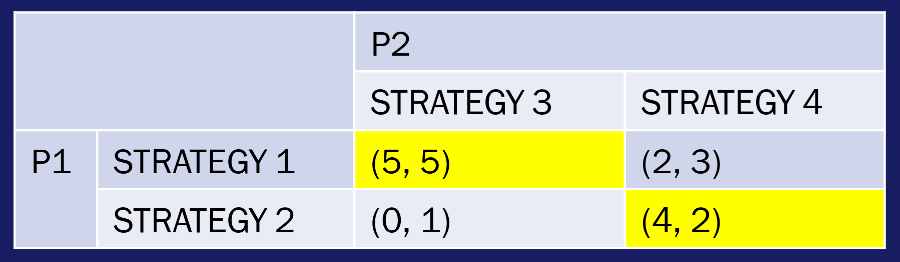
\includegraphics[width=.9\linewidth]{./images/nash-equilibrium-example.png}
\end{center}
\begin{itemize}
\item P1's strategy 2 is the \textbf{best response} to P2's strategy 4 (and vice versa).
\item P1's strategy 1 is the \textbf{best response} to P2's strategy 3 (and vice versa).
\end{itemize}

The cells coloured in \textbf{yellow} denote the \textbf{Nash equilibria}.
\subsection{Pareto optimality (Pareto efficiency)}
\label{sec:orgd756a02}
A state of affairs such that there is \textbf{no alternative state of affairs} that would \textbf{make some people better off without making at least one person worse off}.
\subsubsection{Example}
\label{sec:org39030b4}
\begin{center}
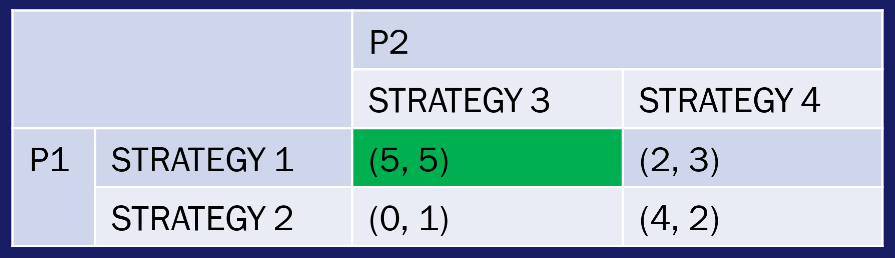
\includegraphics[width=.9\linewidth]{./images/pareto-optimal-example.png}
\end{center}

The cell coloured in \textbf{green} denotes a \textbf{Pareto-optimal} state of affairs.
\subsection{Validity of an argument}
\label{sec:org860a12c}
An argument is \textbf{valid} if, \textbf{assuming the truth of all its premises}, its conclusion must, by \textbf{logical necessity, be true too}.
\subsection{Soundness of an argument}
\label{sec:orgf2a43cc}
An argument is sound if \textbf{all of its premises are in fact true}, or it does not contain any \textbf{false premises}, and it is a \textbf{valid argument}.
\subsection{Classificatory moral commitments}
\label{sec:org5765b61}
Classificatory moral commitments are defined as the commitments that result from delineating the \textbf{scope of the moral domain}.
\subsection{Substantive moral commitments}
\label{sec:orgca71c4a}
Substantive moral commitments are defined as a \textbf{normative bias}.
\subsection{Normative neutrality}
\label{sec:org5c5da99}
\begin{itemize}
\item Normative neutrality between \textbf{competing moral standards} and \textbf{rules of conduct} is where the cut between \textbf{metaethics (2\textsuperscript{nd}-order theory)} and \textbf{normative theory (1\textsuperscript{st}-order theory)} is made.
\item Essentially, normative neutrality is what separates \textbf{metaethics and normative theory}.
\end{itemize}
\subsection{Axiology}
\label{sec:org2d456b4}
Axiology just means value theory.
\subsection{Reflective equilibrium}
\label{sec:org46ad23c}
Reflective equilibrium is a method of balancing moral principles and judgments to arrive at the content of justice.

 \newpage
\subsection{Eudaimonia}
\label{sec:orge10d557}
\begin{itemize}
\item Eudaimonia is a Greek word that means the state or condition of good spirit, and is often translated as happiness or welfare. In Aristotle's works, it means the highest human good.
\item It is a certain \textbf{flourishing} or the \textbf{sort of happiness worth seeking or having}.
\end{itemize}
\subsection{Hedonism}
\label{sec:orgc0a72da}

\subsubsection{Psychological hedonism}
\label{sec:orge3a0055}
Only \textbf{pleasure (happiness)} or \textbf{pain (unhappiness)} motivates us.
\subsubsection{Ethical hedonism}
\label{sec:org697e7a3}
Only \textbf{pleasure (happiness)} has \textbf{value} and only \textbf{pain (unhappiness)} has \textbf{disvalue}.
\subsection{Avant la lettre}
\label{sec:org682bb16}
Avant la lettre means that a concept exists even before a term is coined for it.
\subsection{Elenchus elenctic (The Socratic method)}
\label{sec:orgab6eeb5}
The Elenchus elenctic is a form of argumentative dialogue between individuals based on asking and answering questions.
\subsection{Agent}
\label{sec:org32dcf44}
The agent is the person who is performing an action.
\subsection{Patient}
\label{sec:org6e8e2d1}
The patient is the person on whom the action is performed.
\subsection{Prima facie}
\label{sec:org614f8df}
Prima facie is a Latin phrase meaning "at first sight", or "based on first impression". It is used in philosophy to indicate that something is sufficient or plausible unless rebutted.
\subsection{Virtue ethics}
\label{sec:org7f0fcef}
Virtue ethics is concerned with providing an account of the \textbf{moral virtues}.
\subsection{Virtual epistemology}
\label{sec:orga935093}
Virtue epistemology is concerned with providing an account of the \textbf{intellectual virtues}.

 \newpage
\section{Prior's paradox}
\label{sec:org5aeeadd}

\subsection{Assumptions}
\label{sec:org0d96c1c}
\begin{center}
\begin{tabular}{|m{5em}|m{25em}|}
\hline
Assumption & Description\\
\hline
\textbf{Dichotomy} assumption (A1) & All propositions may be categorised as either \textbf{ethical or non-ethical}\\
\hline
\textbf{Deductive argument} assumption (A2) & The \textbf{conclusion} of an argument cannot contain more information than its \textbf{premises}.\\
\hline
\end{tabular}
\end{center}
\subsection{Proposition}
\label{sec:orgfe5d51e}
Either tea drinking is common in England, or it ought to be the case that all New Zealanders are shot, formalised as \(p \vee Oq\). According to the dichotomy assumption, the proposition is either \textbf{ethical} or \textbf{non-ethical}.

\begin{center}
\begin{tabularx}{\textwidth}{|X|X|}
\hline
Horn 1 & Horn 2\\
\hline
\(p \vee Oq\) is ethical. & \(p \vee Oq\) is non-ethical.\\
\hline
If \(p \vee Oq\) is \textbf{ethical}, then: & If \(p \vee Oq\) is \textbf{non-ethical}, then:\\
P1 (non-ethical): Tea drinking is common in England. & P1 (non-ethical): Either tea drinking is common in England, or it ought to be the case that all New Zealanders are shot.\\
C (ethical): Therefore, either tea drinking is common in England, or it ought to be the case that all New Zealanders are shot. & P2 (non-ethical): Tea drinking is not common in England.\\
 & C (ethical): Hence, it ought to be the case that all New Zealanders are shot.\\
\hline
\end{tabularx}
\end{center}
 \newpage
\subsubsection{Dilemma}
\label{sec:orgee8ae23}
Whether we accept horn 1 or horn 2, we make \textbf{is-ought inferences} that are perfectly \textbf{valid}.
\begin{center}
\begin{tabularx}{\textwidth}{|X|X|X|X|X|}
\hline
Horn & Classification of \(p \vee Oq\) & Premise set & Conclusion set\\
\hline
Horn 1: \(p \vdash p \vee Oq\) & \(p \vee Oq\) is \textbf{ethical} & \textbf{Non-ethical} & \textbf{Ethical}\\
\hline
Horn 2: \(p \vee Oq, \neg p \vdash Oq\) & \(p \vee Oq\) is \textbf{non-ethical} & \textbf{Non-ethical} & \textbf{Ethical}\\
\hline
\end{tabularx}
\end{center}
Prior's paradox is a \textbf{dilemma without escape}. Since \textbf{Hume's Law}, even as a \textbf{one-way implication barrier}, is violated in every possible instance, it must be \textbf{false}. Hence, ethics is not \textbf{logically autonomous}.

 \newpage
\section{Defending Hume's Law}
\label{sec:orga268035}
\begin{enumerate}
\item Admit the \textbf{converse of the is-ought thesis}.
\item Exclude \textbf{contradictions} from the premise set \(\phi\). \(\phi\) should be defined as a \textbf{consistent or contradiction-free} set of \textbf{descriptive propositions}.
\item Exclude \textbf{tautologies} from the conclusion set \(\psi\). \(\psi\) should be defined as a \textbf{normative proposition} that is not already logically true.
\item Rule out \textbf{enthymematic arguments}. When the hidden premises of \textbf{enthymemes} are restored, the \textbf{premise set} \(\phi\) will have at least one \textbf{normative proposition}. Hence, these arguments will no longer be obvious counterexamples to Hume's Law.
\item Concede the \textbf{contraposition with "ought" implies the "can"} case. We should concede that \textbf{"cannot" implies "not obligatory"} yields a \textbf{special case} in which \(\phi \vdash \psi\).
\item Rule out \textbf{Geach-style conditionals} as non-ethical propositions. It gives rise to embedded "ought" propositions of the form \(Op \rightarrow Oq\).  \\

With \(Op \rightarrow Oq\), "ought" statements \(Op, Oq\) are being embedded into more complex logical structures, but there is no commitment to the truth or falsity of either \(Op\) or \(Oq\).
\item Rule out \textbf{mixed propositions} from the premise set \(\phi\) and the conclusion set \(\psi\). We can replace the \textbf{dichotomy} assumption with the \textbf{trichotomy} assumption, where all propositions may be categorised as either \textbf{ethical, non-ethical, or mixed}.
\end{enumerate}

 \newpage
\subsection{Issues with move 7}
\label{sec:org489c6c2}
Mixed propositions have an indispensable role in ethical reasoning and argumentation. Purely normative propositions are rarely encountered in the real world, outside the philosopher's laboratory.  \\

Examples include:
\begin{center}
\begin{tabular}{|m{25em}|m{5em}|}
\hline
Proposition in natural language & Formal representation\\
\hline
If you refrain from helping the old lady across the road, then you ought to be blamed. & \(\neg p \rightarrow Oq\)\\
\hline
Either you help the old lady across the road, or you ought to be blamed for not doing so. & \(p \vee Oq\)\\
\hline
It is necessarily the case that if p, then it is obligatory that q. & \(\Box (p \rightarrow Oq)\)\\
\hline
It is necessarily the case that for all \(x\), then \(Fx\), then it is obligatory that \(Gx\). & \(\Box \forall x (Fx \rightarrow Gx)\)\\
\hline
\end{tabular}
\end{center}
 \newpage
\subsection{Gerhard Schurz substitution}
\label{sec:orgd57312d}
\begin{itemize}
\item If a \textbf{mixed conclusion} \(\phi\) is derivable from a \textbf{purely non-ethical premise set} \(\phi\), then \(\psi\) is completely \textbf{O-irrelevant}.
\item Apply the \textbf{O-restricted propositional substitution function} \(\sigma\).
\item Substitute \(r\) (any proposition whatsoever) for \(q\) on exactly those occurrences of \(q\) outside the scope of \(O\), i.e.
\[p \text{ (non-ethical) } \vdash p \vee Oq,  \text{ (mixed) } \xrightarrow{\text{Apply } \sigma} p \text{ (non-ethical) } \vdash p \vee Or \text{ (mixed)}\]
\item The \textbf{O-restricted substitution} (\(\sigma\)) can be made without compromising the validity of the argument; hence, the mixed conclusion \(p \vee Oq\) is completely \textbf{O-irrelevant} relative to the premise set.
\item If a \textbf{mixed premise set} \(\phi\) is used to derive a \textbf{purely ethical conclusion} \(\psi\), then \(\phi\) is completely \textbf{is-irrelevant}.
\item Apply the \textbf{is-restricted propositional substitution function} \(\sigma'\).
\item Substitute \(r\) (any proposition whatsoever) for \(p\) on exactly those occurrences of \(p\) outside the scope of \(O\), i.e.
\[p \vee Oq, \neg p \text{ (mixed) } \vdash Oq \text{ (ethical) } \xrightarrow{\text{Apply } \sigma'} r \vee Oq, \neg r \text{ (mixed) } \vdash Oq \text{ (ethical)}\]
\item The \textbf{is-restricted substitution} (\(\sigma'\)) can be made without compromising the validity of the argument; hence, the \textbf{mixed premise set} \(p \vdash Oq, \neg p\) is completely \textbf{is-irrelevant} relative to the conclusion.
\end{itemize}

 \newpage
\subsection{Gibbard-Karmo-Singer semantics}
\label{sec:org3217756}
Gibbard-Karmo-Singer semantics is just a way of determining whether a set of propositions will result in ethical conclusions or not. It works like this:
\begin{enumerate}
\item Consider the truth value of the propositions in a possible world, such as the actual world we live in.
\item Consider the truth value of the propositions and conclusions in an ethical standard.
\item Swapping the ethical standard for another ethical standard without changing the world.
\item If the truth value of the conclusions changes when you change the ethical standard, like the conclusions change from true to false, then the conclusions are ethical.
\item Otherwise, the conclusions are non-ethical, because the ethical standard being used is not relevant to the truth value of the conclusions.
\item If the conclusions are non-ethical, and you want to figure out which possible worlds the set of propositions will result in ethical conclusions, swap out the world for another one and repeat steps 2 to 5.
\end{enumerate}
\subsection{Shorter's position}
\label{sec:orgb1136b8}
\begin{itemize}
\item The \textbf{conclusion} of an argument may be of \textbf{some importance (ethically speaking)} in deriving certain moral duties only if it is arrived at in some other way than employing an \textbf{is-ought inference}.
\item Hence, the \textbf{is-ought} inference is \textbf{not of importance (ethically speaking)}.
\item We need to distinguish between the \textbf{seriousness of the conclusion arrived at (ethically speaking)} and the \textbf{seriousness of the is-ought inference} by which the conclusion is arrived at.
\end{itemize}

 \newpage
\subsubsection{Tea drinking example}
\label{sec:orga185dea}
\begin{itemize}
\item P1 (non-ethical): Tea drinking is common in England.
\item C (ethical): Therefore, either tea drinking is common in England or it ought to be the case that all New Zealanders are shot.
\end{itemize}

\begin{center}
\begin{tabular}{|m{5em}|m{25em}|}
\hline
Step & Description\\
\hline
1 & P1 is either true or false.\\
\hline
2 & If P1 is true, then the \textbf{is-ought inference} lends support to C. However, C will be of no help or use to us in deriving certain moral duties.\\
 & \\
 & If P1 is false, then the \textbf{is-ought inference} lends no support to C. However, if P1 is false and C is true, then we can derive the duty to shoot all New Zealanders, and C may be of some importance (ethically speaking).\\
\hline
3 & Therefore, whether P1 is true or false, the \textbf{is-ought inference} is \textbf{useless}.\\
 & It either \textbf{renders C ethically useless insofar as it supports C (when P1 is true) or does not support C} (when P1 is false)\\
\hline
\end{tabular}
\end{center}
 \newpage
\subsubsection{Undertaker example}
\label{sec:org083957f}
\begin{itemize}
\item P1: Undertakers are church officers.
\item C: Therefore, undertakers ought to do whatever all church officers ought to do.
\item P2: All church officers ought to \(\phi\).
\end{itemize}

\begin{center}
\begin{tabular}{|m{5em}|m{25em}|}
\hline
Step & Description\\
\hline
1 & The \textbf{is-ought inference} either makes do without P2 or incorporates P2.\\
\hline
2 & If the \textbf{is-ought inference} makes do without P2, then it lends support to C. However, C will be \textbf{useless} without P2 as an undertaker can only derive a \textbf{concrete moral duty} with both P1 and P2.\\
 & \\
 & If the \textbf{is-ought inference} incorporates P2, then it lends support to \(C'\) (All undertakers ought to \(\phi\) rather than C (Undertakers ought to do whatever all church officers ought to do). Therefore, C will become \textbf{useless} with P2.\\
\hline
\end{tabular}
\end{center}

 \newpage
\section{Modal concepts}
\label{sec:org56d673a}
\begin{center}
\begin{tabularx}{1.2\textwidth}{|X|X|X|X|}
\hline
Mode & Domain & Categories & Logical state of play in 1951\\
\hline
Mode 1 (Alethic) & Truth & Necessary, Possible, and Contingent & \textbf{Alethic modal logic} with the \textbf{modal operators} \(\Box\) and \(\Diamond\)\\
\hline
Mode 2 (Epistemic) & Knowledge & Verified, Falsified, and Indeterminate & Minimal logical treatment\\
\hline
Mode 3 (Deontic) & Actions & Obligatory, Permissible, and Impermissible & Minimal logical treatment\\
\hline
Mode 4 (Existential) & Existence & Universal, Existential, and Empty & First-order predicate or quantificational logic (QL) with the quantifiers \(\forall\) and \(\exists\)\\
\hline
\end{tabularx}
\end{center}

 \newpage
\section{Deontic logic}
\label{sec:orgfe49aef}
Deontic logic is a field of philosophical logic that is concerned with obligation, permission, and related concepts. The word "deontic" comes from the Greek word "deon" which means "that which is binding or proper".
\subsection{Analogies between the deontic mode and the alethic mode}
\label{sec:orgae5d1b7}

\subsubsection{Analogy 1}
\label{sec:org747880a}
There are 2 operators.
\begin{itemize}
\item Alethic mode
\[\Box p \defequal \neg \Diamond \neg p\]
\[\Diamond \defequal \neg \Diamond \neg p\]

\(\Box\) and \(\Diamond\) are De Morgan duals.

\item Deontic mode
\[Op \defequal \neg P \neg p\]
\[Pp \defequal \neg O \neg p\]

\(O\) and \(P\) are De Morgan duals.
\end{itemize}
\subsubsection{Analogy 2}
\label{sec:org962101b}
There are \textbf{5 statuses} that can be defined in terms of \textbf{2 operators}.
\begin{center}
\begin{tabularx}{\textwidth}{X|X}
Source (alethic mode) & Target (deontic mode)\\
\hline
It is \textbf{necessary} that \(p \ (\Box p)\) & It is obligatory that \(p \ (Op)\)\\
It is \textbf{possible} that \(p \ (\Diamond p)\) & It is \textbf{permissible} that \(p \ (Pp)\)\\
It is \textbf{impossible} that \(p \ (\neg \Diamond p)\) & It is \textbf{impermissible} that \(p (\neg Pp)\)\\
It is \textbf{non-necessary} that \(p \ (\neg \Box p)\) & It is \textbf{omissible} that \(p (\neg Op)\)\\
It is \textbf{contingent} that \(p \ (\Diamond p \wedge \neg \Box p)\) & It is \textbf{optional} that \(p (Pp \wedge \neg Op)\)\\
\end{tabularx}
\end{center}
\subsubsection{Analogy 3}
\label{sec:orgf22ed37}
There are \textbf{5 statuses} that can be represented by a \textbf{threefold partition}.
\begin{center}
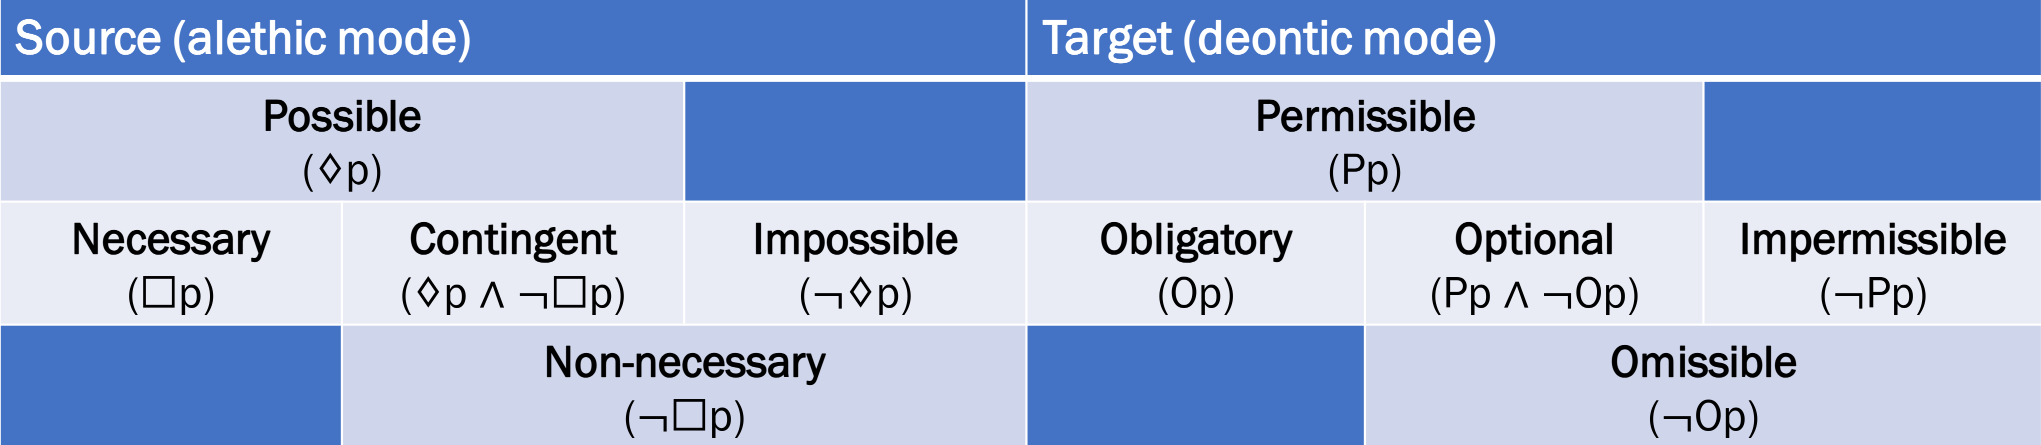
\includegraphics[width=.9\linewidth]{./images/threefold-partition-analogy.png}
\end{center}
\subsubsection{Analogy 4}
\label{sec:org9b9ed6a}
There is \textbf{1 square of opposition}.
\begin{center}
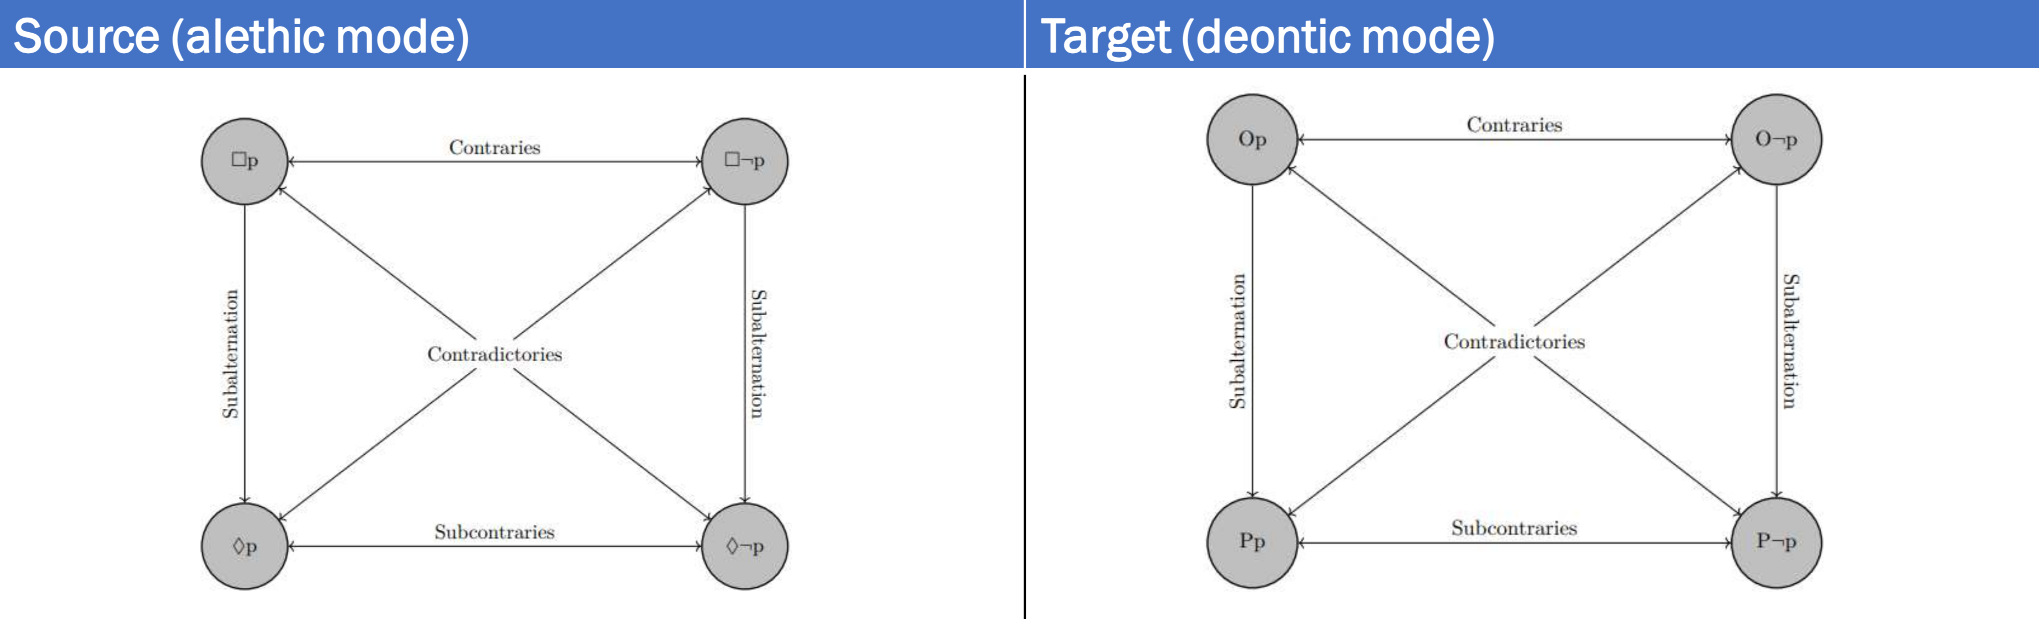
\includegraphics[width=.9\linewidth]{./images/one-square-of-opposition-analogy.png}
\end{center}

\begin{itemize}
\item Two propositions are \textbf{contradictories} if and only if the \textbf{truth} of one implies the \textbf{falsity} of the other.
\item Two propositions are \textbf{contraries} if and only if they cannot both be \textbf{true} but can both be \textbf{false}.
\item Two propositions are \textbf{subcontraries if and only if they cannot both be false} but can both be \textbf{true}.
\item Two propositions are in a \textbf{subalternation} relation if and only if the \textbf{truth} of the first proposition \textbf{(superaltern)} implies the \textbf{truth} of the second \textbf{(subaltern)} but NOT vice versa.
\end{itemize}
\subsubsection{In summary}
\label{sec:org9f806c2}
\begin{center}
\begin{tabular}{|m{5em}|m{25em}|}
\hline
Analogy & Description\\
\hline
Analogy 1 & There are \textbf{2 operators}.\\
 & Source (alethic mode): \(\Box, \Diamond\)\\
 & Target (deontic mode): \(O, P\)\\
\hline
Analogy 2 & There are \textbf{5 statuses}.\\
 & Source (alethic mode): \textbf{necessity, possibility, impossibility, non-necessity, contingency}\\
 & Target (deontic mode): \textbf{obligatoriness, permissibility, impermissibility, omissibility, optionality}\\
\hline
Analogy 3 & These \textbf{5 statuses} can be represented by a \textbf{threefold partition}.\\
 & Source (alethic mode): \textbf{necessity, contingency, impossibility}\\
 & Target (deontic mode): \textbf{obligatoriness, optionality, impermissibility}\\
\hline
Analogy 4 & There is \textbf{1 square of opposition}.\\
 & Source: (alethic mode): \textbf{modal square of opposition}\\
 & Target: (deontic mode): \textbf{deontic square of opposition}\\
\hline
\end{tabular}
\end{center}
\subsection{Disanalogies}
\label{sec:org09fb1cf}
\begin{center}
\begin{tabularx}{\textwidth}{|X|X|X|}
\hline
Disanalogy & Source (alethic mode) & Target (deontic mode)\\
\hline
Disanalogy 1 & \(\Box p \rightarrow p\) & \(\neg (Op \rightarrow p)\)\\
 & If \(p\) is \textbf{true} across ALL possible worlds that are \textbf{accessible}, the \(p\) must be \textbf{true} in the \textbf{actual world} \(@\). & It does not follow from the fact that the action described by \(p\) is \textbf{obligatory} that the action is performed in the \textbf{actual world} \(@\).\\
\hline
Disanalogy 2 & \(p \rightarrow \Diamond p\) & \(\neg (p \rightarrow Pp)\)\\
 & If \(p\) is \textbf{true} in the \textbf{actual world} \(@\), then \(p\) must be \textbf{true} in at least one possible world that is \textbf{accessible}. & It does NOT follow from the fact that the action is performed in the \textbf{actual world} \(@\) that is \textbf{permissible}.\\
\hline
\end{tabularx}
\end{center}
\subsection{Components}
\label{sec:orgfa32901}
\begin{center}
\begin{tabularx}{\textwidth}{|X|X|X|}
\hline
Component of the logical system & Elaboration\\
\hline
\textbf{Alphabet} & The \textbf{alphabet} of \textbf{deontic logic} is an extension of the \textbf{alphabet} of \textbf{propositional logic} to include the \textbf{deontic operators} \(O\) and \(P\).\\
\hline
\textbf{Syntax} & The \textbf{syntax} of \textbf{deontic logic} is an extension of the \textbf{syntax} of \textbf{propositional logic} to handle \textbf{well-formed formulae (wffs)} containing at least one \textbf{deontic operator}.\\
\hline
\textbf{Semantics} & The \textbf{semantics} of \textbf{deontic logic} is of the form \(\langle W, S, @ \rangle\), where \(W\) denotes a \textbf{set of worlds}, \(S\) denotes a \textbf{binary relation of moral satisfaction} between worlds, and \(@\) denotes the \textbf{actual world (privileged)}.\\
\hline
\textbf{Proof theory} & The \textbf{proof theory} of \textbf{deontic logic} comprises a set of \textbf{definitions, axioms}, and \textbf{rules of inference}.\\
 & This \textbf{proof theory}, with its reliance on \textbf{axioms}, is known as \textbf{Hilbert-style proof theory}.\\
\hline
\end{tabularx}
\end{center}
\subsection{Proof theory}
\label{sec:org9bfa5b5}
\begin{center}
\begin{tabularx}{\textwidth}{|X|X|X|}
\hline
Definitions & Axioms & Rules of inference\\
\hline
Definition 1: & (T) All \textbf{tautologous well-formed formulae} from \textbf{propositional logic}. & (\(\rightarrow_{E1}\) or \emph{modus ponens}) \(p \rightarrow q\), \(p \vdash q\)\\
 &  & \\
\(Op \defequal \neg P \neg p\) & (NC) \(\neg (Op \wedge O \neg p)\) & \\
 &  & \\
 & It cannot be the case that both \(p\) and \(\neg p\) are \textbf{obligatory}. & \\
\hline
Definition 2: & (K) \(O(p \rightarrow q) \rightarrow (Op \rightarrow Oq)\) & \\
 &  & \\
 & If performing the action described in p \textbf{commits} me to performing the action described in \(q\), if \(p\) is \textbf{obligatory}, \(q\) will be \textbf{obligatory} too. & \\
 &  & \\
\(Pp \defequal \neg O \neg P\) & (NEC) \(\vdash p \rightarrow \vdash Op\) & \\
 &  & \\
 & If \(p\) is \textbf{tautological}, then \(Op\) is also \textbf{tautological}. & \\
\hline
\end{tabularx}
\end{center}

 \newpage
\subsection{Monotonicity of entailment (RM)}
\label{sec:org6c5b9bc}
The monotonicity of entailment just means that if a sentence follows deductively from a given set of sentences, then it also follows deductively from any superset of those sentences. It is formalised as such:
\[\text{(RM): } (\vdash p \rightarrow p) \rightarrow (\vdash Op \rightarrow Oq)\]
\subsubsection{Proof}
\label{sec:org218a627}
\begin{enumerate}
\item Assume that \(\vdash p \rightarrow q\)
\item \(\therefore (\vdash p \rightarrow q) \rightarrow \vdash O(p \rightarrow q)\)
\item \(\therefore \ \vdash O(p \rightarrow q)\)
\item \(\therefore \ \vdash O(p \rightarrow q) \rightarrow \vdash Op \rightarrow Oq\)
\item \(\therefore \ \vdash Op \rightarrow Oq\)
\item \(\therefore (\vdash p \rightarrow q) \rightarrow (\vdash Op \rightarrow Oq)\)
\end{enumerate}
\subsection{Corollary of the monotonicity of entailment (Corollary of RM)}
\label{sec:orgc9efc37}
The corollary of the monotonicity of entailment is that if a given argument is deductively valid, it cannot become invalid by the addition of extra premises. It is formalised as such:
\[\text{(Corollary of RM): } \vdash Op \rightarrow O(p \vee q)\]
\subsubsection{Proof}
\label{sec:org3afcc0d}
\begin{enumerate}
\item \(\vdash p \rightarrow (p \vee q)\)
\item \(\therefore (\vdash p \rightarrow (p \vee q)) \rightarrow (\vdash Op \rightarrow O(p \vee q))\)
\item \(\therefore \ \vdash Op \rightarrow O(p \vee q)\)
\end{enumerate}
\subsection{Theorem T1}
\label{sec:orgc6fb14f}
\[(T1) \vdash O(p \wedge q) \rightarrow Oq\]
\subsubsection{Proof}
\label{sec:orge53d3f7}
\begin{enumerate}
\item \(\vdash (p \wedge q) \rightarrow q\)
\item \(\therefore (\vdash (p \wedge q) \rightarrow q) \rightarrow (\vdash O(p \wedge q) \rightarrow Oq)\)
\item \(\therefore \ \vdash O(p \wedge q) \rightarrow Oq\)
\end{enumerate}
\subsection{Paradoxes of obligation}
\label{sec:orgd9c16b4}

\subsubsection{Paradox of the gentle murderer}
\label{sec:org5c7048e}
Propositions (P):
\begin{enumerate}
\item It ought to be the case that A does not kill his mother.
\item If A does kill his mother, then it ought to be the case that A kills her gently.
\item A does kill his mother.
\end{enumerate}

Proof:
\begin{enumerate}
\item \(O \neg p\), where \(p\) denotes "A kills his mother" (from P1).
\item \(p \rightarrow Oq\), where \(q\) denotes "A kills his mother gently" (from P2).
\item \(p\) (from P3).
\item \(\therefore Oq\) (from 2, 3, and \(\rightarrow_{E1}\) or \emph{modus ponens}).
\item \(\therefore \ \vdash q \rightarrow p\) (from T).
\item \(\therefore (\vdash q \rightarrow p) \rightarrow (\vdash Oq \rightarrow Op)\) (from RM, uniformly substitute \(p\) for \(q\) and vice versa).
\item \(\therefore \ \vdash Oq \rightarrow Op\) (from 5, 6, and \(\rightarrow_{E1}\) or \emph{modus ponens}).
\item \(\therefore Op\) (from 4, 6, and \(\rightarrow_{E1}\) or \emph{modus ponens}).
\end{enumerate}

Using the monotonicity of entailment, it follows that A should kill his mother, which is an odd thing to say.
\subsubsection{Ross' paradox}
\label{sec:org329ee6b}
Propositions (P):
\begin{enumerate}
\item It is obligatory that the letter is mailed.
\item Therefore, it is obligatory that the letter is mailed, or the letter is burnt.
\end{enumerate}

Proof:
\begin{enumerate}
\item \(Op\), where \(p\) denotes "the letter is mailed"
\item \(\vdash Op \rightarrow O(p \vee q)\) (Corollary of RM)
\item \(\therefore O(p \vee q)\), where \(q\) denotes "the letter is burnt" (from 1, 2, and \(\rightarrow_{E1}\) or \emph{modus ponens})
\end{enumerate}

It is odd to say that P1 and the corollary of RM entail an obligation that can be fulfilled by burning the letter (presumably an \textbf{impermissible} action).
\subsubsection{The Good Samaritan paradox}
\label{sec:org8aad76e}
Propositions (P):
\begin{enumerate}
\item It ought to be the case that A helps B, who has been robbed.
\item Therefore, it ought to be the case that B has been robbed.
\end{enumerate}

Proof:
\begin{enumerate}
\item \(O(p \wedge q\), where \(p\) denotes "A helps B" and \(q\) denotes "B has been robbed" (from P1).
\item \(\vdash O(p \wedge q) \rightarrow Oq\) (T1)
\item \(\therefore Oq\) (from 1, 2, and \(\rightarrow_{E1}\) or \emph{modus ponens})
\end{enumerate}

It is odd to say that from P1 and T1, it follows that B's being robbed is also obligatory.
\subsection{Resolving the paradoxes}
\label{sec:org402bc7e}
\begin{center}
\begin{tabularx}{1.2\textwidth}{|X|X|X|X|}
\hline
Response & Paradox of the gentle murderer & Ross' paradox & The good Samaritan paradox\\
\hline
Response 1: Distinguish between \textbf{non-derivatively obligatory} and \textbf{derivatively obligatory} actions. & Refrain from killing your mother (\textbf{non-derivatively obligatory}) & Mail the letter (\textbf{non-derivatively obligatory}) & Help someone who is in need (\textbf{non-derivatively obligatory})\\
 & Kill your mother (derived from RM and \textbf{impermissible}) & Burn the letter (derived from the \textbf{corollary} of RM and \textbf{impermissible}) & Rob the individual who has been robbed (derived from T1 and \textbf{impermissible})\\
\hline
Response 2: Reject RM & RM gives rise to the \textbf{gentle murderer paradox}. & The \textbf{corollary of RM} gives rise to \textbf{Ross' paradox}. & T1, a theorem derived from RM, gives rise to the \textbf{good Samaritan paradox}.\\
\hline
Response 3: Introduce a \textbf{dyadic (2-placed) version of deontic logic}. & O(\(\neg\) murder \(\vert\) T) (\textbf{unconditional obligation}) & \(O(\)mail \(\vert\) text has been written\()\) (\textbf{conditional obligation}) & \(O(\)help B \(\vert\) B has been robbed\()\) (\textbf{conditional obligation})\\
 & O (gentle murder \(\vert\) murder) (\textbf{conditional obligation} if the \textbf{unconditional obligation} is violated) &  & \\
 &  &  & \\
 & We cannot derive an \textbf{unconditional obligation} to murder. & We cannot derive an \textbf{obligation} to mail or burn the letter. & We cannot derive an \textbf{obligation} for B to have been robbed.\\
 & \(\nvdash\) \(O(\)murder \(\vert\) T\()\) & \(\nvdash\) \(O(\)mail \(\vee\) burn\()\) & \(\nvdash\) \(O(\)B has been robbed\()\)\\
\hline
\end{tabularx}
\end{center}
\subsection{Mimamsa deontic logic}
\label{sec:org1b84cfd}
\begin{itemize}
\item Classical deontic logic is a \textbf{monadic (1-placed)} system:
\[O(\_)\]
\item At least some systems of \textbf{deontic logic} are \textbf{dyadic (2-placed)} systems:
\[O(\_ | \_)\]
\end{itemize}

It ought to be the case that A helps B and B has been robbed. Denoting \(p\) as "A helps B" and \(q\) as "B has been robbed":
\begin{itemize}
\item Formal representation under \textbf{monadic deontic logic}:
\[O(p \wedge q)\]
\item Formal representation under \textbf{dyadic deontic logic}:
\[O(p | q)\]
\end{itemize}
\subsubsection{Dyadic deontic operator \(O(\phi | \theta)\)}
\label{sec:orga0c1177}
The \textbf{dyadic deontic operator} \(O(\phi | \theta)\) is used in \textbf{dyadic deontic logic} to represent \textbf{conditional obligations}. \(\phi\) represents the \textbf{main argument} and \(\theta\) represents the \textbf{triggering condition}.

\begin{itemize}
\item It is necessarily the case that given \(p\), it is obligatory that \(q\).
\[\Box O (q | p)\]
\item There is a \textbf{conditional obligation} that \(q\), given \(p\).
\[\Box O (q | p)\]
\item There is an \textbf{unconditional obligation} that \(q\), given that anything is the case.
\[O (q | T)\]
\end{itemize}
\section{Inductive reasoning}
\label{sec:org38c9449}
\[\phi \vdash^{I}_{P} \psi\]

Where:
\begin{itemize}
\item \(\phi\) is the set of premises, which potentially includes the knowledge base
\item \(\vdash\) represents that \(\psi\) is provable from \(\phi\)
\item \(I\) refers to the inductive mode
\item \(P\) refers to the inferential mechanism of the calculus of probability
\item \(\psi\) is the set of conclusions derived from the set of premises
\end{itemize}
\subsection{Newcomb's paradox (Newcomb's problem)}
\label{sec:orga63f5d5}
There is a reliable predictor, another player, and two boxes designated A and B. The player is given a choice between taking only box B or taking both boxes A and B. The player knows the following:
\begin{itemize}
\item Box A is transparent and always contains a visible \$1000.
\item Box B is opaque, and its content has already been set by the predictor:
\begin{itemize}
\item If the predictor has predicted that the player will take boxes A and B, then box B contains nothing.
\item If the predictor has predicted that the player will take only box B, then box B contains \$1,000,000.
\end{itemize}
\end{itemize}

The player does not know what the predictor predicted, or what box B contains while making the choice.
\subsection{Philosophical principles}
\label{sec:org687dccc}
\begin{center}
\begin{tabularx}{\textwidth}{|X|X|}
\hline
Principle & Description\\
\hline
The \textbf{principle of multiple explanations}. (Epicurus, c. 300 B.C.E.) & If multiple theories \(H_1, H_2\), and so on, are \textbf{consistent} with our observation \(E\), then we should retain ALL these theories \(H_1, H_2\), and son on.\\
\hline
The \textbf{uniformity of nature principle}. (Hume, 1739/40) & Nature is \textbf{sufficiently uniform} that \textbf{unobserved instances} in the \textbf{future} will resemble \textbf{observed instances} in the \textbf{future} will resemble \textbf{observed instances} in the \textbf{past}.\\
\hline
\textbf{Occam's razor principle}. (William of Ockham, 14th century C.E.) & Entities should NOT be multiplied beyond necessity.\\
\hline
\end{tabularx}
\end{center}
 \newpage
\subsection{Bayes' theorem}
\label{sec:org0b14831}
\[(BT) P(H | E) = \frac{P(E | H) \times P(H)}{P(E)}\]

Where:
\begin{itemize}
\item \(BT\) refers to the finite set of rules of inferences, which is \textbf{Bayes' rule} or \textbf{Bayes' theorem}.
\item \(P\) is the probability of something
\item \(H\) is the hypothesis
\item \(E\) is the evidence
\item \(P(H | E)\) means the likelihood of \(H\) given \(E\), it also refers to the \textbf{posterior probability}
\item \(P(E | H)\) means the likelihood of \(E\) given \(H\)
\item \(P(H)\) refers to the \textbf{prior probability} of hypothesis \(H\) without ANY given conditions
\end{itemize}
\subsection{Conditional probability}
\label{sec:orgcbae45a}
\[P(A | B) = \frac{P (A \cap B)}{P(B)}, \text{ if } P(B) \ne 0\]

Where:
\begin{itemize}
\item \(P\) is the probability of something
\item \(A\) is an event
\item \(B\) is another event
\item \(\cap\) is the intersection of event \(A\) and \(B\), i.e. the probability of event \(A\) and event \(B\) happening
\end{itemize}
\subsection{Deductive vs inductive reasoning}
\label{sec:org2bc8381}
\begin{center}
\begin{tabularx}{\textwidth}{|X|X|}
\hline
Deductive reasoning & Inductive reasoning\\
\hline
We reason under \textbf{certainty} concerning propositions that are either \textbf{true} or \textbf{false}. & We reason under \textbf{uncertainty} concerning propositions in which we have \textbf{differing degrees of belief}.\\
\hline
\textbf{Deductive reasoning} is \textbf{monotonic}. & \textbf{Inductive reasoning} is \textbf{non-monotonic}.\\
If \(\phi \vdash \psi\), then adding more information \(\lambda\) to the \textbf{premise set} \(\phi\) will NOT invalidate out \textbf{conclusion} that \(\psi\). & Although it may be \textbf{true} that \(\phi \vdash \psi\), it need NOT be the case that \((\phi \wedge \lambda) \vdash \psi\). \(\lambda\) may constitute \textbf{new evidence}, forcing us to \textbf{retract or revise} our \textbf{conclusion} that \(\psi\).\\
\hline
\textbf{Deductive reasoning} is \textbf{non-ampliative}. & \textbf{Inductive reasoning} is \textbf{ampliative}.\\
\textbf{Deductive reasoning} unpacks the information content of the \textbf{premise set} \(\phi\), such that the information contained in the \textbf{conclusion set} \(\psi\) is already present (albeit in implicit form) in \(\phi\). & The information in the \textbf{conclusion} that \(\psi\) \textbf{exceeds and amplifies} the information content of the \textbf{premise set} \(\phi\).\\
\hline
\end{tabularx}
\end{center}
 \newpage
\subsection{Axioms of probability (Kolmogorov theorem)}
\label{sec:org3a4421f}

\subsubsection{Degrees of belief}
\label{sec:org4ffeb70}
The \textbf{degrees of belief} are constrained by a finite set of \textbf{axioms of probability}. Any probability function \(P\) must satisfy the following axioms:

\begin{center}
\begin{tabularx}{\textwidth}{|X|X|}
\hline
Axiom & Description\\
\hline
K1 (\textbf{non-negativity}) & \(P(A) \ge 0\) in \textbf{sample space} \(\Omega\), where \(P(A)\) is the \textbf{probability} of \textbf{outcome} \(A\).\\
\hline
K2 (\textbf{normalisation}) & \(P(\Omega) = 1\)\\
\hline
K3 (\textbf{addition rule}) & \(P (A \cup B) = P(A) + P(B) - P(A \cap B)\)\\
 & If \(A\) and \(B\) are \textbf{mutually exclusive}, then \((A \cap B) = \emptyset\) and \(P(A \cap B) = 0\).\\
 & \(\therefore P(A \cup B) = P(A) + P(B)\)\\
\hline
K4 (\textbf{complement rule}) & \(P(\bar{A}) = P(\Omega) - P(A) = 1 - P(A)\)\\
\hline
\end{tabularx}
\end{center}
\subsubsection{Ruled-out scenarios}
\label{sec:org5bf9c07}
A set of \textbf{outcomes} is \textbf{jointly exhaustive} if these \textbf{outcomes} encompass the entire \textbf{sample space} \(\Omega\). In other words, at least one of these \textbf{outcomes} must occur.  \\

The \textbf{axioms of probability} rule out the following scenarios:
\begin{center}
\begin{tabularx}{\textwidth}{|X|X|}
\hline
Scenario & Axiom ruling out the scenario\\
\hline
The assignment of \textbf{negative probability values} to individual \textbf{outcomes} & K1 or \textbf{non-negativity}\\
\hline
The assignment of \textbf{probability values} to \textbf{jointly exhaustive and mutually exclusive outcomes} that sum to \(> 1\). & K2 or \textbf{normalisation}\\
\hline
The assignment of \textbf{probability values} to \textbf{jointly exhaustive outcomes} that sum to \(< 1\). & K2 or \textbf{normalisation}\\
\hline
The assignment of a \textbf{probability value} other than \(1 - p\) to \(\bar{A}\), when an agent assigns a \textbf{probability value} \(p\) to some \textbf{outcome} \(A\). & K4 or \textbf{complement rule}\\
\hline
\end{tabularx}
\end{center}
\subsection{Axioms of expected utility theory (von-Neumann-Morgenstern theorem)}
\label{sec:org0754fac}

\subsubsection{Degrees of preference}
\label{sec:org4384751}
The \textbf{degrees of preference} are constrained by the \textbf{axioms of expected utility theory}.

Any agent faced with a system \(U\) of alternative entities \(u, v, \ldots\) must satisfy the following axioms:
\begin{center}
\begin{tabular}{|m{7em}|m{25em}|}
\hline
Scenario & Axiom ruling out the scenario\\
\hline
VM1 (\textbf{completeness}) & For every \(u\) and \(v\), one and only one of the following relations holds:\\
 & \(u \succ v\) (the agent \textbf{prefers} \(u\) to \(v\))\\
 & \(v \succ u\) (the agent \textbf{prefers} \(v\) to \(u\))\\
 & \(u \sim v\) (the agent is \textbf{indifferent} between \(u\) and \(v\))\\
 & \\
 & Alternatively, for every \(u\) and \(v\), either \(u \succeq v\) or \(v \succeq u\).\\
\hline
VM2 (\textbf{transitivity}) & For every \(u, v\) and \(w, u \succ v\) and \(v \succ w\) imply that \(u \succ w\).\\
 & \\
 & Alternatively, for every \(u, v,\) and \(w\), if \(u \succeq v\) and \(v \succeq w\), then \(u \succeq w\).\\
\hline
VM3 (\textbf{independence of irrelevant alternatives}) & For every \(u, v,\) and \(w\), suppose that \(u \succeq v\) and a \textbf{third irrelevant alternative} \(w\) is present.\\
 & The \textbf{order of preference} of \(u\) over \(v (u \succeq v)\) holds, independently of the presence of absence of the \textbf{third irrelevant alternative} \(w\).\\
\hline
VM4 (\textbf{continuity}) & Let \(L\) denote a \textbf{lottery} whose 2 possible \textbf{outcomes} are \(u\) and \(v\), \(L \defequal \{u, v\}\)\\
 & \(P(u) = \alpha\) and \(P(v) = 1 - \alpha)\), where \(0 < \alpha < 1\)\\
 & \\
 & For every \(u, v,\) and \(w, v \succ w \succ u\) implies the following:\\
 & The existence of an \(\alpha\) such that \(w \succ L\) when \(1 - \alpha\) or \(P(v)\) is \textbf{sufficiently small}.\\
 & The existence of an \(\alpha\) such that \(w \sim L\) at a certain value of \((1 - \alpha)\).\\
 & The existence of an \(\alpha\) such that \(L \succ w\) when \(1 - \alpha\) or \(P(v)\) is \textbf{sufficiently large}.\\
\hline
\end{tabular}
\end{center}
\subsubsection{Ruled-out scenarios}
\label{sec:org01fb52b}
The \textbf{axioms of expected utility theory} rule out the following scenarios:
\begin{center}
\begin{tabularx}{\textwidth}{|X|X|}
\hline
Scenario & Axiom ruling out the scenario\\
\hline
The agent prefers neither alternative to another nor remains \textbf{indifferent} between both alternatives. & VM1 (\textbf{completeness})\\
\hline
The agent preferring \(u\) to \(v\) and \(v\) to \(w\) but remaining \textbf{indifferent} between \(u\) and \(w\). & VM (\textbf{transitivity})\\
\hline
The \textbf{decoy effect}. & VM3 (\textbf{independence of irrelevant alternatives})\\
\hline
The impossibility of an agent preferring lottery \(L\) to \(w\), where \(v \succ w \succ u\) and \(L \defequal \{u, v\}\) & VM4 (\textbf{continuity})\\
\hline
\end{tabularx}
\end{center}

\begin{itemize}
\item According to the \textbf{Cox-Jaynes model}, any system \textbf{reasoning under uncertainty} and in terms of \textbf{degrees of belief} will conform to the \textbf{axioms of probability}.
\item Furthermore, if the \textbf{axioms of expected utility theory} are satisfied, then the agent is said to be \textbf{rational} and the \textbf{preferences} can be represented by a \textbf{utility function}.
\end{itemize}

 \newpage
\subsection{Bayesian decision theory}
\label{sec:org5d4bab5}
\begin{itemize}
\item \textbf{Standard decision theory} addresses \textbf{individual decision-making} under \textbf{uncertainty}.
\item \textbf{Standard decision theory} incorporates the \textbf{axioms of probability} (K1 - K4) and the \textbf{axioms of expected utility theory} (VM1 - VM4).
\end{itemize}

\textbf{Bayesian decision theory} incorporates \textbf{standard decision theory} and \textbf{Bayesian epistemology} (BT):
\begin{center}
\begin{tabular}{|m{2em}|m{28em}|}
\hline
Step & Description\\
\hline
1 & Identify \(n\) alternative courses of action \(\phi_1, \phi_2, \ldots, \phi_n\) and their \(m\) associated possible outcomes, where \(\{M, n\} \in \mathbb{N}\).\\
\hline
2 & Characterise each action \(\phi_i\) in terms of its possible outcomes \(s_j\), where \(\{i, j\} \in \mathbb{N}, i \in (0, n]\) and \(j \in (0, m]\).\\
\hline
3 & Assign \textbf{prior probabilities} to each outcome \(P(s_j \vert \phi_i)\) in accordance with K1 - K4.\\
\hline
4 & Assign \textbf{utility values} to each outcome \(U(s_j \cap \phi_i)\) in accordance with VM1 - VM4.\\
\hline
5 & Gather evidence and \textbf{update probabilities} by applying Bayesian epistemology.\\
\hline
6 & Multiplying the \textbf{updated probability} and the \textbf{utility values} each \textbf{outcome} \(s_j\) relative to \(\phi_i\).\\
\hline
7 & Sum the products across each section \(\phi_i\) to determine its \textbf{expected utility}.\\
\hline
8 & Select the action \(\phi_i\) with the \textbf{highest expected utility} as the \textbf{morally right action}.\\
\hline
\end{tabular}
\end{center}
\subsection{Jeffrey-Bolker theory}
\label{sec:org123cc71}
Jeffrey-Bolker's expected utility theory is an example of \textbf{evidential decision theory}. It relies on a boolean algebra \(\Omega\) that consists of:

\begin{center}
\begin{tabular}{l|l}
Formal representation & Description\\
\hline
\(A, B, C\), etc. & \textbf{Propositions} as elements of \(\Omega\).\\
\(\bar{A}\) & \textbf{Negation}, such that if \(A \in \Omega\), then \(\bar{A} \in \Omega\).\\
\(A \cup B\) & \textbf{Disjunction}, such that if \(A, B \in \Omega\), then \(A \cup B \in \Omega\).\\
\(\top\) & \textbf{Tautology}.\\
\(\bot\) & \textbf{Contradiction} or negation of \(\top\).\\
\(\succeq\) & A coherent \textbf{preference order relation} over \(\Omega'\).\\
\end{tabular}
\end{center}
\subsubsection{Strategy}
\label{sec:org184f44c}
Jeffrey aims to recommend a \textbf{Bayesian model of deliberation} and a corresponding \textbf{theory of preference}.

\begin{center}
\begin{tabular}{|m{2em}|m{28em}|}
\hline
Move & Description\\
\hline
1 & Identify the \textbf{Bayesian principle of deliberation}. According to this principle, we rank actions \(\phi_1, \phi_2, \ldots, \phi_n\) in order of \textbf{preference}.\\
 & \\
 & Given a \textbf{coherent preference ranking}, we can discover a pair of \textbf{probability and desirability assignments} (roughly corresponding to the \textbf{probability} and \textbf{utility value assignments}) to propositions describing the performance of these actions.\\
\hline
2 & Introduce the \textbf{coherence} assumption. According to this assumption, the agent's \textbf{preference ranking} has the following properties:\\
 & \\
 & Property 1: \textbf{Coherence}\\
 & There is an underlying set of \textbf{probabilities and desirabilities} that yield the \textbf{preference ranking} via the \textbf{Bayesian principle of deliberation}.\\
 & \\
 & Property 2: \textbf{Defeasibility}\\
 & \textbf{Experience and reflection} constantly force the agent to \textbf{revise their agent preference ranking}.\\
\hline
3 & Characterise the \textbf{desirability function (des)} and the \textbf{probability measure (prob)}. The \textbf{desirabilities (des)} of the \textbf{basic cases} may be any set of numbers, independent of the \textbf{probabilities} \(\text{des} A > 0\) if \(A\) is \textbf{good}, \(\text{des } A = 0\) if \(A\) is \textbf{indifferent}, \(\text{des } A < 0\) if \(A\) is \textbf{bad}.\\
 & \\
 & The \textbf{probabilities (prob)} of the \textbf{basic cases} may be any set of non-negative numbers that sum to 1 (\(P(A) \ge 0, P(\Omega) = 1\)).\\
\hline
\end{tabular}
\end{center}
\subsubsection{Example}
\label{sec:org6133cf2}
\begin{center}
\begin{tabular}{l|l|l}
Event & \(L\) (live to age 65 or more) & \(\bar{L}\) (die before age 65)\\
\hline
\(S\) (smoke) & Best (\(S \cap L\)) & 3\textsuperscript{rd} best (\(S \cap \bar{L}\))\\
\hline
\(\bar{S}\) (quit) & 2\textsuperscript{nd} best (\(\bar{S} \cap L\)) & Worst (\(\bar{S} \cap \bar{L}\))\\
\end{tabular}
\end{center}
\subsubsection{Non-Bayesian deliberation of the example}
\label{sec:org3d10934}
According to the \textbf{syllogistic line of reasoning}:
\begin{itemize}
\item P1: Either \(L\) or \(\bar{L}\).
\item P2: If \(L\), then \(S\) is more desirable than \(\bar{S}\).
\item P3: If \(\bar{L}\), then (equally) \(S\) is more desirable than \(\bar{S}\).
\item C: \(\therefore S\) is more desirable than \(\bar{S}\) (\textbf{fallacious})
\end{itemize}

This \textbf{fallacious line of reasoning} wrongly assumes that the \textbf{4 possible action-outcome pairs} are \textbf{equiprobable}:
\[P(S \cap L) = P(S \cap \bar{L}) = P(\bar{S} \cap L) = P (\bar{S} \cap \bar{L}) = 0.25\]
\begin{align*}
U(S) &= \frac{P(S \cap L) \times v(S \cap L) + P(S \cap \bar{L}) \times v(S \cap \bar{L})}{P(S \cap L + P(S \cap \bar{L}))} \\
&= \frac{P(S \cap L) \times v(S \cap L) + P(S \cap \bar{L}) \times v(S \cap \bar{L})}{P(S)} \\
&= P(L | S) \times v (S \cap L) + P(\bar{L} | S) \times v(S \cap \bar{L}) \\
&= \frac{0.3}{0.5} \cdot 100 + \frac{0.2}{0.5} \cdot -90 \\
&= 60 - 36 \\
&= 24
\end{align*}

 \newpage
\subsubsection{Bayesian deliberation of the example}
\label{sec:orgd1204a2}
Suppose that a \textbf{probability measure} \(P\) allows us to assign the following \textbf{probability values}:
\[P(\Omega) = P(S) + P(\bar{S}) = 1\]
\[P(S) = P(\bar{S}) = 0.5\]
\[P(S) = P(S \cap L) + P(S \cap \bar{L})\]
\[P(\bar{S}) = P(\bar{S} \cap L) + P(\bar{S} \cap \bar{L})\]
\[P(S \cap L) = 0.3\]
\[P(S \cap \bar{L}) = 0.2\]
\[P(\bar{S} \cap L) = 0.4\]
\[P(\bar{S} \cap \bar{L}) = 0.1\]

Suppose a \textbf{desirability measure} \(v\) allows us to assign the following \textbf{desirability values}:
\[v(S \cap L) = 100 \ (\text{Best})\]
\[v(\bar{S} \cap L) = 70 \ (\text{2nd best})\]
\[v(S \cap \bar{L}) = -90 \ (\text{3rd best})\]
\[v(\bar{S} \cap \bar{L}) = -100 \ (\text{Worst})\]
\begin{align*}
U(\bar{S}) &= P(L | \bar{S}) \times v(\bar{S} \cap L) + P (\bar{L} | \bar{S}) \times v(\bar{S} \cap \bar{L}) \\
&= \frac{0.4}{0.5} \cdot 70 + \frac{0.1}{0.5} \cdot -100 \\
&= 56 - 20 \\
&= 36
\end{align*}

\[\therefore U(\bar{S}) > U(S)\]
\[\therefore \bar{S} \succ S \ \text{(\textbf{quitting} is preferable to \textbf{continuing to smoke})}\]

 \newpage
\section{Issues with standard decision theory}
\label{sec:orge21c1ba}

\subsection{Consistency versus responsibility}
\label{sec:org8a67fda}
\begin{itemize}
\item The \textbf{axioms of probability} (K1 - K4) and the \textbf{axioms of expected utility theory} (VM1 - VM4) provide important constraints on the assignment of \textbf{probability and utility values}.
\item However, consistency with these axioms is insufficient to ensure \textbf{responsible decision-making}.
\item For example, think about an individual who is a \textbf{flat earth theorist} who thinks that the \textbf{flat earth theory} is 100\% correct and all other theories are wrong. Such an individual is \textbf{Kolmogorov-consistent}, as his beliefs conform to the \textbf{axioms of probability}, but is \textbf{epistemically irresponsible}.
\item Another example would be someone who prefers \textbf{genocide to murder} and \textbf{murder to a walk in the hills}. Such a person is \textbf{von-Neumann-Morgenstern-consistent} as his \textbf{degrees of preference} conform to the \textbf{axioms of expected utility theory}, but is \textbf{morally irresponsible}.
\end{itemize}
\subsection{Cognitive biases}
\label{sec:orgeff0836}
\begin{itemize}
\item Humans are not perfect, and hence we all suffer from cognitive biases.
\item One example is the \textbf{decoy effect}, which is a \textbf{cognitive bias} in which consumers demonstrate a \textbf{shift in preferences} between two options when presented with a \textbf{third option that is asymmetrically dominated}.
\item An example of this effect would be having 3 options for a product, but 1 option is worse than all other options, such as the following:
\begin{center}
\begin{tabular}{l|l|r}
Option & Description & Price\\
\hline
Option 1 & Online subscription for a newspaper & 59.00\\
Option 2 & Print subscription for a newspaper & 125.00\\
Option 3 & Print and online subscription for a newspaper & 125.00\\
\end{tabular}
\end{center}

\item When option 2 is removed, some people may change their preference from option 3 to option 1, which violates the \textbf{independence of irrelevant alternatives}.
\end{itemize}
\subsection{Deontological decision-making}
\label{sec:orgd564832}
\begin{itemize}
\item There are difficulties in modelling \textbf{deontological decision-making}.
\item We denote the utility value of a \textbf{prohibited or impermissible} outcome as \(-\infty\) and the utility value of an \textbf{obligatory} outcome as \(+\infty\).
\item This sets \textbf{prohibitions} and \textbf{obligations} apart from other \textbf{actions}, as their associated \textbf{outcomes} have \textbf{absolute maximum or minimum expected utility}.
\end{itemize}

\begin{center}
\begin{tabular}{|m{8em}|m{30em}|}
\hline
Problem & Description\\
\hline
Problem 1: Swamping out of \textbf{probability values}. & An \textbf{infinite utility or disutility value} completely \textbf{swamps out any probability value} associated with an outcome.\\
 & If \textbf{killing} is \textbf{morally prohibited}, then the outcome of \textbf{murder} will be assigned the utility value of \(-\infty\), hence, any actions that may lead to murder, no matter how unlikely, will presumably also be \textbf{morally prohibited}.\\
\hline
Problem 2: All \textbf{prohibited} or \textbf{obligatory} actions are on par & \textbf{Murder} is no better or worse than \textbf{genocide}.\\
\hline
Problem 3: Violation of the \textbf{continuity} axiom. & Any preservation of the continuity axiom could be questioned on \textbf{deontological grounds}. Suppose that \(w\) is \textbf{forbidden} and \(u\) and \(v\) are \textbf{permissible}, such that \(v \succ u \succ w\).\\
 & \\
 & \(L \defequal \{v, w\}\)\\
 & \\
 & According to the continuity axiom, there will be a probability such that the permissible action \(u\) is as good as a lottery involving another \textbf{permissible and more preferable action} \(v\) and a \textbf{prohibited action} \(w\).\\
 & However, according to \textbf{deontology}, any lottery involving a \textbf{prohibited action}, no matter how unlikely, cannot be ranked as on par with an ordinary \textbf{permissible action}.\\
\hline
\end{tabular}
\end{center}
 \newpage
\subsection{Collective decision-making and voting paradoxes}
\label{sec:org3aa7244}
Using the preference data below:
\begin{center}
\begin{tabular}{r|l}
Individual & Preference\\
\hline
1 & \(A \succ C \succ D \succ B\)\\
2 & \(B \succ C \succ D \succ A\)\\
3 & \(D \succ A \succ C \succ B\)\\
4 & \(A \succ B \succ D \succ C\)\\
5 & \(D \succ A \succ C \succ B\)\\
\end{tabular}
\end{center}
\subsubsection{Condorcet method}
\label{sec:org3d9ab8d}
The Condorcet method conducts \textbf{pairwise comparisons}, and the winner is the choice that wins all the head-to-head matchups.
\begin{center}
\begin{tabular}{l|l|r}
Head-to-head match-up & Winner & Score\\
\hline
A versus B & A & 4-1\\
A versus C & A & 4-1\\
A versus D & D & 2-3\\
B versus C & C & 2-3\\
B versus D & D & 2-3\\
C versus D & D & 2-3\\
\end{tabular}
\end{center}
\subsubsection{Borda count}
\label{sec:org06f64cf}
The Borda count method assigns points to the preference order of the choices. In this example, 0 points are awarded to the last choice, 1 point to the second-last choice, 2 points to the second choice, and 3 points to the first choice.
\begin{center}
\begin{tabular}{l|l|l}
Choice & Number of points & Score\\
\hline
A & 3 + 0 + 2 + 3 + 2 & 10 pts\\
B & 0 + 3 + 0 + 2 + 0 & 5 pts\\
C & 2 + 2 + 1 + 0 + 1 & 6 pts\\
D & 1 + 1 + 3 + 1 + 3 & 9 pts\\
\end{tabular}
\end{center}

 \newpage
\subsubsection{Problems}
\label{sec:org2bc149b}
\begin{center}
\begin{tabular}{|m{8em}|m{25em}|}
\hline
Problem & Description\\
\hline
Problem 1: Different methods yield different winners & D is the \textbf{Condorcet winner}, whereas A is the winner under the \textbf{Borda count} method.\\
\hline
Problem 2: \textbf{Voting paradoxes} & \textbf{Individual preferences} may be \textbf{non-cyclic} and consistent with the axioms VM1 - VM4.\\
 & \\
 & However, \textbf{collective preferences} could be \textbf{cyclic}. This is known as the \textbf{Condorcet paradox} or the \textbf{voting paradox}.\\
 & \\
 & Individual 1: \(A \succ B \succ C\)\\
 & Individual 2: \(B \succ C \succ A\)\\
 & Individual 3: \(C \succ A \succ B\)\\
 & \\
 & Collectively: \(A \succ B \succ C \succ A\) (\textbf{paradoxical})\\
 & \\
 & While \textbf{individual preferences} may obey VM1 (\textbf{completeness}) and VM2 (\textbf{transitivity}), it by no means follows that \textbf{collective preferences} will obey VM1 and VM2.\\
 & \(P(\textbf{Condorcet paradox}) \approx 9\%\) (low)\\
\hline
\end{tabular}
\end{center}
\subsubsection{Arrow's impossibility theorem}
\label{sec:org0073d48}
When voters have more than 3 distinct choices, \textbf{no ranked voting electoral system} can \textbf{convert the ranked individual preferences into ranked collective preferences} while satisfying the following conditions:
\begin{center}
\begin{tabular}{r|l}
Condition & Description\\
\hline
1 & \textbf{Pareto efficiency}\\
2 & \textbf{Independence of irrelevant alternatives} (VM3)\\
3 & \textbf{Unrestricted domain}\\
4 & \textbf{Absence of dictatorship}\\
\end{tabular}
\end{center}

Alternatively, there is no constitution by which \textbf{ranked individual preferences} can be aggregated into \textbf{ranked collective preferences}, while satisfying \textbf{basic fairness criteria}, unless there is a \textbf{dictatorship} (not condition 4).
\section{Game theory}
\label{sec:org6bf5b84}

\subsection{Comparison with decision theory}
\label{sec:orgcf52052}
\begin{center}
\begin{tabularx}{\textwidth}{|X|X|}
\hline
Decision theory & Game theory\\
\hline
The concern is with \textbf{individual decision-making}. & The concern is with \textbf{interdependent decision-making}.\\
\hline
An individual's choice is neither affected by nor affecting the choices of other individuals. & An individual's choice affects the choices of other individuals. Each individual also has to consider the \textbf{utility functions} of other individuals and how they will affect the choices of other individuals and the overall outcome.\\
\hline
\end{tabularx}
\end{center}
\subsection{Prisoner's dilemma}
\label{sec:org5537053}
\begin{itemize}
\item There are two suspects, P1 and P2.
\item The district attorney believes that P1 and P2 are \textbf{guilty of a crime} but does not have sufficient evidence to convict them.
\end{itemize}

Each of P1 and P2 has 2 strategies:
\begin{center}
\begin{tabular}{r|l}
Strategy & Description\\
\hline
1 & Do not confess the crime (cooperate)\\
2 & Confess the crime to the police (defect)\\
\end{tabular}
\end{center}

P1 and P2 are confronted with 4 options relative to various \textbf{possible strategy combinations}:
\begin{center}
\begin{tabularx}{\textwidth}{|X|X|}
\hline
Option 4: If both P1 and P2 \textbf{do not confess}, then they will each get \textbf{1 year in prison}. & Option 3: If P2 \textbf{confesses} and P1 does not, P2 will get \textbf{3 months in prison} and P1 will get \textbf{10 years in prison}.\\
\hline
Option 2: If P1 \textbf{confesses} and P2 does not, P1 will get \textbf{3 months in prison} and P2 will get \textbf{10 years in prison}. & Options 1: If both P1 and P2 \textbf{confess}, then they will each get \textbf{8 years in prison}.\\
\hline
\end{tabularx}
\end{center}
\subsection{Table of utility values}
\label{sec:org9a36c1f}
\begin{center}
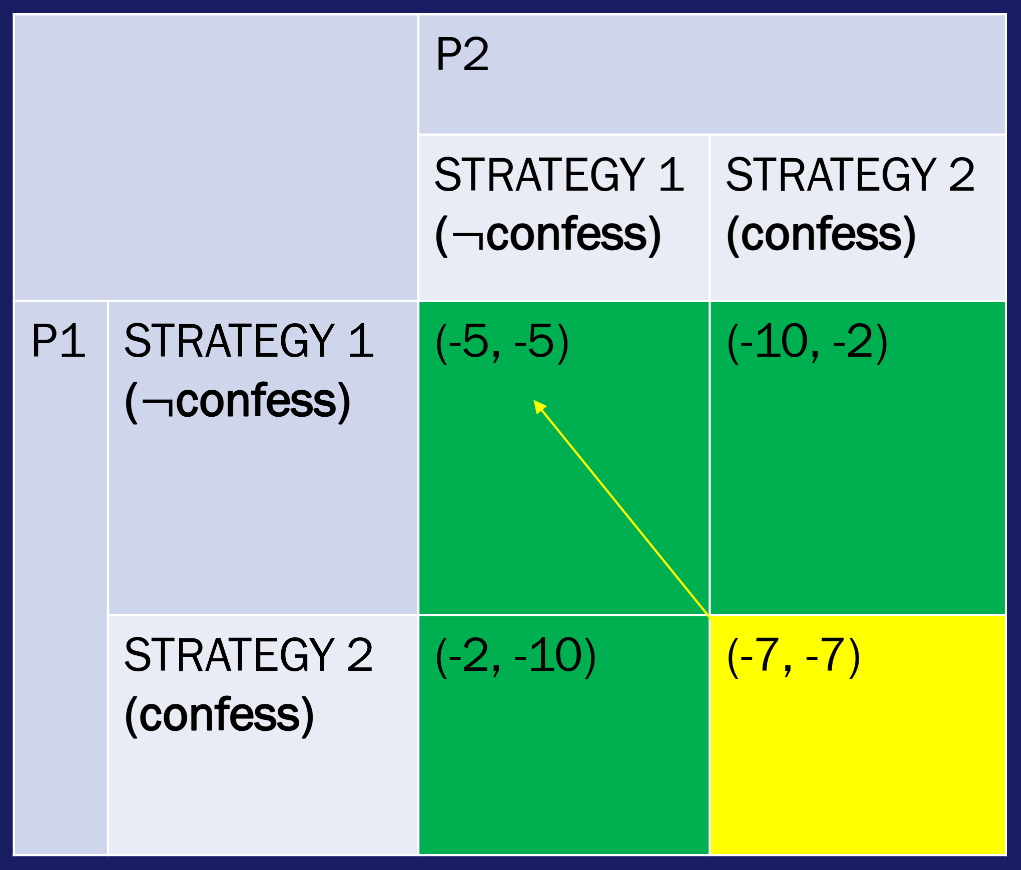
\includegraphics[width=.9\linewidth]{./images/prisoners-dilemma-utility-value-table.png}
\end{center}
\begin{itemize}
\item The cells coloured in \textbf{green} denotes a \textbf{Pareto-optimal} state of affairs.
\item The cell coloured in \textbf{yellow} denotes the \textbf{Nash equilibrium}.
\item If P1 and P2 are allowed to communicate and bargaining is \textbf{cost-free}, then P1 and P2 could agree to \textbf{cooperate} and not \textbf{confess}.
\item Hence, they could make a \textbf{Pareto-efficient move} indicated by the arrow (\(\rightarrow\))
\item The \textbf{Nash equilibrium} (coloured in \textbf{yellow}) arises because P1 and P2 behave as \textbf{straightforward maximisers}.
\item However, P1 and P2 have reasons to become \textbf{constrained maximisers}.
\end{itemize}

 \newpage
\subsection{Modification of rationality assumption}
\label{sec:orgff8c086}
\begin{itemize}
\item The original \textbf{rationality} assumption, which is \textbf{straightforward maximisation}, is as such:
It is \textbf{rational} to choose the course of action with the \textbf{maximum expected utility}.
\item The modified \textbf{rationality assumption}, is as such:
It is \textbf{rational} to be disposed to \textbf{constrained maximisation} and \textbf{cooperate} in \textbf{prisoner's dilemma-type scenarios}.
\end{itemize}
\subsection{Possible strategies for the game}
\label{sec:orgb12f1b9}
\begin{itemize}
\item Random, which is to choose to cooperate 50\% of the time.
\item Tit-for-tat (TFT), which is to choose to cooperate on the first move, and choose your opponent's last move as your next move.
\item Suspicious tit-for-tat (STFT), which is to choose to defect on the first move, and choose your opponent's last move as your next move.
\item Tit for two tats (TF2T), which is to choose to cooperate on the first two moves, then choose to cooperate as the next move, unless your opponent chooses to defect for 2 moves. When your opponent stops choosing to defect, then choose to cooperate.
\end{itemize}
\subsection{Axelrod's tournaments}
\label{sec:org394f010}
\begin{itemize}
\item The prisoner's dilemma was originally introduced as a \textbf{2-player game}, but it was later embedded by Axelrod into \textbf{round-robin tournaments}.
\item Each program was pitted against the rest of the field.
\item The aim of these tournaments was to learn about how to \textbf{choose effectively} in an \textbf{iterated prisoner's dilemma}.
\end{itemize}
\subsubsection{Properties of successful strategies}
\label{sec:orgcde1fa7}
\begin{center}
\begin{tabular}{|m{8em}|m{22em}|}
\hline
Property & Description\\
\hline
Be \textbf{nice} & Choose to cooperate on the first move. For example, Cooperative, TFT, TF2T.\\
\hline
Be \textbf{forgiving} & Do not immediately retaliate if your opponent chooses to defect in a move. For example, Cooperative, TF2T.\\
\hline
Be \textbf{prepared to retaliate if necessary}. & You must be prepared to choose to defect at some point if your opponent keeps choosing to defect. For example, TFT, STFT, TF2T\\
\hline
\end{tabular}
\end{center}
\begin{itemize}
\item What accounts for \textbf{tit-for-tat (TFT)'s} success is its combination of being \textbf{nice, retaliatory, forgiving,} and \textbf{clear}.
\item Its \textbf{niceness} prevents it from getting into \textbf{unnecessary trouble}.
\item Its \textbf{retaliation} discourages the other side from persisting whenever \textbf{defection} is tried.
\item Its \textbf{forgiveness} helps restore \textbf{mutual cooperation}.
\item Its \textbf{clarity} makes it intelligible to the other player, thereby eliciting \textbf{long-term cooperation}.
\end{itemize}

 \newpage
\subsection{Rapoport et al.'s objections to the Axelrod tournaments}
\label{sec:orgc824062}

\subsubsection{Objection 1}
\label{sec:org27e53e5}
The choice of \textbf{tournament format}:
\begin{itemize}
\item In a \textbf{knockout tournament}, top-ranked contestants at each stage progress to the next stage.
\item As the tournament continues, the number of competitors decreases.
\item In a \textbf{round-robin tournament}, each contestant competes with each of the others an equal number of times.
\item Axelrod chose the \textbf{single-stage round-robin format} for his tournaments.
\item He provided no \textbf{justification} for this choice of \textbf{tournament format}.
\item The \textbf{single-stage round-robin format} becomes \textbf{impractical} when the \textbf{number of contestants is large}, although this problem disappears when the tournament is run on a computer.
\end{itemize}
\subsubsection{Objection 2}
\label{sec:org291db92}
The choice of \textbf{criterion for determining success}:
\begin{itemize}
\item The \textbf{criterion for determining success} involved \textbf{maximising the number of points won across all dyadic interactions}.
\item Axelrod chose this \textbf{criterion of success}, but once again provided no \textbf{justification} for this choice of criterion for determining success.
\item Most of the programs were not designed to \textbf{maximise the total number of points}.
\item \textbf{Tit-for-tat (TFT)} can never win any particular \textbf{iterated prisoner's dilemma game}.
\item \textbf{Tit-for-tat (TFT)} can never achieve a \textbf{positive point difference} against any other program.
\end{itemize}
\subsubsection{Objection 3}
\label{sec:org7413d27}
The choice of \textbf{payoff structure}:
\begin{itemize}
\item The \(2 \times 2\) \textbf{prisoner's dilemma payoff matrix} had conventional values, where \(T\) denotes \textbf{sole defection}, \(R\) denotes \textbf{joint cooperation}, \(P\) denotes \textbf{joint defection}, and \(S\) denotes \textbf{sole cooperation}.
\item The values in this matrix are \((T, R, P, S) = (5, 3, 1, 0)\).
\item Axelrod chose this \textbf{payoff structure} but again provided no \textbf{justification} for this choice of \textbf{payoff structure}.
\end{itemize}
\subsubsection{Conclusion}
\label{sec:orgcee6fc9}
\begin{itemize}
\item Once the \textbf{2-player prisoner's dilemma} is embedded into a \textbf{tournament}, decisions have to be made about the \textbf{tournament format} (objection 1), \textbf{criteria for determining a winner} (objection 2), and \textbf{payoff structure} (objection 3).
\item However, Axelrod has provided no \textbf{justification} for his choices of \textbf{tournament format, criterion of determining success}, and \textbf{payoff structure}.
\item Hence, the policy recommendations about the effectiveness of \textbf{tit-for-tat (TFT)} should be qualified, i.e. the recommendations cannot be generalised.
\end{itemize}

 \newpage
\section{Ethics}
\label{sec:org5436c5a}
\textbf{Ethics} and \textbf{moral philosophy} are children nodes of the branch of \textbf{axiology}. Children nodes of \textbf{ethics} and \textbf{moral philosophy} include:
\begin{itemize}
\item \textbf{Metaethics, normative theory}, and \textbf{applied ethics}.
\end{itemize}

\begin{tikzpicture}[
    level 1/.style={level distance=3cm, sibling distance=3cm},
    level 2/.style={level distance=3cm, sibling distance=4cm},
    edge from parent/.style={draw,-}
]

% Root node
\node {Philosophy}
child {
    node {Axiology}
    child {
        node {Aesthetics}
    }
    child {
        node {Ethics}
        child {
            node {Metaethics}
        }
        child {
            node {Normative theory}
        }
        child {
            node {Applied ethics}
        }
    }
}
child {
    node {Metaphysics}
}
child {
    node {Epistemology}
}
child {
    node {Logic}
};
\end{tikzpicture}
\subsection{Branches of ethics}
\label{sec:org86b7404}
\begin{center}
\begin{tabularx}{\textwidth}{|X|X|X|}
\hline
Branch of ethics and moral philosophy & Central question & Elaboration\\
\hline
Metaethics (2\textsuperscript{nd}-order theory) & What is \textbf{morality}? & \textbf{Metaethics} is concerned with the \textbf{status, foundation, and scope} of \textbf{moral facts, values, properties, and terms}.\\
\hline
Normative theory (1\textsuperscript{st}-order theory) & What is \textbf{moral} (in \textbf{general})? & \textbf{Normative theory} is concerned with the articulation of \textbf{moral standards} and \textbf{rules of conduct}.\\
\hline
Applied ethics (praxis) & What is \textbf{moral} (in \textbf{specific, controversial issues})? & \textbf{Applied ethics} is concerned with the application of \textbf{philosophical theory} to \textbf{practical problems}.\\
\hline
\end{tabularx}
\end{center}
\subsection{Normative neutrality requirement}
\label{sec:org5e1b4b9}
\begin{center}
\begin{tabularx}{\textwidth}{|X|X|}
\hline
Branch of ethics and moral philosophy & Description\\
\hline
Normative theory (1\textsuperscript{st}-order theory) & There is NO \textbf{normative neutrality requirement}. \textbf{Normative theory} must have \textbf{substantive moral commitments}.\\
\hline
Metaethics (2\textsuperscript{nd}-order theory) & There is a \textbf{normative neutrality requirement}. \textbf{Metaethics} can have \textbf{classificatory moral commitments} but must avoid \textbf{substantive moral commitments}.\\
\hline
\end{tabularx}
\end{center}
 \newpage
\subsection{Forcehimes' collapse argument}
\label{sec:org51246cb}
\begin{itemize}
\item P1: There is a requirement for \textbf{normative neutrality} in \textbf{metaethics}.
\item P2: Such a \textbf{breach of normative neutrality} is \textbf{inevitable}.
\item Conclusion: Hence \textbf{metaethical theories (2\textsuperscript{nd}-order)} turn out to be \textbf{normative theories (1\textsuperscript{st}-order)} in disguise.
\end{itemize}
\subsection{Normative theory}
\label{sec:org42a0325}
The different approaches to \textbf{normative theory (1\textsuperscript{st}-order)} give rise to different \textbf{substantive moral commitments} and different \textbf{moral standards} and \textbf{rules of conduct}. The different approaches include:

\begin{center}
\begin{tabularx}{\textwidth}{|X|X|X|}
\hline
Degree of particularity & Approach & Elaboration\\
\hline
General & Approach 1: \textbf{High moral theory} & \textbf{Consequentialism} (camp 1), \textbf{deontology} (camp 2), \textbf{virtue ethics} (camp 3)\\
\hline
\(\downarrow\) & Approach 2: \textbf{Mid-level theory} & \textbf{Autonomy} (principle 1), \textbf{beneficence} (principle 2), \textbf{non-maleficence} (principle 3), \textbf{justice} (principle 4)\\
\hline
\(\downarrow\) & Approach 3: \textbf{Casuistry} or \textbf{case-based reasoning} & A \textbf{bottom-up approach} in which \textbf{moral principles} and \textbf{moral theories} emerge from case-based moral judgments.\\
\hline
Particular & Approach 4: \textbf{Narrative ethics} & We use stories to make sense of our experiences.\\
\hline
\end{tabularx}
\end{center}
 \newpage
\subsection{High moral theory}
\label{sec:org9ff6320}
From a set of \(n\) alternative courses of action, where \(i, n \in \mathbb{N}\) and \(i \in (0, n]\):
\begin{center}
\begin{tabularx}{\textwidth}{|X|X|}
\hline
Camp & Description\\
\hline
\textbf{Consequentialism} & \(\phi_i\)-ing is \textbf{morally right} if and only if it \textbf{maximises the good}, where the \textbf{good} is defined in terms of \textbf{some theory of the good T}.\\
\hline
\textbf{Deontology} & \(\phi_i\)-ing is \textbf{morally right} if and only if it has \textbf{intrinsic moral worth}.\\
\hline
\textbf{Virtue ethics} & \(\phi_i\)-ing is \textbf{morally right} if and only if it is the \textbf{best action} (in terms of \textbf{virtues and vices}) that a \textbf{virtuous agent} might perform in the circumstances.\\
\hline
\end{tabularx}
\end{center}
 \newpage
\subsubsection{Advantages}
\label{sec:org275888e}
\begin{center}
\begin{tabular}{|m{5em}|m{10em}|m{20em}|}
\hline
Advantage & Elaboration & Substantiation\\
\hline
Advantage 1 & \textbf{High moral theory} can provide \textbf{structured and systematic moral guidance}. & Camps 1 to 3 provide us with \textbf{moral standards} and \textbf{rules of conduct} for identifying the \textbf{morally appropriate action} (\(\phi_i\)-ing) from \(n\) alternative courses of action.\\
\hline
Advantage 2 & \textbf{High moral theory} can yield \textbf{moral standards} that can yield \textbf{moral standards} that can help us to achieve \textbf{consistency} and \textbf{coherence} in our moral lives. & For camp 1, there is the transitivity rule, which states if \(\phi_1\) is better than \(\phi_2\) and \(\phi_2\) is better than \(\phi_3\), then \(\phi_1\) must be better than \(\phi_3\).\\
 &  & For camp 2, there is the no-contradiction rule, which states that one and the same action \(\phi_i\) cannot be both \textbf{obligatory} and \textbf{impermissible}.\\
 &  & \\
 &  & For camp 3, there is the doctrine of the mean, which states that the \textbf{virtues} are a \textbf{mean} between the \textbf{vices of defect} and \textbf{excess}.\\
\hline
Advantage 3 & \textbf{High moral theory} often has the relevant tools and resources for \textbf{moral justification}. & Camp 1 delivers \textbf{evaluative claims} in terms of the \textbf{maximisation of the good}.\\
 &  & Camp 2 delivers \textbf{deontic verdicts} in terms of \textbf{duties, rights, and obligations.}\\
 &  & \\
 &  & Camp 3 delivers \textbf{virtue-ethical judgments} in terms of the \textbf{language of virtues and vices}.\\
\hline
\end{tabular}
\end{center}
 \newpage
\subsubsection{Disadvantages}
\label{sec:orga64dc56}
\begin{enumerate}
\item How do we choose a \textbf{moral theory} from the \textbf{competing alternatives}?
\begin{itemize}
\item Even if we do make a choice, how do we \textbf{justify} that choice?
\item Individuals with \textbf{different theoretical starting points} must still agree on a \textbf{similar set of principles}.
\item Hence, it has been argued that we should move to \textbf{mid-level theory} and a more \textbf{principle-based approach}.
\end{itemize}
\item How do we navigate \textbf{disagreement} within the ranks of each camp?
\begin{itemize}
\item For camp 1, \textbf{act} versus \textbf{rule based} forms of consequentialism, \textbf{maximising} versus \textbf{satisficing} forms of consequentialism.
\item For camp 2, \textbf{monistic} versus \textbf{pluralistic} forms of \textbf{deontology, agent} versus \textbf{patient-centred forms} of \textbf{deontology}.
\item For camp 3, \textbf{eudamimonist versus non-eudaimonist} forms of \textbf{virtue ethics}.
\end{itemize}
\item \textbf{High moral theory} may be too \textbf{ill-equipped} to deal with \textbf{practical decision-making at the concrete level}.
\begin{itemize}
\item When the \textbf{applied ethical problems} are \textbf{complex}, how likely is that \textbf{high moral theory} will be \textbf{sufficiently fine-grained} to generate responses?
\item For a move away from a \textbf{top-down approach} and toward a greater degree of \textbf{particularity}, it has been argued that we should favour \textbf{casuistry} or \textbf{case-based reasoning} or \textbf{narrative ethics} instead.
\end{itemize}
\end{enumerate}

 \newpage
\section{Consequentialism}
\label{sec:org250841f}
\begin{itemize}
\item From a set of \(n\) alternative courses of action, \(\phi_i\)-ing is \textbf{morally right} if and only if it \textbf{maximises the good}, where \(i, n \in \mathbb{N}, i \in (0, n]\), and the \textbf{good} is defined in terms of \textbf{some theory of the good T}.
\item The \textbf{core consequentialist commitment} is \textbf{maximising the good} (however the good might ultimately be defined).
\end{itemize}
\subsection{Consequentialist decision-making}
\label{sec:org1b7eb7a}
\begin{enumerate}
\item Compare the relative merits of \(n\) alternative courses of action \(\phi_1, \phi_2, \ldots, \phi_n\), where \(n \in \mathbb{N}\).
\item \textbf{Evaluate} these \(n\) courses of action in terms of whether they \textbf{maximise the good}.
\begin{itemize}
\item \(\phi_1\) \textbf{maximises the good}.
\item \(\phi_2\) does not \textbf{maximise the good}.
\end{itemize}
\item Arrive at the \textbf{decision outcome}. The \textbf{morally right} action is the one that \textbf{maximises the good} (for instance, \(\phi_1\)).
\end{enumerate}

 \newpage
\subsection{Theory of the Good}
\label{sec:orgf715a40}
\begin{itemize}
\item The \textbf{good to be maximised} is determined in terms of a \textbf{theory of the good T}.
\item However, there are \textbf{multiple theories of the good}.
\item Hence, one has not adopted any particular moral system in adopting \textbf{consequentialism} unless one says what the \textbf{good} is.
\end{itemize}

Candidate \textbf{theories of the good} include:
\begin{enumerate}
\item The \textbf{good} is defined as things which are \textbf{pink with yellow trimmings}.
\begin{itemize}
\item This is meant to be a joke.
\end{itemize}
\item The \textbf{good} is defined as things which ought to be \textbf{maximised}.
\begin{itemize}
\item This is possibly \textbf{trivial}, as the \textbf{core consequentialist commitment} becomes "that which \textbf{ought to be maximised, ought to be maximised}".
\end{itemize}
\item The \textbf{good} is defined as things that \textbf{facilitates self-interest}.
\item The \textbf{good} is defined as things that \textbf{facilitates human pleasure and happiness}.
\item The \textbf{good} is defined as that which is best understood as a \textbf{plurality of goods (happiness, justice, fairness, and so on)}.
\end{enumerate}

 \newpage
\subsection{Types of consequentialism}
\label{sec:org2c59c99}
Distinct types of \textbf{consequentialism} can be generated from \textbf{multiple theories of the good}:
\begin{center}
\begin{tabularx}{\textwidth}{|X|X|X|X|}
\hline
Type of consequentialism & Core consequentialist commitment & Theory of the good & Consequentialist outcome\\
\hline
\textbf{Ethical egoism} & The \textbf{good ought to be maximised}. & \textbf{Egoistic} theory of the good. & Select the action \(\phi_i\) that \textbf{maximises the good}.\\
 &  &  & \\
\textbf{Utilitarianism} &  & \textbf{Hedonistic} theory of the good. & \\
 &  &  & \\
\textbf{Pluralistic consequentialism and ideal utilitarianism} &  & \textbf{Pluralistic} theory of the good. & \\
\hline
\end{tabularx}
\end{center}
\subsection{Types of utilitarianism}
\label{sec:org3e8f60e}
For both \textbf{act} and \textbf{rule-based utilitarianism}, the \textbf{good} is what \textbf{facilitates human pleasure, happiness,} and \textbf{utility-based considerations}.
\begin{center}
\begin{tabularx}{\textwidth}{|X|X|X|}
\hline
Type of utilitarianism & Theory of the good & Description\\
\hline
\textbf{Act-based utilitarianism} & The \textbf{good} is defined as that which \textbf{facilitates human pleasure and happiness}. & \(\phi_i\)-ing is morally right if and only if it \textbf{maximises the good}.\\
 &  & \\
\textbf{Rule-based utilitarianism} &  & \(\phi_i\)-ing is morally right if and only if it is in accordance with a certain \textbf{set of rules R} that has been selected for its \textbf{good consequences}.\\
\hline
\end{tabularx}
\end{center}
\subsection{Hedonism}
\label{sec:orgc78a228}
\begin{itemize}
\item Both \textbf{act} and \textbf{rule-based utilitarianism} are characterised in terms of a \textbf{hedonistic} theory of the good.
\item Psychological hedonism: Only \textbf{pleasure (happiness)} or \textbf{pain (unhappiness)} motivates us.
\item Ethical hedonism: Only \textbf{pleasure (happiness)} has \textbf{value} and only \textbf{pain (unhappiness)} has \textbf{disvalue}.
\end{itemize}

According to the \textbf{greatest happiness principle}:
\begin{itemize}
\item Happiness is defined as \textbf{pleasure} and the \textbf{absence of pain} (\(\text{pleasure } \wedge \neg \text{ pain}\))
\item Unhappiness is defined as \textbf{pain} and the \textbf{privation of pleasure} (\(\text{pain } \wedge \neg \text{ pleasure}\))
\end{itemize}

Types of \textbf{ethical hedonism} include:
\begin{itemize}
\item \textbf{Quantitative hedonism}, which states that the \textbf{quantity of pleasure (happiness)} that matters.
\item \textbf{Qualitative hedonism}, which states that the \textbf{quality of pleasure (happiness)} that matters.
\end{itemize}
\subsection{Benthamite utilitarianism}
\label{sec:org1644719}
Benthamite utilitarianism is a \textbf{traditional account of utilitarianism} that can be characterised in terms of the following:
\begin{center}
\begin{tabularx}{\textwidth}{|X|X|X|}
\hline
Core consequentialist commitment & Hedonistic theory of the good & Consequentialist outcome\\
\hline
The good ought to be maximised. & Psychological hedonism & Select the action \(\phi_i\) that \textbf{maximises the good}.\\
 &  & \\
 & Ethical hedonism & \\
 &  & \\
 & Quantitative hedonism & \\
\hline
\end{tabularx}
\end{center}
\subsection{Hedonic calculus}
\label{sec:orga08bf07}
\begin{itemize}
\item Bethamite utilitarianism relies on a \textbf{hedonic calculus} or \textbf{felicific calculus}.
\item The \textbf{hedonic calculus} is an algorithm, formulated by Bentham, for \textbf{calculating the total quantity of pleasure (happiness)} that an action \(\phi_i\) is likely to cause.
\end{itemize}

The \textbf{variables} in the \textbf{hedonic calculus} include:
\begin{center}
\begin{tabular}{|m{5em}|m{25em}|}
\hline
Variable & Description\\
\hline
Intensity & How \textbf{strong} the \textbf{pleasure} or \textbf{pain} is.\\
\hline
Duration & How \textbf{long} the \textbf{pleasure} or \textbf{pain} lasts.\\
\hline
Probability & How \textbf{likely} the \textbf{pleasure} or \textbf{pain} is to be the result of \(\phi_i\)-ing.\\
\hline
Propinquity or remoteness & How close the sensation of \textbf{pleasure} or \textbf{pain} is to be the result of \(\phi_i\)-ing.\\
\hline
Fecundity & How likely \(\phi_i\) is to lead to further \textbf{pleasures} or \textbf{pains}.\\
\hline
Purity & How much \textbf{intermixture} there is between \textbf{pleasure} or \textbf{pain} and other sensations.\\
\hline
\end{tabular}
\end{center}
\subsection{Issues with quantitative hedonism}
\label{sec:orgfa838d7}
\begin{itemize}
\item Suppose that our choice is between \textbf{playing push-pin} (\(\phi_1\)) and \textbf{reading poetry} (\(\phi_2\)).
\item Suppose that the \textbf{total net utility value} of \(\phi_1\) equals the \textbf{total net utility value} of \(\phi_2\).
\item Quantitative hedonism states that only the \textbf{quantity of pleasure (happiness)} matters.
\item Hence, both \textbf{Benthamite utilitarianism} and its \textbf{machine-based implementation} \emph{Jeremy} will concur that \textbf{playing push-pin} (\(\phi_1\)) is as good as \textbf{reading poetry} (\(\phi_2\)).
\item There is a danger that \textbf{quantitative hedonism} might lead us to overvalue \textbf{bestial, unsophisticated, lower-quality, and debauched pleasures}.
\item However, human beings are able to distinguish between \textbf{lower-quality pursuits} such as \(\phi_1\) and \textbf{higher-quality intellectual pursuits} such as \(\phi_2\).
\end{itemize}
\subsubsection{Possible responses}
\label{sec:orgf12ee24}
\begin{center}
\begin{tabular}{|m{10em}|m{15em}|m{10em}|}
\hline
Response & Justification & Elaboration\\
\hline
Defend \textbf{quantitative hedonism}. & The \textbf{pleasures} associated with \textbf{reading poetry} (\(\phi_2\)) are \textbf{more probable, more durable, more fecund or more likely to lead to further pleasures,} and \textbf{purer} (unlikely to be mixed with pain). & The \textbf{quality of pleasure} can still be reduced to \textbf{quantitative considerations}. Hence, we can still retain \textbf{quantitative hedonism}.\\
\hline
Ditch \textbf{quantitative hedonism} in favour of \textbf{qualitative hedonism}. & \textbf{Qualitative hedonism} gives us automatic reasons to favour \textbf{higher-quality intellectual pursuits} such as \(\phi_2\) over \textbf{lower-quality pursuits} such as \(\phi_1\). & \\
\hline
\end{tabular}
\end{center}
 \newpage
\subsection{Qualitative hedonism}
\label{sec:orge23636a}
\begin{itemize}
\item The standard view of qualitative hedonism is that a \textbf{higher-quality pleasure} will be preferred to \textbf{any amount} of a \textbf{lower-quality pleasure}.
\item Let \(\phi_i\) denote \textbf{playing push-pin} and let \(\phi_2\) denote \textbf{reading poetry}.
\item Suppose that the total net utility value of \(\phi_1 = 5,000,000\) units and the total net utility value of \(\phi_2 = 1\) unit.

\[U(\phi_2) < U(\phi_1)\]

However, since a higher quality pleasure is preferred to a lower quality pleasure:
\[\phi_2 (\text{higher-quality}) \succ \phi_2 (\text{lower-quality})\]

\item We could postulate an \textbf{infinite superiority} of \textbf{higher-quality} over \textbf{lower-quality pleasures}.
\item However, this will reduce \textbf{qualitative} to \textbf{quantitative considerations}.
\item For the \textbf{non-standard view} of qualitative hedonism:
\begin{itemize}
\item \textbf{Qualitative hedonism} is not \textbf{quantitative hedonism} in disguise.
\item Rather, \textbf{quantity} and \textbf{quality} are two distinct properties of \textbf{pleasure}.
\item We may sometimes have to make \textbf{trade-offs} between a \textbf{lower-quantity} of a \textbf{higher-quality pleasure} and a \textbf{higher quantity} of a \textbf{lower-quality pleasure}.
\end{itemize}
\end{itemize}
\subsubsection{Dilemma regarding qualitative hedonism}
\label{sec:org1399493}
\begin{center}
\begin{tabularx}{\textwidth}{|X|X|}
\hline
Argumentative constituent & Elaboration\\
\hline
P1: Either the \textbf{quality of pleasure} contributes to the \textbf{total net utility value} in the same manner as the other \textbf{quantitative variables} in the \textbf{hedonic calculus}, or it does not. & The other \textbf{quantitative variables} in the \textbf{hedonic calculus} are \textbf{intensity, duration, probability, propinquity} or \textbf{remoteness, fecundity}, and \textbf{purity}.\\
\hline
P2 (horn 1): If the \textbf{quality of pleasure} contributes to the \textbf{total net utility value} in the same manner as the other \textbf{quantitative variables}, then \textbf{qualitative hedonism} will turn out to be \textbf{quantitative hedonism} in disguise. & This is the same problem confronting the \textbf{standard view of qualitative hedonism}, when it postulates an \textbf{infinite superiority} of \textbf{lower-quality pleasure} over \textbf{higher-quality pleasure}.\\
P3 (horn 2): If the \textbf{quality of pleasure} does not contribute to the \textbf{total net utility value} in the same manner as the other \textbf{quantitative variables}, the \textbf{qualitative hedonism} will be \textbf{inconsistent}. & According to \textbf{ethical hedonism}, only \textbf{pleasure (happiness)} has \textbf{value} and only \textbf{pain (unhappiness)} has \textbf{disvalue}. Hence, \textbf{ethical hedonism} implies \textbf{value monism}. However, \textbf{quality} appears to count as another \textbf{intrinsic good}.\\
\hline
C: Therefore, either \textbf{qualitative hedonism} will turn out to be \textbf{quantitative hedonism} in disguise (horn 1) or \textbf{qualitative hedonism} will be \textbf{inconsistent} (horn 2). & This is the \textbf{dilemma} confronting \textbf{qualitative hedonist}.\\
\hline
\end{tabularx}
\end{center}

 \newpage
\subsubsection{Schmidt-Petri's response to the dilemma}
\label{sec:orga625760}
We may sometimes have to make \textbf{trade-offs} between a \textbf{lower quantity} of a \textbf{higher-quality pleasure} and a \textbf{higher quantity} of a \textbf{lower-quality pleasure}.

\begin{enumerate}
\item Identify the \textbf{opponent}.
\begin{itemize}
\item The standard view of \textbf{qualitative hedonism} states that a \textbf{higher-quality pleasure} will \textbf{always} be chosen over a \textbf{lower-quality pleasure}, even when the \textbf{lower-quality pleasure} is available is a \textbf{lower quantity}.
\end{itemize}
\item Identify objections to the \textbf{standard view of qualitative hedonism}.
\begin{enumerate}
\item \textbf{Ambiguity} over the notion of "\textbf{quality}". Mill does not tell us what would correspond to the concept of "\textbf{quality}".
\item \textbf{Lack of clarity} about \textbf{experts}. We do not know how to tell who is an \textbf{expert} in the real world.
\end{enumerate}
\item Identify the \textbf{source material}, like Mill's Utilitarianism (Chapter 2, paragraph 5).
\item Distinguish between the \textbf{standard view} and the \textbf{non-standard view} relative to the \textbf{source material}.
\begin{itemize}
\item The \textbf{standard view} (incorrect): \(q \rightarrow p\)
If we are justified in saying that \(x\) is of a \textbf{higher quality} than \(y\), then some pleasure \(x\) is chosen over another pleasure \(y\) available in a \textbf{higher quantity}.
\item The \textbf{non-standard view} (correct): \(p \rightarrow q\)
If some pleasure \(x\) is chosen over another pleasure \(y\) available in a \textbf{higher quantity}, then we are justified in saying that \(x\) is of a \textbf{higher quality} than \(y\).
\end{itemize}
\end{enumerate}

 \newpage

\begin{enumerate}
\item Provide examples to support the \textbf{non-standard view}.
\begin{enumerate}
\item Example 1:
\begin{itemize}
\item Wine X (same quantity) \(\succ\) Wine Y (same quantity)
\item Wine X (slightly \textbf{lower-quantity}) \(\succ\) Wine Y (slightly \textbf{higher-quantity})
\item Appealing to the \textbf{higher quality} of Wine X is the most natural way for us to explain these \textbf{preference order relations}.
\end{itemize}
\begin{enumerate}
\item Example 2:
\begin{itemize}
\item Wine X (\textbf{lower-quantity}) \(\succ\) Wine Y (some \textbf{higher quantity} \(\le n\) units)
\item Wine Z (\textbf{lower-quantity}) \(\succ\) Wine Y (some \textbf{higher quantity} \(\le m\) units, where \(m > n\))
\end{itemize}
\item Example 3:
\begin{itemize}
\item Wine X (\textbf{1 glass}) \(\succ\) Wine Y (\textbf{ANY quantity})
\end{itemize}
\end{enumerate}
\end{enumerate}
\end{enumerate}

Therefore, the \textbf{standard view} is a \textbf{special case} of the \textbf{non-standard view}.

 \newpage
\subsection{Haydn and the oyster thought experiment}
\label{sec:orgb0d8ca6}
\begin{itemize}
\item Suppose you are a soul waiting to be allocated life on Earth.
\item The angel offers you a choice between:
\begin{itemize}
\item \(\phi_1\): Living the life of \textbf{Joseph Haydn}. Haydn composed some wonderful music, influenced the evolution of the symphony, was cheerful and popular, travelled, and enjoyed field sports.
\item \(\phi_2\): Living the life of an \textbf{oyster}. The \textbf{oyster's life} consists only of \textbf{mild sensual pleasure}. However, the \textbf{oyster's life} can be as long as you like.
\end{itemize}
\end{itemize}
\subsubsection{Bentham's hedonic calculus}
\label{sec:org26e4ac6}
The main part of the differences between the options in this thought experiment is the duration in which the \textbf{pain or pleasure lasts}.  \\

\begin{itemize}
\item Let \(m\) be the duration of the \textbf{oyster's life}.
\item Let \(n\) be a \textbf{threshold for sufficiency}.
\item \(m\) is a \textbf{sufficiently long duration} if and only if \(m \ge n\).
\item If the \textbf{oyster's life} is \textbf{sufficiently long} \(m \ge n\), then:
\[\phi_2 (\text{where the oyter's life is } m \text{ years }) \succ \phi_1 (\text{where Haydn's life is 77 years})\]
\end{itemize}

However, this cannot be right.

 \newpage
\subsubsection{Response}
\label{sec:orgbb66668}
\begin{itemize}
\item We could ditch \textbf{quantitative hedonism} in favour of \textbf{qualitative hedonism}.
\item \textbf{Qualitative hedonism} gives us automatic reasons to favour \textbf{higher-quality pleasure} (such as the life of Joseph Haydn) over \textbf{lower-quality pleasures} (such as an oyster's life).
\item However, according to the \textbf{non-standard view of qualitative hedonism}, we may sometimes have to make \textbf{trade-offs} between a \textbf{lower quantity of a higher-quality pleasure} and a \textbf{higher quantity of a lower-quality pleasure}.
\item If the \textbf{oyster's life} is \textbf{sufficiently long} \(m \ge n\), then a \textbf{trade-off} may have to be made.
\item Hence, \(\phi_2\) (where the oyster's life, though \textbf{lower-quality}, is \textbf{sufficiently long}) \(\succ \phi_1\) (where Haydn's life, though \textbf{higher-quality}, is \textbf{insufficiently long})
\end{itemize}
\subsection{Utility monster thought experiment}
\label{sec:org74f751a}
\begin{itemize}
\item Suppose that a \textbf{utility monster} is a hypothetical entity that is a \textbf{highly efficient consumer of resources}.
\item The \textbf{utility monster} gains vast amounts of \textbf{pleasure (happiness)} from very small quantities of a particular resource.
\item You have to choose between:
\begin{itemize}
\item \(\phi_1\): Satisfying the needs of the ordinary human beings.
\item \(\phi_2\): Satisfying the needs of the \textbf{utility monster}.
\end{itemize}
\item Given the existence of this \textbf{utility monster} and the \textbf{core consequentialist commitment} to \textbf{maximising the good}, it seems that we ought to neglect \(\phi_1\) in favour of \(\phi_2\).
\item However, this cannot be right.
\end{itemize}
\subsection{Against hedonism}
\label{sec:org3c574b4}
\begin{itemize}
\item \textbf{Consequentialists} will agree that:
\begin{itemize}
\item \(\phi_1\) (living the life of \textbf{Joseph Haydn}) \(\succ \phi_2\) (living the life of an \textbf{oyster}), however long the oyster's life might be.
\item \(\phi_1\) (satisfying the needs of ordinary human beings) \(\succ \phi_2\) (satisfying the needs of the \textbf{utility monster}), however \textbf{efficient} a \textbf{consumer of resources} the \textbf{utility monster} might be.
\end{itemize}
\item \textbf{Consequentialists} will typically not give up the \textbf{core consequentialist commitment} to \textbf{maximising the good}.
\item However, \textbf{consequentialists} may give up the \textbf{hedonistic} theory of the good.
\item The good is defined as that which \textbf{facilitates human pleasure and happiness}.
\item \textbf{Ethical hedonism} is a key element in the \textbf{hedonistic} theory of the good, as only \textbf{pleasure (happiness)} has \textbf{value} and only \textbf{pain (unhappiness)} has \textbf{disvalue}.
\end{itemize}

 \newpage
\subsubsection{Objections to ethical hedonism}
\label{sec:org4bb6f67}
\begin{center}
\begin{tabular}{|m{10em}|m{25em}|}
\hline
Objection & Elaboration\\
\hline
Deny \textbf{value monism} & \textbf{Ethical hedonism} implies \textbf{value monism}, where \(n\) denotes the number of \textbf{intrinsic goods}.\\
 & \textbf{Value monism} is when \(n = 1\), while \textbf{value pluralism} is when \(n > 1\).\\
 & However, we could maintain that while we ought to \textbf{maximise the good}, the \textbf{good} include far more than can be reduced to \textbf{pleasure (happiness)}. Hence, \textbf{pleasure (happiness)} is not the only \textbf{intrinsic good}. Other \textbf{intrinsic goods} include \textbf{beauty, friendship}, and so on. This leads to \textbf{value pluralism}.\\
\hline
Deny that certain \textbf{pleasure states} are \textbf{intrinsically good}. & A \textbf{sadist whipping her victim} or an \textbf{addict on drugs} might experience \textbf{pleasure (happiness)}. However, these \textbf{pleasure states} are not \textbf{intrinsically valuable}.\\
Problems with both \textbf{quantitative hedonism} and \textbf{qualitative hedonism}. & \textbf{Quantitative hedonism} might lead us to overvalue \textbf{bestial, unsophisticated, lower-quality}, and \textbf{debauched pleasures} (the push-pin versus poetry example).\\
 & At the same time, \textbf{qualitative hedonism} faces a \textbf{dilemma}. Either \textbf{qualitative hedonism} will turn out to be \textbf{quantitative hedonism} in disguise, or \textbf{qualitative hedonism} will be \textbf{inconsistent}.\\
\hline
Alternative \textbf{theories of the good} are superior to the \textbf{hedonistic} theory of the good. & \textbf{Pleasure} and \textbf{pain sensations}, inside the \textbf{heads of human beings}, are \textbf{difficult to measure}. By contrast, \textbf{well-being} can be defined in terms of \textbf{preference fulfilment} or \textbf{desire satisfaction}, giving rise to alternative \textbf{theories of the good}.\\
\hline
\end{tabular}
\end{center}

 \newpage
\subsubsection{Alternative theories of the good}
\label{sec:org6fb1763}
\begin{itemize}
\item Present desire satisfaction theory:
The \textbf{good} is defined as that which \textbf{facilitates the satisfaction of our current desires}. We also need a \textbf{fitting attitude account}, according to which what is \textbf{desired} is closely linked with what is \textbf{good}.
\item Comprehensive desire satisfaction theory:
The \textbf{good} is defined as that which \textbf{facilitates the satisfaction of desires over the course of our life}.
\item Informed desire satisfaction theory:
The \textbf{good} is defined as that which \textbf{facilitates the satisfaction of the desires we would have} if we were \textbf{fully informed of all the relevant facts}.
\item Objective list theory:
The \textbf{good} is defined as that which does not consist merely in either \textbf{pleasurable experience (hedonistic theory of the good)} or \textbf{desire satisfaction (desire satisfaction theory)}.
\end{itemize}
\subsubsection{Desire satisfaction theory}
\label{sec:org073620c}
\begin{itemize}
\item Desire satisfaction theory is also known as \textbf{preference fulfilment theory}.
\item We could get agents to \textbf{rank-order their preferences} and develop \textbf{utility functions} on their behalf.
\item \textbf{Preference utilitarianism} is based on \textbf{desire satisfaction theory}.
\item Relative to the agents' reported and \textbf{rank-ordered preferences} and these \textbf{utility functions}, we may be able to derive the following:
\begin{itemize}
\item \(U (\phi_1) > U (\phi_2)\), however long the oyster's life might be. Hence, \(\phi_1\) (living the life of \textbf{Joseph Haydn}) \(\succ \phi_2\) (living the life of an \textbf{oyster}).
\item \(U (\phi_1) > U (\phi_2)\), however \textbf{efficient} a \textbf{consumer of resources} the \textbf{utility monster} might be.
Hence, \(\phi_1\) (satisfying the needs of ordinary human beings) \(\succ \phi_2\) (satisfying the needs of the \textbf{utility monster}).
\end{itemize}
\end{itemize}
\subsubsection{Minimisation of the violation of rights}
\label{sec:org2d70ea4}
\begin{itemize}
\item The minimisation of the violation of rights could be identified as another relevant end for \textbf{consequentialism}.
\item Human beings have the \textbf{right to resources} that allow their needs to be satisfied.
\item Their \textbf{right to resources} function as \textbf{side constraints} on the pursuit of \textbf{good consequences}.
\item This gives rise to a \textbf{utilitarianism of rights}.
\item Therefore, \(\phi_1\) (satisfying the needs of ordinary human beings) \(\succ \phi_2\) (satisfying the needs of the \textbf{utility monster}).
\end{itemize}
\subsection{Formal definition of consequentialism}
\label{sec:org7baeed5}
\begin{itemize}
\item The term "consequentialism" was first introduced by G. E. M. Anscombe in "Modern moral philosophy" (1958).
\item According to consequentialism, only the \textbf{consequences of actions} matter, whereas the \textbf{intentions behind actions} are unimportant.
\end{itemize}

The elements of consequentialism include:
\begin{itemize}
\item A \textbf{core consequentialist commitment}, which is the \textbf{maximisation of the good}.
\item A \textbf{collection of theories of the good}.
\begin{itemize}
\item \textbf{Egoistic}: The good is defined as that which \textbf{facilitates self-interest}.
\item \textbf{Hedonistic}: The good is defined as that which \textbf{facilitates human pleasure and happiness}.
\item \textbf{Desire satisfaction theory}: The good is defined as that which \textbf{facilitates the satisfaction of our desire}.
\item \textbf{Objective list theory}: The good is defined as that which does not consist merely in either \textbf{pleasurable experiences (hedonistic theory of the good)} or \textbf{desire satisfaction (desire satisfaction theory)}.
\end{itemize}
\end{itemize}
\subsubsection{Semantics of consequentialism}
\label{sec:orgcfebd9e}
\begin{itemize}
\item The semantics of consequentialism can be interpreted in terms of a \textbf{semantics of possible worlds}.
\item To \textbf{maximise the good} is to make the \textbf{world}, the \textbf{sum of all things}, as \textbf{good as it can be}.
\item Alternatively, to \textbf{maximise the good} is to act to bring about the \textbf{best possible world} or all those worlds that can be brought about.
\item An \textbf{agent} (\(j, k\), and so on) is a \textbf{being capable of actions} that are \textbf{apt for moral evaluation}.
\item Each \textbf{action} \(\phi_i\) brings about a \textbf{possible world} \(w_i\).
\item Hence, an associated set of \textbf{possible worlds} \(w_1, w_2, \ldots, w_n\) is brought about by the alternative courses of action \(\phi_1, \phi_2, \ldots, \phi_n\).
\item \textbf{Possible worlds} \(w_1, w_2, \ldots, w_n\) are alternatives between which an \textbf{agent} \(j\) must choose.
\end{itemize}
\subsubsection{Definitions}
\label{sec:org8eca6d3}
\begin{itemize}
\item Let \(\Phi\) denote the set of alternative courses of action \(\phi_1, \phi_2, \ldots, \phi_n\).
\[\Phi = \{\phi_1, \phi_2, \ldots, \phi_n\}\]
\item Let \(W\) denote the set of \textbf{possible worlds} \(w_1, w_2, \ldots, w_n\), brought about by the actions in \(\Phi\).
\[W = \{w_1, w_2, \ldots, w_n\}\]
\item Let \(A\) denote the association of members of \(\Phi\) with their associated \textbf{possible worlds} in \(W\).
\[A = \{\phi_1 - w_1, \phi_2 - w_2, \ldots, \phi_n - w_2\}\]
\item Let \(<j, A>\) denote a \textbf{choice situation}, where \(j\) is the agent, \(A\) is the set of associations.
\item Let \(R\) denote a \textbf{rightness function} that assigns to each \textbf{choice situation} \(<j, A>\), a \textbf{subset of} \(A\).
\[<j, A> \overset{R}{\rightarrow} R_j (A)\]
\[\{\phi_1 - w_1, \phi_2 - w_2, \ldots, \phi_n - w_n\} \overset{R}{\rightarrow} \{\phi_1 - w_1 (\text{good}), \cancel{\phi_2 - w_2 (\neg \text{ good})}, \ldots, \cancel{\phi_n - w_n (\neg \text{ good})}\}\]
\end{itemize}
\subsubsection{Conditions}
\label{sec:org5dd4e76}
Let \(T\) denote a \textbf{theory of good}, representable in terms of a \textbf{complete order} \(\le\) on the \textbf{set \(W\) of all possible worlds}.

\begin{center}
\begin{tabularx}{\textwidth}{|X|X|X|}
\hline
Condition & Description & Formal representation\\
\hline
\textbf{Reflexivity} & \(x\) is \textbf{at least as good as itself}, according to \(T\). & \(x \le x\)\\
\hline
\textbf{Transitivity} & If \(y\) is \textbf{at least as good as} \(x\) and \(z\) is \textbf{at least as good as} \(y\), then \(z\) is \textbf{at least as good as} \(x\), according to \(T\). & \(((x \le y) \wedge (y \le z)) \rightarrow (x \le z)\)\\
\hline
\textbf{Completeness} & It is either the case that \(y\) is \textbf{at least as good as} \(x\) or that \(x\) is \textbf{at least as good as} \(y\), according to \(T\). & \((x \le y) \vee (y \le x)\)\\
\hline
\end{tabularx}
\end{center}

 \newpage
\subsubsection{Axioms of consequentialism}
\label{sec:org7294e75}
\begin{enumerate}
\item AN or agent neutrality. Consequentialism is \textbf{agent-neutral}.
For any two agents \(j\) and \(k\):
\[R_j (A) = R_k (A)\]

Essentially, it doesn't matter who or what the agent is, the right thing to do will always be the same.

\item NMD or \textbf{no moral dilemmas}. There are \textbf{no moral dilemmas} under \textbf{consequentialism}.
\[R_j (A) \ne \emptyset\]

\item DM or \textbf{dominance}. \(x\) \textbf{dominates} \(y\) under \textbf{consequentialism}.
\begin{itemize}
\item For any two possible worlds \(x\) and \(y\), an agent \(j\), and any two possible choice situations \(<j, A>\) and \(<j, B>\):
\item Suppose that \(\{x, y\} \subseteq A \cap B, x \in R_j (A)\) and \(y \notin R_j (A)\).
\[\therefore y \in R_j (B)\]
\item Essentially, what this axiom states is that once you have determined that one action is better than another action in a decision, the other action that you have rejected cannot be the best action in the next decision you make, because there is already a better action available.
\end{itemize}
\end{enumerate}

 \newpage
\subsubsection{Elements of consequentialism}
\label{sec:orgd224836}
\begin{enumerate}
\item The \textbf{agent} \(j\).
\item A set \(\Phi\) of alternative courses of action \(\phi_1, \phi_2, \ldots, \phi_n\).
\item A set \(W\) of \textbf{possible worlds} \(w_1, w_2, \ldots, w_n\) brought about by the actions in \(\Phi\).
\item An association \(A\) between members of \(\Phi\) and their associated \textbf{possible worlds} in \(W\).
\item The \textbf{choice situation} \(<j, A>\).
\item The \textbf{rightness function} \(R\).
\item The \textbf{theory of the good} \(T\), defined in terms of the following conditions:
\[\text{Reflexivity: } x \le x\]
\[\text{Transitivity: } ((x \le y) \wedge (y \le z)) \rightarrow (x \le z)\]
\[\text{Completeness: } (x \le y) \vee (y \le x)\]
\item The \textbf{axioms of consequentialism}:
\[(AN) \ R_j(A) = R_k (A)\]
\[(NMD) \ R_j(A) \ne \emptyset\]
(\(DM\)) Suppose that \(\{x, y\} \subseteq A \cap B, x \in R_j (A)\) and \(y \notin R_j (A)\):
\[\therefore y \notin R_j (B)\]
\end{enumerate}

 \newpage
\subsection{Violation of consequentialist axioms}
\label{sec:org3db930e}
It is possible for at least some of the \textbf{axioms of consequentialism} to be violated.
\subsubsection{Violating the agent neutrality axiom}
\label{sec:org1f16690}
\begin{itemize}
\item \textbf{Agent-relative consequentialism} combines the \textbf{core consequentialist commitment} (each agent ought to \textbf{maximise the good}) with an \textbf{agent-relative axiology}.
\item The correct evaluation of the \textbf{complete order} \(\le\) on the \textbf{set \(W\) of all possible worlds} may vary from agent to agent.
\item If there is an \textbf{agent-relative axiology}, then \(\Diamond (R_j (A) \ne R_k (A))\).
\item Hence, \(AN\) \textbf{(agent neutrality)} may be violated.
\end{itemize}
\subsubsection{Violating the no moral dilemmas axiom}
\label{sec:orgb446f4d}
\begin{itemize}
\item If the \textbf{theory of the good} \(T\) is defined in terms of \textbf{completeness}, then for any two possible worlds \(x\) and \(y\), either \(x > y, x = y\) or \(y > x\).
\item The \textbf{good} must be represented by a \textbf{complete order} \(\le\).
\item This rules out \textbf{incommensurability}.
\item However, if \(\le\) is \textbf{incomplete}, then we could allow for \textbf{incommensurability between at least some possible worlds}.
\item Therefore, this would allow \textbf{moral dilemmas} within \textbf{consequentialism}.
\[R_j (A) = \emptyset\]
\item Therefore, NMD (\textbf{no moral dilemmas}) will be violated.
\item The possibility of \textbf{moral dilemmas} within \textbf{consequentialism} might require us to drop NMD.
\end{itemize}

 \newpage
\subsubsection{Violating the dominance axiom}
\label{sec:orgf51eb62}
\begin{itemize}
\item \textbf{Satisficing consequentialism} relaxes the \textbf{maximising element} in \textbf{consequentialism}.
\item According to \textbf{satisficing theories}, it is sometimes permissible to do something than is \textbf{worse than the best}, provided that it is \textbf{good enough}.
\item Hence, DM (\textbf{dominance}) will be violated.
\item Relative to the choice situations \(<j, B>\), the \textbf{satisficing threshold} is \textbf{sufficiently low}.
\item Therefore, \(x \in R_j (B)\) and \(y \in R_j (B)\) (both \(x\) and \(y\) are \textbf{good enough}).
\item Hence, \(x\) does not \textbf{dominate} \(y\).
\item DM (\textbf{dominance}) will be violated.
\end{itemize}

 \newpage
\subsection{Driver's strategy}
\label{sec:org67b247f}

\subsubsection{Move 1}
\label{sec:orgc497d52}
Identify objections to \textbf{consequentialism} raised by the \textbf{standard feminist view}.
\begin{itemize}
\item Objection 1: \textbf{Consequentialism} is \textbf{too demanding} of the individual.
\item Objection 2: \textbf{Consequentialism} is \textbf{neglectful of an agent's special obligations} to family and friends.
\end{itemize}
\subsubsection{Move 2}
\label{sec:orgc0d7bbf}
Identify the problems of \textbf{consequentialism}.
\begin{itemize}
\item Problem 1: \textbf{Impartiality} - we should \textbf{maximise the good, impartially considered}.
\item Problem 2: \textbf{Demandingness} - \textbf{consequentialism} appears to make \textbf{theoretically unlimited demands}.
\end{itemize}
\subsubsection{Move 3}
\label{sec:org87594da}
Introduce \textbf{conceptual distinctions}.
\begin{itemize}
\item The angel of the house \textbf{is partial to her domestic sphere} and \textbf{self-sacrificing}.
\item The angel of the world \textbf{is impartial} and \textbf{self-sacrificing}.
\item \textbf{Moral self-sufficiency}: There is a concern with promoting an \textbf{internalist standard of moral worth}, as our wills are sufficient to ground our moral worth, and we do not need to look externally for the source of this value.
\item \textbf{Ethical self-sufficiency}: There is a concern with promoting a \textbf{risk aversion standard}.
\begin{itemize}
\item The best life needs to incorporate a \textbf{respect for personal space}.
\item There is space in \textbf{ethics} for \textbf{self-perfection, personal projects, goals,} and \textbf{aspirations}.
\end{itemize}
\end{itemize}
\subsubsection{Move 4}
\label{sec:orga8faab0}
Articulate a \textbf{sophisticated consequentialism}.
\begin{itemize}
\item The aim here is to avoid the \textbf{angel of the world} and \textbf{ethical self-sufficiency} (Schopenhauer's ideal).
\item Introduce further \textbf{conceptual distinctions} between:
\begin{enumerate}
\item A \textbf{decision procedure} and a \textbf{criterion for rightness of actions}.
A \textbf{decision procedure} may interfere with the actual production of the good, as determined by some \textbf{criterion of rightness}.
\item \textbf{Truth conditions} and \textbf{acceptance conditions}.
We could hold that \textbf{consequentialism} is true, although we do not accept it in certain areas of our life.
\end{enumerate}
\end{itemize}
\subsubsection{Move 5}
\label{sec:org81e67b5}
Anticipate objections to \textbf{sophisticated consequentialism}.
\begin{itemize}
\item Objection: \textbf{Moral schizophrenia}.
\item Response: \textbf{Moral schizophrenia} does not speak against the \textbf{truth} of a theory.
\item It merely shows that the theory is \textbf{difficult to apply} as a \textbf{decision procedure}.
\item A \textbf{theory} may be \textbf{true} yet difficult to apply.
\item The \textbf{impartial good} will be promoted if the \textbf{angel of the world} cultivates \textbf{special relationships} and becomes less of an all-encompassing angel.
\item Therefore, we now have a \textbf{norm of partiality}, which means we ought to show preference for our family and friends.
\end{itemize}
\subsubsection{Conclusion}
\label{sec:orgd53207c}
As a \textbf{sophisticated consequentialist}, one can be \textbf{both a consequentialist and a feminist}. One can be responsive to both \textbf{feminist concerns about partiality} and the \textbf{demands of morality}.

 \newpage
\section{Deontology}
\label{sec:org7c32ff7}

\subsection{Hiroshima and Nagasaki}
\label{sec:org6075e12}
\begin{itemize}
\item Should the atomic bombings of Hiroshima and Nagasaki have been carried out or not?
\item Let \(\phi\) denote the action of carrying out the atomic bombings of Hiroshima and Nagasaki.
\item Since \(\phi\)-ing has brought about the \textbf{best possible consequences} (the end of WWII and world peace), \(\phi\)-ing should have been carried out.
\end{itemize}
\subsubsection{Argument in favour of \(\phi\)-ing}
\label{sec:orgb1194ff}
\begin{itemize}
\item Only the \textbf{consequences of actions} matter, whereas the \textbf{intentions behind actions} are unimportant.
\item There are no \textbf{side constraints} under \textbf{consequentialism}.
\item \(\phi\)-ing would be \textbf{morally right} due to the \textbf{maximisation of the good}.
\item Therefore, the \textbf{evaluative claim} under \textbf{consequentialism} is that we ought to \(\phi\).
\end{itemize}
\subsubsection{Argument not in favour of \(\phi\)-ing}
\label{sec:orga4a2df5}
\begin{itemize}
\item \textbf{Side constraints} exist under \textbf{deontology} \(\phi\)-ing would be \textbf{morally wrong} due to the \textbf{violation} of certain \textbf{side constraints}.
\item Therefore, the \textbf{deontic verdict} under \textbf{deontology} is that we ought not to \(\phi\).
\end{itemize}

 \newpage
\subsection{Textbook view}
\label{sec:org76cf380}
According to the \textbf{textbook view}:
\begin{itemize}
\item \textbf{Consequentialism} is an \textbf{agent-neutral theory}, whereas \textbf{deontology} is an \textbf{agent-relative theory}.
\item The \textbf{textbook view} has also been describe as the \textbf{standard method} for drawing the distinction between \textbf{consequentialism} and \textbf{deontology}.
\end{itemize}

The \textbf{textbook view} implies the following:
\begin{center}
\begin{tabularx}{\textwidth}{|X|X|}
\hline
Deontology & Consequentialism\\
\hline
Deontology may give \textbf{different agents} \(j, k\), etc. \textbf{different aims}. & \textbf{Consequentialism} gives \textbf{different agents} \(j, k\), etc. the \textbf{same aim}: select the action \(\phi_i\) that \textbf{maximises the good}.\\
\hline
Deontology introduces \textbf{agent-relative side constraints}. & \textbf{Consequentialism} does not observe any \textbf{agent-relative side constraints}.\\
\hline
\(\Diamond(R_j (A) \ne R_k (A))\) with an \textbf{agent-relative axiology}. Hence, AN (\textbf{agent neutrality}) may be violated. & (AN or \textbf{agent neutrality}) \(R_j (A) = R_k (A)\)\\
 & AN is an \textbf{axiom} under \textbf{consequentialism}.\\
\hline
We can give \textbf{higher weight} to our interests, projects, and concerns. & We must give \textbf{equal weight} to our interests and the interests of others.\\
\hline
We might have certain \textbf{special obligations} (for instance, \textbf{obligations} that parents have to their own children), not shared by other agents. & We ought to be \textbf{impartial}.\\
\hline
We end up with \textbf{agent-relative reasons for action}. & We end with \textbf{agent-neutral reasons for action}.\\
\hline
\end{tabularx}
\end{center}

 \newpage
\subsubsection{Exceptions to the textbook view}
\label{sec:org8cce1f4}
\begin{enumerate}
\item \textbf{Ethical egoism}
\begin{itemize}
\item \textbf{Ethical egoism} is supported by an \textbf{egoistic} theory of the good.
\item The \textbf{good} is defined that which \textbf{facilitates self-interest}.
\item Since what counts as \textbf{self-interest} may differ from agent to agent, \textbf{ethical egoism} may give \textbf{different agents} \(j, k\), etc. \textbf{different aims}.
\item Therefore, \textbf{ethical egoism} is an \textbf{agent-relative} version of \textbf{consequentialism}.
\end{itemize}
\item \textbf{Agent-neutral deontology}
\begin{itemize}
\item \textbf{Agent-neutral deontology} is an \textbf{agent-neutral} version of \textbf{deontology}.
\item \textbf{Agent-neutral deontology} gives \textbf{different agents} \(j, k\), etc. the \textbf{same aim}.
\end{itemize}
\end{enumerate}
\subsection{Mafia scenario}
\label{sec:orgfb2d92e}
\begin{itemize}
\item Suppose that the mafia are credibly threatening to kill two strangers unless you \textbf{kill a third stranger}.
\item Let \(\phi\) denote the action of \textbf{killing the third stranger}.
\item Should we ought to \(\phi\) or \(\neg \phi\)?
\end{itemize}

\begin{center}
\begin{tabularx}{\textwidth}{|X|X|}
\hline
Deontology & Consequentialism\\
\hline
The \textbf{deontic verdict} is that we ought not to \(\neg \phi\). & The \textbf{evaluative claim} is that we ought to \(\phi\).\\
\hline
\textbf{Justification} for \textbf{deontic verdict}. & \textbf{Justification} for \textbf{evaluative claim}.\\
\textbf{Side constraints} exists that \textbf{prohibit killing} as a \textbf{morally wrong} type of action. & We ought to \textbf{minimise the number of bad occurrences}.\\
\hline
\end{tabularx}
\end{center}

 \newpage
\subsection{Side constraints}
\label{sec:org54a83c9}
There are two types of \textbf{side constraints}.
\begin{center}
\begin{tabularx}{\textwidth}{|X|X|X|}
\hline
Type of side constraint & Description & Implication\\
\hline
An \textbf{agent-relative side constraint}. & Each agent should ensure that \textbf{she does not kill}, even if to \textbf{prevent more killings by others}. & \textbf{Agent-relative side constraints} might give an agent a \textbf{special concern} with her own killings.\\
\hline
An \textbf{agent-neutral side constraint}. & Each agent should ensure that \textbf{no one kills}, even if to \textbf{prevent more killings by others}. & \textbf{Agent-neutral side constraints} gives \textbf{different agents} \(j, k\), etc. the \textbf{same aim}.\\
 & \textbf{Agent-neutral side constraints} may require everyone to \textbf{share a moral vision}. & \\
\hline
\end{tabularx}
\end{center}
\subsection{The right and the good}
\label{sec:orgc0a0969}
\begin{itemize}
\item The \textbf{textbook view} uses the \textbf{agent-neutral and agent-relative} distinction to distinguish between \textbf{conseuqentialism} and \textbf{deontology}.
\item Another popular approach to distinguishing between \textbf{consequentialism} and \textbf{deontology} involves an appeal to the \textbf{right or good} distinction:
\end{itemize}
\begin{center}
\begin{tabularx}{\textwidth}{|X|X|}
\hline
Deontology & Consequentialism\\
\hline
The \textbf{right} is \textbf{prior} to the \textbf{good}. & The \textbf{good} is \textbf{prior} to the \textbf{right}.\\
\hline
\textbf{Deontology} delivers \textbf{deontic verdicts} in terms of \textbf{what is right}. & \textbf{Consequentialism} delivers \textbf{evaluative claims} in terms of \textbf{what is good}.\\
If an action \(\phi\) is \textbf{morally impermissible}, then it is \textbf{not right}, no matter how much \textbf{good} might be produced by \(\phi\)-ing. & \\
\hline
\end{tabularx}
\end{center}
\subsection{Action and intention}
\label{sec:org2b92be8}
We can distinguish between different types of \textbf{deontology} in terms of the \textbf{action or intention} distinction and the \textbf{agent versus patient} distinction:

\begin{center}
\begin{tabularx}{\textwidth}{|X|X|}
\hline
Types of deontology & Description\\
\hline
Action-based deontology & The \textbf{right action} is \textbf{prior} to the \textbf{good consequences}.\\
\hline
Intention-based deontology & The \textbf{right intention} is \textbf{prior} to the \textbf{good consequences}.\\
\hline
Action and intention-based deontology & The \textbf{right action} and \textbf{right intention} are \textbf{prior} to the \textbf{good consequences}.\\
\hline
Agent-centred deontology & The primary concern is with the \textbf{duties of the agent}.\\
\hline
Patient-centred deontology & The primary concern is with the \textbf{rights of the patient}. The \textbf{patient} has a \textbf{right against being used} as a mere \textbf{means for producing good consequences} without her consent.\\
\hline
\end{tabularx}
\end{center}
\subsection{Doctrine of double effect}
\label{sec:org61a45da}
\begin{itemize}
\item \textbf{Intention-based deontology} is supported by the \textbf{doctrine of double effect}.
\item The doctrine of double effect states that it is \textbf{morally impermissible} for us to \textbf{intend evil} (for instance, the \textbf{killing or torturing of innocents}).
\end{itemize}

Possible objections to the \textbf{doctrine of double effect}:
\begin{enumerate}
\item The distinctions between \textbf{intending, foreseeing, risking, predicting} and \textbf{causing and allowing} are \textbf{conceptually incoherent}.
\item The distinctions invite \textbf{manipulation} and can be \textbf{exploited}.
\end{enumerate}

 \newpage
\subsection{Avoision}
\label{sec:orgc6e1c1b}
\begin{itemize}
\item Suppose that there is a \textbf{moral prohibition} against \(\phi_1\)-ing.
\item However, \(\phi_2\)-ing allows an agent to \textbf{bypass, circumvent,} or \textbf{duck this moral prohibition}.
\item Does \(\phi_2\)-ing count as a \textbf{morally permissible avoidance} of the \textbf{moral prohibition}?
\item Does \(\phi_2\)-ing count as a \textbf{morally impermissible evasion} of the \textbf{moral prohibitions}?
\item This type of \textbf{manipulation} in the legal domain has been termed \textbf{avoision}.
\item The distinctions between \textbf{intending, foreseeing, risking, predicting} and \textbf{causing and allowing} could give rise to a \textbf{moral} version of \textbf{avoision}.
\end{itemize}
\subsection{Trolley dilemma}
\label{sec:org0606477}
\begin{itemize}
\item According to the \textbf{trolley dilemma}, a \textbf{runaway tram or trolley} is on course to run over and \textbf{kill five people on the main track}.
\item However, you can intervene, \textbf{pull the lever}, and divert the runaway tram or trolley to a \textbf{side track, killing just one person}.
\item You have to choose between:
\begin{itemize}
\item \(\phi\): \textbf{Pulling the lever} and \textbf{killing the one person on the side track} to \textbf{save the five people on the main track}.
\item \(\neg \phi\): \textbf{Refraining from pulling the lever} and \textbf{letting the five people on the main track die}.
\end{itemize}
\item Should you \textbf{pull the lever} and \textbf{kill one} to \textbf{save five} \(\phi\) or \textbf{refrain from doing so} \(\neg \phi\)?
\end{itemize}

 \newpage
\subsubsection{Positions}
\label{sec:orge710f68}
\begin{itemize}
\item \textbf{Consequentialism} recommends \textbf{pulling the lever} and \textbf{killing one to save five} (\(\phi\)).
\begin{itemize}
\item \(\phi\)-ing will \textbf{minimise the number of bad occurrences}.
\item We ought to \textbf{minimise the number of bad occurrences}.
\item Hence, we ought to \(\phi\).
\end{itemize}
\item \textbf{Action-based deontology} recommends \textbf{refraining from pulling the lever} (\(\neg \phi\)).
\begin{itemize}
\item \(\phi\)-ing is a \textbf{morally impermissible action}.
\item \(\neg \phi\)-ing is a \textbf{morally permissible action}.
\item Hence, we ought to \(\neg \phi\).
\end{itemize}
\item \textbf{Intention-based deontology} recommends two different actions.
\begin{enumerate}
\item \textbf{Pull the lever} and \textbf{kill one to save five} (\(\phi\)).
\begin{itemize}
\item \(\phi\)-ing may be accompanied by the \textbf{intention of saving five}.
\item We merely \textbf{risk, foresee, or predict} that \(\phi\)-ing will have the consequence of one innocent person being killed.
\item Hence, we ought to \(\phi\).
\end{itemize}
\item \textbf{Refrain from pulling the lever} (\(\neg \phi\)).
\begin{itemize}
\item \(\phi\)-ing may be accompanied by the \textbf{intention of killing one innocent person}.
\item We should not \textbf{intend evil}.
\item Hence, we ought to \(\neg \phi\).
\end{itemize}
\end{enumerate}
\item \textbf{Patient-centred deontology} recommends \textbf{refraining from pulling the lever} (\(\neg \phi\))
\begin{itemize}
\item \textbf{That one person on the side track} has a \textbf{right against being used} as a mere \textbf{means for producing good consequences} without their consent.
\item Hence, we ought to \(\neg \phi\).
\end{itemize}
\end{itemize}
\subsection{Siamese twins}
\label{sec:org2df6865}
\begin{itemize}
\item Suppose that \textbf{Siamese twins} are conjoined such that \textbf{both will die} unless the \textbf{organs of one are given to the other} via an operation that kills the first.
\item You have to choose between:
\begin{itemize}
\item (\(\phi\)): Performing the \textbf{life-saving operation}.
\item (\(\neg \phi\)): \textbf{Refraining from} performing the \textbf{life-saving operation}.
\end{itemize}
\end{itemize}
\subsubsection{Positions}
\label{sec:org0b5902e}
\begin{itemize}
\item \textbf{Intention-based deontology} recommends \textbf{performing the life-saving operation} (\(\phi\))
\begin{itemize}
\item We \textbf{intend} to save the first twin in a \textbf{life-saving operation}.
\item We do not \textbf{intend} but merely \textbf{foresee} the death of the second twin in that operation.
\item Hence, we ought to \(\phi\), justified by the use of \textbf{foreseeing and intending} distinction.
\end{itemize}
\item \textbf{Action-based deontology} recommends \textbf{performing the life-saving operation} (\(\phi\))
\begin{itemize}
\item We \textbf{cause the first twin to be saved} in a \textbf{life-saving operation}.
\item We do not \textbf{cause} but merely \textbf{allow} the death of the second twin in that operation.
\item Hence, we ought to \(\phi\), justified by the use of the \textbf{causing and allowing} distinction.
\end{itemize}
\item \textbf{Patient-centred deontology} recommends \textbf{refraining from performing the operation} (\(\neg \phi\))
\begin{itemize}
\item Each twin has a \textbf{right against being used} as a mere \textbf{means for producing good consequences} without her consent.
\item Hence, we ought to \(\neg \phi\).
\end{itemize}
\end{itemize}
\subsection{Divine command theory}
\label{sec:org877dadf}
\begin{itemize}
\item \textbf{Divine command theory} is a form of \textbf{deontology}.
\item In \textbf{divine command theory}, the \textbf{side constraints} are provided by the \textbf{divine commands of God}.
\item Examples of \textbf{divine commands} and religious precepts supporting the \textbf{side constraint against murder}:
\begin{enumerate}
\item Thou shalt not kill, from Exodus 20:13. This is one of the \textbf{10 Commandments} in \textbf{Judaism} and \textbf{Christianity}.
\item I undertake the precept to \textbf{refrain from destroying living creatures}. This is one of the \textbf{five precepts in Buddhism}.
\item One ought to \textbf{avoid harming (or desiring to harm) any living being} in thought, word or deed. This is the \textbf{doctrine of Ahimsa} in \textbf{Jainism, Hinduism,} and \textbf{Buddhism}.
\end{enumerate}
\item These religious commandments, precepts, and doctrines \textbf{prohibit killing} as a \textbf{morally wrong} type of action and function as \textbf{side constraints}.
\end{itemize}
\subsubsection{Definition}
\label{sec:org04b67f0}
\begin{itemize}
\item \textbf{Divine command theory} is the view according to which:
\begin{itemize}
\item \textbf{Morality} is somehow dependent upon \textbf{God}.
\item \textbf{Moral obligation} consists in \textbf{obedience to God's commands}.
\end{itemize}
\item \textbf{Divine command theory} consists of at least some of the following claims:
\begin{enumerate}
\item \textbf{Morality} is the ultimately based on the \textbf{commands of God}.
\item \textbf{Morality} is ultimately based on the \textbf{character of God}.
\item \textbf{Moral obligations} are identical with \textbf{divine commands}.
\item \textbf{Moral obligations} are created by \textbf{divine commands}.
\end{enumerate}
\item \textbf{Divine command theory} has to address the \textbf{Euthyphro dilemma}.
\end{itemize}
\subsubsection{Euthyphro dilemma}
\label{sec:org854e616}
\begin{itemize}
\item Socrates' original question to Euthyphro:
Is the \textbf{pious} loved by the gods because it is pious, or is it pious because it is loved by the gods?
\item Revised version of Socrates' question:
Is an action \textbf{divinely commanded} by God because it is \textbf{morally right}, or is an action \textbf{morally right} because it is \textbf{divinely commanded} by God?
\item Horn 1: An \textbf{action} is \textbf{divinely commanded} by God because it is \textbf{morally right}.
Problems associated with this horn:
\begin{enumerate}
\item God would no longer be the \textbf{author of morality}. Rather, God would be merely a \textbf{being capable of recognising right and wrong}.
\item God would not be the \textbf{sovereign of morality}. Rather, God would be a mere \textbf{subject of morality}.
\end{enumerate}
\item Horn 2: An \textbf{action} is \textbf{morally right} because it is \textbf{divinely commanded} by God.
Problems associated with this horn:
\begin{enumerate}
\item Nothing guarantees that what God would \textbf{divinely command} would be in accordance with what \textbf{morality} would prescribe. If God commands us to do something \textbf{morally reprehensible}, then the \textbf{morally reprehensible} action would be \textbf{morally right}.
\item The \textbf{foundations of morality} become \textbf{arbitrary}. \textbf{Morally reprehensible actions} can become \textbf{morally obligatory} if \textbf{divinely commanded} by God.
\end{enumerate}
\end{itemize}

 \newpage
\subsection{Modified divine command theory}
\label{sec:orgc459d87}
\begin{itemize}
\item According to \textbf{standard divine command theory}:
"\(\phi\)-ing is \textbf{morally wrong}" means "\(\phi\)-ing is contrary to the \textbf{divine commands} of God."
\item According to the \textbf{modified divine command theory}:
"\(\phi\)-ing is \textbf{morally wrong}" means "\(\phi\)-ing is contrary to the \textbf{divine commands} of a \textbf{loving} God."
\item \textbf{Modified divine command theory} holds that God has a particular character.
\item God has the character of \textbf{loving his human creatures}.
\item Therefore, while it is \textbf{logically possible} for God to command \textbf{morally reprehensible} action, it is not actually something that God would do, given his character.
\end{itemize}
\subsubsection{How it fixes the issues with Euthyphro's dilemma}
\label{sec:org25c951a}
Horn 1:
\begin{itemize}
\item God is the \textbf{subject} rather than the \textbf{sovereign of morality}.
\item Under \textbf{modified divine command theory}, God remains the \textbf{source of morality}.
\item \textbf{Morality} is grounded in the \textbf{loving} character of God.
\end{itemize}

Horn 2:
\begin{itemize}
\item The \textbf{foundations of morality} become \textbf{arbitrary}.
\item Under \textbf{modified divine command theory}, not any \textbf{divine command} goes.
\item \textbf{Divine commands} remain rooted in the unchanging \textbf{loving} and \textbf{omnibenevolent} character of God.
\end{itemize}

\textbf{Standard divine command theory} is pierced by either \textbf{horn 1} and \textbf{horn 2}. However, the \textbf{modified divine command theory} appears to fare better against the \textbf{Euthyphro dilemma}.
\subsection{Plato}
\label{sec:org534f71b}

\subsubsection{Context}
\label{sec:org4819e3e}
\begin{itemize}
\item \textbf{Socrates} is being accused of \textbf{corrupting the youth of Athens}.
\item \textbf{Socrates} is about to be put to trial and thereafter found \textbf{guilty} of both:
\begin{enumerate}
\item \textbf{Corrupting the minds of the youth of Athens}.
\item \textbf{Impiety} ("not believing in the Gods of the state").
\end{enumerate}
\item \textbf{Euthyphro} is \textbf{prosecuting his father} for \textbf{murder}.
\item Both Socrates and Euthyphro try to arrive at a definition of \textbf{piety} or \textbf{holiness}.
\item Euthyphro's modified definition of \textbf{piety} or \textbf{holiness} (suggested by Socrates):
\begin{itemize}
\item Holy is defined as what all the gods love.
\item Unholy is defined as what all the gods hate.
\item \(\neg\) (Holy \(\vee\) Unholy) is defined as what some gods love and some other gods hate.
\item (Holy \(\vee\) Unholy) is defined as what some gods love and some other gods hate.
\end{itemize}
\end{itemize}
\subsubsection{The Euthyphro's dilemma}
\label{sec:org1e4f748}
\begin{itemize}
\item The \textbf{Euthyphro dilemma}:
Is the \textbf{holy} loved by the gods because it is holy? Or is it holy because it is loved by the gods?
\item Revised version of the \textbf{Euthyphro dilemma}:
Is what is \textbf{morally good} commanded by God or the gods because it is \textbf{morally good}? Or is it \textbf{morally good} because it is commanded by God or the gods?
\item \textbf{Species-genus} distinction:
\begin{itemize}
\item The \textbf{species} is a \textbf{part} of the \textbf{genus (whole)}.
\item \textbf{Reverence (species)} is a \textbf{part} of \textbf{fear (genus)}.
\item \textbf{Piety} or \textbf{holiness (species)} is a \textbf{part} of \textbf{justice (genus)}.
\end{itemize}
\item According to \textbf{Euthyphro}:
The part of \textbf{justice (genus)} that is \textbf{holy (species)} involves \textbf{ministering to} (looking after or \textbf{taking care} of) the gods.
\end{itemize}
\subsubsection{Socrates' argument by analogy}
\label{sec:orgfbbeaa7}
\begin{center}
\begin{tabularx}{\textwidth}{|X|X|}
\hline
Source & Target\\
\hline
We \textbf{take care of animals}. & The part of \textbf{justice (genus)} that is \textbf{holy (species)} involves \textbf{taking care of the gods} (Euthyphro's claims).\\
\hline
\textbf{Taking care of horses, dogs}, and \textbf{cattle} in horsetraining, huntsmanship, and herdsmanship \textbf{benefits and improves horses, dogs}, and \textbf{cattle}. You make these animals \textbf{better}. & You do not make the gods \textbf{better} when you do something \textbf{pious} or \textbf{holy}.\\
\hline
\end{tabularx}
\end{center}

Therefore, Euthyphro's claims are problematic.
\subsubsection{Conclusion}
\label{sec:org0ded945}
\begin{itemize}
\item The \textbf{pious} or \textbf{holy} is in fact \textbf{something other than what is acceptable to the gods}.
\item Something's being acceptable to the gods is merely an \textbf{attribute} of \textbf{piety} and not part of its \textbf{defining characteristics}.
\item Therefore, Socrates still does not have a \textbf{definition of piety} or \textbf{holiness}.
\end{itemize}

 \newpage
\subsection{Secular deontology}
\label{sec:org54f2892}
Deontology may be \textbf{religious} or \textbf{secular} in nature.
\subsubsection{Religious form of deontology}
\label{sec:orgcb2d7fd}
\begin{itemize}
\item All \textbf{duties and obligations} are generated by \textbf{religious precepts, commandments}, and \textbf{doctrines}.
\item An example is \textbf{divine command theory}, which has \textbf{religious precepts, commandments}, and \textbf{doctrines} that are of \textbf{divine origin}.
\end{itemize}
\subsubsection{Secular form of deontology}
\label{sec:org731f7a0}
\begin{itemize}
\item All \textbf{duties and obligations} are generated by \textbf{secular principles}.
\item An example is \textbf{deontological monism}, where all \textbf{duties and obligations} are generated by a \textbf{single secular principle}.
\item Another example is \textbf{deontological pluralism}, where all \textbf{duties and obligations} are generated by \textbf{multiple secular principles}.
\end{itemize}
\subsection{Kantian deontology}
\label{sec:org2f7a1df}
\begin{itemize}
\item \textbf{Kantian deontology} is an example of a \textbf{secular} form of \textbf{deontology}.
\item All \textbf{duties and obligations} are generated by a \textbf{single secular principle}.
\item This \textbf{single secular principle} is known as the \textbf{categorical imperative}.
\end{itemize}

 \newpage
\subsubsection{Types of imperatives}
\label{sec:orgc4e6798}
\begin{enumerate}
\item Hypothetical imperative
\begin{itemize}
\item A \textbf{command} that applies to us \textbf{conditionally}.
\item \textbf{Hypothetical imperatives} contain conditional clauses that can be explicit or elided.
\item \textbf{Hypothetical imperatives} require us to exercise our wills in a certain way, given that we have \textbf{antecedently} willed a particular end.
\item An example is, "If you are happy, and you know it, clap your hands".
\end{itemize}
\item Categorical imperative
\begin{itemize}
\item A \textbf{command} that applies to us \textbf{unconditionally}, regardless of what we might want.
\item \textbf{Categorical imperatives} do not have any \textbf{conditional clauses}, that can be \textbf{explicit} or \textbf{elided}.
\item An example is, "Thou shalt not kill."
\end{itemize}
\end{enumerate}
\subsubsection{Categorical imperative formulations}
\label{sec:orgcca19b3}
\begin{enumerate}
\item The \textbf{universal law of nature} formula.
\item The \textbf{humanity} formula.
\item The \textbf{autonomy} formula.
\item The \textbf{kingdom of ends} formula.
\end{enumerate}

Formulations 1 to 4 are supposed to be \textbf{equivalent}, hence \textbf{Kantian deontology} is also an example of \textbf{deontology monism}.

 \newpage
\subsubsection{Universal law of nature formula}
\label{sec:orgcac97c6}
\begin{itemize}
\item The \textbf{universal law of nature} states:  \\
Act only in accordance with that \textbf{maxim} that you can at the same time will that it become \textbf{universal law}.
\item Decision procedure associated with the \textbf{universal law of nature} formula:
\begin{enumerate}
\item Consider a particular action \(\phi\) (for instance, stealing).
\item Determine a \textbf{maxim} governing \(\phi\) (for instance, I will steal for pleasure).
\item \textbf{Universalise} that \textbf{maxim} and consider the implications (for instance, everyone ought to steal for pleasure).
\item Consider whether the \textbf{universalised} version of the \textbf{maxim} is \textbf{contradiction-free}. Could the \textbf{universalised} version of the \textbf{maxim} function as a \textbf{law of nature}?
\end{enumerate}
\item Example:
Suppose I borrow money from you and promise to return the amount eventually, but I know that I will not return the amount.
\end{itemize}

 \newpage
\subsubsection{Detailed steps for the universal law of nature formula}
\label{sec:org01af94b}
\begin{enumerate}
\item Consider a particular action \(\phi\).
\begin{itemize}
\item Here, \(\phi\)-ing denotes the action of \textbf{borrowing money and promising to repay}, despite knowing that \textbf{this will never be done}.
\end{itemize}
\item Determine a \textbf{maxim} governing \(\phi\).
\begin{itemize}
\item Maxim: Whenever I am low on cash, I will \textbf{borrow money and promise to repay}, despite knowing that \textbf{this will never be done}.
\end{itemize}
\item \textbf{Universalise} that \textbf{maxim} and consider the implications.
\begin{itemize}
\item \textbf{Universalised} version of maxim: Whenever anyone is low on cash, she ought to \textbf{borrow money and promise to repay}, despite knowing that \textbf{this will never be done}.
\item However, if this deceit is \textbf{universalised}, there will be no institution of \textbf{promising} to begin with.
\end{itemize}
\item Consider whether the \textbf{universalised} version of the \textbf{maxim} is \textbf{contradiction-free}.
\begin{itemize}
\item A \textbf{contradiction} arises, as we cannot \textbf{make promises} if there is no institution of \textbf{promising} to begin with.
\item Therefore, I will be unable to make my \textbf{promise} to begin with.
\end{itemize}
\end{enumerate}
\subsubsection{Humanity formula}
\label{sec:org6827ba7}
\begin{itemize}
\item The \textbf{humanity} formula states:  \\
Act in such a way that you always treat \textbf{humanity}, whether in your own person or in the person of any other, never simply as a \textbf{means}, but always at the same time as an \textbf{end}.
\item Implications:
\begin{itemize}
\item We ought to \textbf{respect the humanity in persons}.
\item We ought to refrain from treating persons as \textbf{mere instruments}.
\end{itemize}
\end{itemize}
\subsubsection{Autonomy formula}
\label{sec:org9f58ad1}
\begin{itemize}
\item The \textbf{autonomy} formula:
Act in such a way that your \textbf{will} can regard itself at the same time as \textbf{making universal law through its maxims}.
\item Implications:
\begin{itemize}
\item We ought to act as \textbf{universal lawgivers} or \textbf{legislators}.
\item We ought to consider whether our intended maxims are worthy of our status as \textbf{shapers of the world}.
\item As \textbf{rational agents}, we are the very \textbf{source of the authority} for the \textbf{moral laws} that bind us.
\end{itemize}
\end{itemize}
\subsubsection{Kingdom of ends formula}
\label{sec:orgad7bc41}
\begin{itemize}
\item The \textbf{kingdom of ends} formula:
Act in accordance with the \textbf{maxims} of a member giving \textbf{universal laws} for a \textbf{merely possible kingdom of ends}.
\item Implications:
\begin{itemize}
\item We ought to consider whether our intended maxims will earn \textbf{acceptance} by a \textbf{community of fully rational agents} in a \textbf{kingdom of ends}.
\item Just as \textbf{human beings} are \textbf{ends in themselves}, we are also a \textbf{kingdom of ends} or a \textbf{moral community}.
\end{itemize}
\end{itemize}

 \newpage
\subsection{Organ transplant thought experiment}
\label{sec:org0b412b1}
\begin{itemize}
\item Suppose that \textbf{five mortally ill patients} are at a hospital.
\item They will soon die without an organ transplant.
\item Each of these patients requires a different organ to be transplanted (for instance, a \textbf{heart} for the first patient, a \textbf{kidney} for the second patient, a \textbf{liver} for the third patient, and so on).
\item At the same time, a \textbf{sixth healthy patient} is undergoing a routine check-up at the same hospital.
\item The only medical means of \textbf{saving the five mortally ill patients} would be to \textbf{kill the sixth healthy patient} and transplant his healthy organs into the five other patients.
\item You have to choose between:
\begin{itemize}
\item (\(\phi\)): Killing the \textbf{one healthy patient} to \textbf{save the five mortally ill patients}.
\item (\(\neg \phi\)): Refraining from killing the \textbf{one healthy patient}, even at the cost of the \textbf{five mortally ill patients} dying.
\end{itemize}
\item Should you kill the \textbf{one healthy patient} to \textbf{save the five mortally ill patients} (\(\phi\)) or refrain from doing so (\(\neg \phi\))?
\end{itemize}
\subsubsection{Consequentialist position}
\label{sec:orgd7fe944}
\begin{itemize}
\item Consequentialism recommends \textbf{killing the one healthy patient} to \textbf{save the five mortally ill patients} (\(\phi\)).
\item Justification:
\begin{itemize}
\item \(\phi\)-ing will \textbf{maximise the good}.
\item Certain \textbf{theories of the good} might require us to \(\phi\).
\item Therefore, we ought to \(\phi\).
\end{itemize}
\end{itemize}

 \newpage
\subsubsection{Deontological position}
\label{sec:org6b6f6cc}
\begin{itemize}
\item The deontological position recommends refraining from killing the one healthy patient \(\neg \phi\).
\item Justification:
\begin{itemize}
\item \(\phi\)-ing is a \textbf{morally impermissible action}.
\item \(\neg \phi\)-ing is a \textbf{morally permissible action}.
\item The \textbf{humanity} formula introduces \textbf{side constraints} against \(\phi\)-ing.
\item \(\phi\)-ing requires that you treat the \textbf{sixth healthy patient} as a mere \textbf{means} or \textbf{conduit} for \textbf{five useful and life-saving organs}.
\item Hence, we ought to \(\neg \phi\).
\end{itemize}
\end{itemize}
\subsubsection{Permissivity}
\label{sec:org81cd890}
For consequentialism:
\begin{itemize}
\item The \textbf{evaluative claim} of \textbf{consequentialism}:
\begin{itemize}
\item \(\phi\)-ing is not merely \textbf{morally permissible}.
\item \(\phi\)-ing is also \textbf{morally obligatory}, we ought to \textbf{maximise the good (core consequentialist commitment)}
\item Hence, \textbf{consequentialism} appears to be \textbf{overpermissive}.
\end{itemize}
\end{itemize}

For deontology:
\begin{itemize}
\item The \textbf{deontic verdict} of \textbf{deontology}:
\begin{itemize}
\item \(\phi\)-ing is \textbf{morally impermissible}.
\item \(\phi\)-ing violates certain \textbf{side constraints} (including the \textbf{humanity} formula)
\item Hence, \textbf{deontology} is not \textbf{overpermissive}.
\end{itemize}
\end{itemize}

Note that the \textbf{organ transplant} thought experiment and the \textbf{trolley dilemma}:
\begin{itemize}
\item (Trolley dilemma): \textbf{Pull the lever} and \textbf{kill one} to \textbf{save five} (\(\phi\)) or \textbf{refrain from doing so} (\(\neg \phi\))?
\item (Organ transplant): \textbf{Kill the sixth healthy patient} to \textbf{save five} \(\phi\) or \textbf{refrain from doing so} (\(\neg \phi\))?
\end{itemize}
\subsection{Rossian deontology}
\label{sec:org87ee88a}
\begin{itemize}
\item \textbf{Kantian deontology} is an example of \textbf{deontological monism}.
\item All \textbf{duties and obligations} are generated by a \textbf{single secular principle}.
\item By contrast, \textbf{Rossian deontology} is an example of \textbf{deontological pluralism}.
\item All \textbf{duties and obligations} are generated by \textbf{multiple secular principle}.
\item Furthermore, these \textbf{multiple secular principles} cannot be reduced to a \textbf{single master or mistress principle}.
\end{itemize}
\subsubsection{Principles}
\label{sec:orge42c201}
\begin{itemize}
\item Fidelity:
We have a duty to \textbf{keep our promises}.
\item Reparation:
We have a duty to \textbf{right our previous wrongs}.
\item Gratitude:
We have a duty to \textbf{return services} to those from whom we have accepted benefits in the past.
\item Beneficence:
We have a duty to promote a \textbf{maximum of aggregate good}.
\item Nonmaleficence:
We have a duty to \textbf{refrain from harming others}.
\end{itemize}

 \newpage
\subsubsection{Prima facie duties}
\label{sec:org228898d}
\begin{itemize}
\item \textbf{Rossian principles} specify \textbf{aspects of a situation} that \textbf{count morally} in favour of an action \(\phi\).
\item For instance, an action \(\phi\) that allows us to \textbf{right our previous wrongs (reparation) counts morally} in favour of \(\phi\)-ing.
\item \textbf{Rossian principles} yield \textbf{prima facie duties}.
\item However, \textbf{prima facie duties} can be \textbf{outweighed} by other \textbf{prima facie duties}.
\item Furthermore, \textbf{moral dilemmas} may arise when \textbf{prima facie duties conflict} with each other.
\item What the agent ought to choose under \textbf{Rossian deontology} is that action \(\phi_i\):
Of all those possible for the agent in the circumstances, that has the \textbf{greatest balance of prima facie rightness}, in those respects in which they are \textbf{prima facie right}, over their \textbf{prima facie wrongness}, in those respects in which they are \textbf{prima facie wrong}.
\end{itemize}
\subsubsection{Conflicts between prima facie duties}
\label{sec:orgb21e245}
\begin{itemize}
\item \textbf{Rossian deontology} maintains that any \textbf{conflict between prima facie duties} in a particular situation can be resolved by relying on \textbf{intuition}.
\item We can rely on our \textbf{crystal-clear intuitions} in both \textbf{mathematics} and \textbf{ethics} to build up all we can know about the \textbf{nature of numbers} and the \textbf{nature of duty}.
\item Our \textbf{mathematical knowledge} and our \textbf{moral knowledge} are \textbf{self-evident}.
\item When we assume that \(AB\) and \(CD\) are parallel, i.e. \(AB \parallel CD\), then \(AB\) and \(CD\) do not meet except at infinity in a Euclidean plane is self-evident by \textbf{mathematical intuition}.
\item \(\neg Pp\), where \(p\) denotes the action of \textbf{genocide} is \textbf{self-evident} by \textbf{moral intuition}.
\item The \textbf{actual duty} is what the agent is left with after she has weighed up all the \textbf{conflicting prima facie duties} in the manner prescribed by Ross.
\end{itemize}
\subsubsection{Issues with intuition to resolve conflicts}
\label{sec:orgf801137}
\begin{enumerate}
\item How do we even identify the \textbf{prima facie duties} that are involved in a particular situation?
\item What are the \textbf{criteria} according to which we \textbf{rank and compare prima facie duties}, in order to arrive at the \textbf{greatest balance of prima facie rightness over prima facie wrongness} (as prescribed by Ross) that will guide us to our \textbf{actual duty}?
\item What if our \textbf{intuitions} are \textbf{wrong or misguided}?
\end{enumerate}
\subsection{W.D.}
\label{sec:org5246401}
\begin{itemize}
\item W.D. is a machine-based implementation of \textbf{Rossian deontology}.
\item Jeremy and W.D. are important developments in the domain of \textbf{machine ethics}.
\item \textbf{Machine ethics} is broadly concerned with ensuring that the \textbf{behaviour of machines} is \textbf{ethically acceptable}.
\item The \textbf{relations} to be learnt by W.D. are represented as \textbf{first-order horn clauses} of the form:
\[H \leftarrow (L_1 \wedge L_2 \wedge \cdots \wedge L_n)\]

Where:
\begin{itemize}
\item \(H\) is a positive literal \(H\)
\item \(\leftarrow\) means implication
\item \((L_1 \wedge L_2 \wedge \cdots \wedge L_n)\) is a universally quantified conjunctions of positive literals \(L_i\)
\end{itemize}
\item W.D. uses \textbf{inductive logic programming} to learn the \textbf{supersedes relation}:
\[\text{supersedes}(\phi_1, \phi_2)\]

This means that action \(\phi_1\) is preferred over action \(\phi_2\) in a particular situation.
\end{itemize}
\subsubsection{Favours relation}
\label{sec:orgd795110}
The \textbf{favours relation} is a \textbf{4-ary relation} that is used as a \textbf{specifying operation} to aid the supersedes relation:
\[\text{favours}(1 \text{ or } 2, D_{\phi_1}, D_{\phi_2}, R)\]

Where:
\begin{itemize}
\item \(1\) or \(2\) signifies in which action's favour (\(\phi_1\) or \(\phi_2\)), a given \textbf{prima facie duty} lies. The possible values are \(\{1, 2\}\).
\item \(D_{\phi_1}\) signifies \(\phi_1\)'s \textbf{intensity value} for a particular \textbf{prima facie duty}. The possible values are \(\{-2, -1, 0, +1, +2\}\).
\item \(D_{\phi_2}\) signifies \(\phi_2\)'s \textbf{intensity value} for a particular \textbf{prima facie duty}. The possible values are \(\{-2, -1, 0, +1, +2\}\).
\item \(R\) specifies \textbf{how far apart} the \textbf{intensity values} of these \textbf{prima facie duties} can be. The possible values are \(\{1, 2, 3, 4\}\).
\end{itemize}

For any two actions \(\phi_1\) and \(\phi_2\):
\[\text{favours}(1, D_{\phi_1}, D_{\phi_2}, R) \leftarrow D_{\phi_1} - D_{\phi_2} \ge R\]
\[\text{or}\]
\[\text{favours}(2, D_{\phi_2}, D_{\phi_1}, R) \leftarrow (D_{\phi_2} - D_{\phi_2} \ge 0) \wedge (D_{\phi_2} - D_{\phi_2} \le R)\]

\begin{itemize}
\item W.D. begins by making a \textbf{hypothesis} about how the \textbf{favours relation} supports the \textbf{supersedes relation}.
\begin{itemize}
\item Completeness: A \textbf{hypothesis} is \textbf{complete} if and only if it covers \textbf{all the positive cases}.
\item Consistency: A \textbf{hypothesis} is \textbf{consistent} if and only if it covers \textbf{no negative cases}.
\end{itemize}
\item Therefore, a hypothesis could be:
\begin{itemize}
\item (Complete \(\wedge\) consistent): \textbf{All positive} and \textbf{no negative} cases covered.
\item (Complete \(\wedge\) \(\neg\) consistent): \textbf{All positive} and \textbf{at least some negative cases} covered.
\item (\(\neg\) Complete \(\wedge\) consistent): \textbf{Not all positive} and \textbf{no negative cases} covered.
\item (\(\neg\) Complete \(\wedge\) \(\neg\) consistent): \textbf{Not all positive} and \textbf{at least some negative cases} covered.
\end{itemize}
\end{itemize}
\subsubsection{Input information}
\label{sec:org4dd21d8}
\begin{enumerate}
\item The name of \textbf{action} \(\phi_1\).
\item A rough estimate of the \textbf{intensity} of each of the \textbf{prima facie duties} satisfied or violated by this action \(\phi_i\).
\begin{itemize}
\item -2 means a \textbf{serious violation} of duty
\item -1 means a \textbf{less serious violation} of duty
\item 0 means a duty is \textbf{neither satisfied nor violated}
\item +1 means a \textbf{minimal satisfaction} of duty
\item +2 means a \textbf{maximal satisfaction} of duty
\end{itemize}
\end{enumerate}

 \newpage
\subsubsection{Machine learning procedure}
\label{sec:orgf3df93b}
\begin{enumerate}
\item When the data entry is complete, W.D. consults its \textbf{current version of the supersedes relation}.
\begin{itemize}
\item W.D. determines whether there is any action \(\phi_i\) that \textbf{supersedes} all other actions.
\item Formal representation:
\[\text{supersedes}(\phi_1, \phi_2) \veebar \text{supersedes}(\phi_2 , \phi_1)\]
\[\text{supersedes}(\phi_1, \phi_2) \veebar \text{supersedes}(\phi_2 , \phi_1)\]
\[\text{supersedes}(\phi_1, \phi_2) \veebar \text{supersedes}(\phi_2 , \phi_1)\]
\[\vdots\]
\end{itemize}
\item If this action \(\phi_i\) is discovered, then it will be \textbf{output} as the \textbf{correct action} to perform.
Formal representation:
\begin{displaymath}
\text{supersedes}(\phi_1, \phi_i) \leftarrow \begin{cases}
\text{supersedes}(\phi_1, \phi_2) \\
\text{supersedes}(\phi_1, \phi_3) \\
\text{supersedes}(\phi_1, \phi_4) \\
\text{supersedes}(\phi_1, \phi_5) \\
\hspace*{3.5em} \vdots \\
\text{supersedes}(\phi_1, \phi_n) \\
\end{cases}
\end{displaymath}
\item If no such action exists, then W.D. will seek the \textbf{intuitively correct action} from the user.
\item The new information from the user is combined with the \textbf{input case} to form a \textbf{new training example}. This \textbf{training example} is used to refine the \textbf{current hypothesis}.
\item The aim of \textbf{training W.D.} is to allow it to learn a \textbf{new hypothesis} that is a \textbf{complete and consistent}, relative to all \textbf{input cases}.
\end{enumerate}

 \newpage
\subsubsection{Example 1}
\label{sec:orgf3a3c22}
\begin{itemize}
\item We could either \textbf{refrain from killing an innocent person} and \textbf{using his heart to save another person's life} (\(\phi_1\)) or \textbf{kill that person to use his heart to save the other person's life} (\(\phi_2\)).
\item The \textbf{intuitively correct} response is \(\phi_1\):
\begin{itemize}
\item For \(\phi_1\):
\begin{itemize}
\item \(\text{Beneficence}_{\phi_1} = - 2\)
\item \(\text{Nonmaleficence}_{\phi_1} = + 2\)
\end{itemize}
\item For \(\phi_2\):
\begin{itemize}
\item \(\text{Beneficence}_{\phi_2} = + 2\)
\item \(\text{Nonmaleficence}_{\phi_2} = - 2\)
\end{itemize}
\end{itemize}
\item W.D. starts with the \textbf{most general hypothesis}: \(\text{supersedes}(\phi_1, \phi_2)\).
\item The list of \textbf{least specific specialisations} for the \textbf{favours relation} includes:
\begin{itemize}
\item \(\text{favours}(1, \text{fidelity}_{\phi_1}, \text{fidelity}_{\phi_2}, 1)\)
\item \(\text{favours}(1, \text{reparation}_{\phi_1}, \text{reparation}_{\phi_2}, 1)\)
\item \(\text{favours}(1, \text{gratitude}_{\phi_1}, \text{gratitude}_{\phi_2}, 1)\)
\item \(\text{favours}(1, \text{beneficence}_{\phi_1}, \text{beneficence}_{\phi_2}, 1)\)
\item \(\text{favours}(1, \text{nonmaleficence}_{\phi_1}, \text{nonmaleficence}_{\phi_2}, 1)\)
\end{itemize}
\item Hence:
\[\text{beneficence}_{\phi_2} - \text{beneficence}_{\phi_1} = 2 - (-2) = 4\]
\[\text{nonmaleficence}_{\phi_1} - \text{nonmaleficence}_{\phi_2} = 2 - (-2) = 4\]
\item Therefore, only one \textbf{favours relation} covers example 1:
\[\text{favours}(1, \text{nonmaleficence}_{\phi_1}, \text{nonmaleficence}_{\phi_2}, 1)\]
\item Therefore, the \textbf{hypothesis} that is \textbf{complete} and \textbf{consistent} through example 1 will be:
\[\text{supersedes}(\phi_1, \phi_2) \leftarrow \text{favours}(1, \text{nonmaleficence}_{\phi_1}, \text{nonmaleficence}_{\phi_2}, 1)\]
\end{itemize}
\subsubsection{Example 2}
\label{sec:org885eb0f}
\begin{itemize}
\item We could either ask a \textbf{slightly squeamish person} to \textbf{give some of her blood}, when no other suitable donors are available, to \textbf{save another person's life} (\(\phi_1\)) or refrain from asking and \textbf{let the person die} (\(\phi_2\)).
\item The \textbf{intuitively correct} response is \(\phi_1\):
\begin{itemize}
\item For \(\phi_1\):
\begin{itemize}
\item \(\text{Beneficence}_{\phi_1} = + 2\)
\item \(\text{Nonmaleficence}_{\phi_1} = - 1\)
\end{itemize}
\item For \(\phi_2\):
\begin{itemize}
\item \(\text{Beneficence}_{\phi_2} = - 2\)
\item \(\text{Nonmaleficence}_{\phi_2} = + 1\)
\end{itemize}
\end{itemize}
\end{itemize}
\subsubsection{Initiating training}
\label{sec:orge953937}
In example 1:
\(\phi_1\) (\textbf{positive case}), \(\phi_2\) (\textbf{negative case})
\[\text{beneficence}_{\phi_2} - \text{beneficence}_{\phi_1} = 2 - (-2) = 4\]
\[\text{nonmaleficence}_{\phi_1} - \text{nonmaleficence}_{\phi_2} = 2 - (-2) = 4\]

In example 2:
\(\phi_1\) (\textbf{positive case}), \(\phi_2\) (\textbf{negative case})
\[\text{beneficence}_{\phi_1} - \text{beneficence}_{\phi_2} = 2 - (-2) = 4\]
\[\text{nonmaleficence}_{\phi_2} - \text{nonmaleficence}_{\phi_1} = 1 - (-1) = 2\]

Current hypothesis:
\[\text{supersedes}(\phi_1, \phi_2) \leftarrow \text{favours}(1, \text{nonmaleficence}_{\phi_1}, \text{nonmaleficence}_{\phi_2}, 1)\]
\begin{itemize}
\item The \textbf{current hypothesis} will pick \(\phi_1\) (\textbf{positive case}) from example 1 (correct) and \(\phi_2\) (\textbf{negative case}) from example 2 (incorrect).
\item Therefore, the \textbf{current hypothesis} will be \textbf{neither complete nor consistent}.
\item Training will be initiated.
\end{itemize}
\subsubsection{Post training to address example 2}
\label{sec:orgc72d65e}
In example 1:
\(\phi_1\) (\textbf{positive case}), \(\phi_2\) (\textbf{negative case})
\[\text{beneficence}_{\phi_2} - \text{beneficence}_{\phi_1} = 2 - (-2) = 4\]
\[\text{nonmaleficence}_{\phi_1} - \text{nonmaleficence}_{\phi_2} = 2 - (-2) = 4 > 3\]

In example 2:
\(\phi_1\) (\textbf{positive case}), \(\phi_2\) (\textbf{negative case})
\[\text{beneficence}_{\phi_1} - \text{beneficence}_{\phi_2} = 2 - (-2) = 4 > 1\]
\[\text{nonmaleficence}_{\phi_2} - \text{nonmaleficence}_{\phi_1} = 1 - (-1) = 2 < 3\]

Possible hypotheses:
\begin{itemize}
\item \(H_1\):
\[\text{supersedes}(\phi_1, \phi_2) \leftarrow \text{favours}(1, \text{nonmaleficence}_{\phi_1}, \text{nonmaleficence}_{\phi_2}, 3)\]

Hypothesis \(H_1\) picks \(\phi_1\) (\textbf{positive case}) from example 1 (correct) and \textbf{no negative cases}.
\item \(H_2\):
\begin{align*}
\text{supersedes}(\phi_1, \phi_2) &\leftarrow \text{favours}(2, \text{nonmaleficence}_{\phi_2}, \text{nonmaleficence}_{\phi_1}, 3) \\
&\wedge \text{favours}(1, \text{beneficence}_{\phi_1}, \text{beneficence}_{\phi_2}, 1)
\end{align*}

Hypothesis \(H_2\) picks \(\phi_1\) (\textbf{postive case}) from example 2 (correct) and \textbf{no negative cases}.
\end{itemize}
\subsubsection{Revised hypothesis}
\label{sec:orgcdc2878}
\begin{itemize}
\item Hypotheses \(H_1\) and \(H_2\) are \textbf{consistent}.
\item Therefore, the revised hypothesis would be:
\begin{align*}
\text{supersedes}(\phi_1, \phi_2) &\leftarrow \text{favours}(1, \text{nonmaleficence}_{\phi_1}, \text{nonmaleficence}_{\phi_2}, 3) \\
&\vee (\text{favours}(2, \text{nonmaleficence}_{\phi_2}, \text{nonmaleficence}_{\phi_1}, 3) \\
&\wedge \text{favours}(1, \text{beneficence}_{\phi_1}, \text{beneficence}_{\phi_2}, 1))
\end{align*}
\item The revised hypothesis picks \(\phi_1\) (\textbf{positive case}) from example 1 (correct), \(\phi_1\) (\textbf{positive case}) from example 2, and \textbf{no negative cases}.
\item Therefore, the \textbf{revised hypothesis} is \textbf{complete and consistent} across examples 1 and 2.
\end{itemize}
\subsection{Korsgaard strategy}
\label{sec:orgd2be60e}

\subsubsection{Move 1}
\label{sec:org29bde31}
\begin{itemize}
\item Identify the apparent \textbf{inconsistency} in Kant's attitude towards \textbf{non-human animals}.
\item Kant \textbf{against animals}:
\begin{itemize}
\item Kant categorises \textbf{non-human animals} as \textbf{mere means} in the argument leading up to the \textbf{humanity} formula of the \textbf{categorical imperative}.
\item Kant speculates that the \textbf{emergence of humanity from our animal past} is associated with our realisation that we are \textbf{ends-in-ourselves}, our \textbf{ceasing to regard other non-human animals as fellow creatures}, and our considering \textbf{non-human animals as mere means}.
\item Kant thinks that we have the \textbf{right to kill other non-human animals}, although this must be done \textbf{quickly and painlessly}.
\end{itemize}
\item Kant \textbf{for animals}:
\begin{itemize}
\item Kant does not think that we have a right to:
\begin{enumerate}
\item \textbf{Kill non-human animals} for \textbf{mere sport}.
\item \textbf{Perform painful experiments on non-human animals} for \textbf{mere speculation}.
\item Make \textbf{non-human animals work} in ways that strain their capacities.
\end{enumerate}
\end{itemize}
\end{itemize}
\subsubsection{Move 2}
\label{sec:orga8716a1}
\begin{itemize}
\item Construct a \textbf{hypothesis} that addresses this \textbf{inconsistency}.
\item Hypothesis: We have \textbf{moral duties to non-human animals}.
\item However, these \textbf{moral duties} are not owed to \textbf{non-human animals} but rather to ourselves.
\end{itemize}

 \newpage
\subsubsection{Move 3}
\label{sec:org3268918}
\begin{itemize}
\item Offer an account of \textbf{value} that supports this \textbf{hypothesis}.
\item \textbf{Value realism} is defined as the view that \textbf{certain states of affairs} are \textbf{intrinsically valuable}.
\item Kant rejects \textbf{value realism}.
\item According to Kant, \textbf{human beings} regard themselves as \textbf{capable of conferring value} on the objects of their choices.
\item All genuine value comes from \textbf{legislative acts}.
\item We regard ourselves as the \textbf{sources of value} when we have it laid down that \textbf{something is intrinsically valuable}.
\item This implies \textbf{value constructivism}.
\end{itemize}
\subsubsection{Move 4}
\label{sec:org8075ed1}
Make the relevant inferences.
\subsubsection{Korsgaard reinterpretation of the humanity formula}
\label{sec:org3f5553e}
\begin{itemize}
\item The argument for the \textbf{humanity} formula appeals to the fact that \textbf{we take out choices to confer value on their objects}.
\item Therefore, we have \textbf{moral duties} to \textbf{non-human animals}, because our \textbf{legislation} makes it so.
\end{itemize}

 \newpage
\section{Virtue ethics}
\label{sec:orgd1b3dab}

\subsection{Comparison to other normative theories}
\label{sec:org7d01d93}

\subsubsection{Consequentialism}
\label{sec:org2553932}
\begin{itemize}
\item Consequentialism is focused on the \textbf{consequences of actions}.
\item From a set of \(n\) alternative courses of action, \(\phi_i\)-ing is \textbf{morally right} if and only if it \textbf{maximises the good}, where \(i, n \in \mathbb{N}, i \in (0, n]\), and the \textbf{good} is defined in terms of \textbf{some theory of the good T}.
\end{itemize}
\subsubsection{Deontology}
\label{sec:orgdd421b0}
\begin{itemize}
\item Deontology is focused on the \textbf{intrinsic moral worth of actions}.
\item From a set of \(n\) alternative courses of action, \(\phi\)-ing is \textbf{morally right} if and only if it has \textbf{intrinsic moral worth}, where \(i, n \in \mathbb{N}\) and \(i \in (0, n]\).
\end{itemize}
\subsubsection{Virtue ethics}
\label{sec:org8f997e1}
\begin{itemize}
\item By contrast, \textbf{virtue ethics} is \textbf{agent-focused}.
\item \textbf{Virtue ethics} is focused on the \textbf{character of the agent} performing the actions.
\item From a set of \(n\) alternative courses of action, \(\phi_i\)-ing is \textbf{morally right} if and only if it is the \textbf{best action} (in terms of \textbf{virtues and vices}) that a \textbf{virtuous agent} might perform in the circumstances, where \(i, n \in \mathbb{N}\) and \(i \in (0, n]\).
\end{itemize}
\subsection{Ancient virtue ethics}
\label{sec:orgb44626c}

\subsubsection{Greek philosophy}
\label{sec:org889cdbf}
\begin{itemize}
\item Arete or \textbf{virtue} in Greek.
\item The \textbf{four cardinal virtues} (recognised by Plato):
\begin{enumerate}
\item Phronesis, or wisdom.
\item Andreia, or courage.
\item Sophrosyne, or restraint and self-control.
\item Dikaiosyne, or justice and fairness.
\end{enumerate}
\end{itemize}
\subsubsection{Roman philosophy}
\label{sec:org9ade175}
\begin{itemize}
\item Virtus (\textbf{virtue} in Latin).
\item The \textbf{four cardinal virtues} (recognised by Roman philosophers):
\begin{enumerate}
\item Prudentia or wisdom.
\item Fortitudo or courage.
\item Temperantia or restraing and self-control.
\item Iustitia or justice and fairness.
\end{enumerate}
\end{itemize}
\subsubsection{Chinese philosophy}
\label{sec:orgb703a1c}
\begin{itemize}
\item \begin{CJK*}{UTF8}{gbsn} 德 \end{CJK*} (de) or \textbf{virtue} in Mandarin
\item The \textbf{five constant virtues} or  \begin{CJK*}{UTF8}{gbsn} 五常 \end{CJK*} (wu chang) in \textbf{Confucian philosophy}.
\begin{enumerate}
\item \begin{CJK*}{UTF8}{gbsn} 仁 \end{CJK*} (ren) or benevolence.
\item \begin{CJK*}{UTF8}{gbsn} 义 \end{CJK*} (yi) or righteousness.
\item \begin{CJK*}{UTF8}{gbsn} 礼 \end{CJK*} (li) or propriety.
\item \begin{CJK*}{UTF8}{gbsn} 智 \end{CJK*} (zhi) or wisdom.
\item \begin{CJK*}{UTF8}{gbsn} 信 \end{CJK*} (xin) or fidelity.
\end{enumerate}
\end{itemize}
\subsection{Two kinds of virtues}
\label{sec:orgb570f15}
According to Aristotle, a distinction can be made between \textbf{two kinds of virtues}.

\begin{center}
\begin{tabularx}{\textwidth}{X|X}
Intellectual virtues & Moral virtues\\
\hline
Theretical wisdom & Confidence\\
Science (episteme) & Courage\\
Intuitive understanding (nous) & Temperance\\
Practical wisdom & Liberality\\
Craft expertise & Modesty\\
Etc. & Etc.\\
\end{tabularx}
\end{center}
\subsection{Eudaimonist virtue ethics}
\label{sec:orgcf4b069}
\begin{itemize}
\item \textbf{Eudaimonia} is a certain \textbf{flourishing} or the \textbf{sort of happiness worth seeking or having}.
\item \textbf{Virtues} are traits that either \textbf{constitute} or \textbf{contribute to eudaimonia}.
\item According to some versions of \textbf{eudaimonist virtue ethics} (for instance, Plato or the Stoics):
\begin{itemize}
\item \textbf{Virtue} is \textbf{necessary and sufficient} for \textbf{eudaimonia}.
\[\textbf{Virtue (arete)} \leftrightarrow \textbf{Happiness (eudaimonia)}\]
\end{itemize}
\item According to other versions of \textbf{eudaimonist virtue ethics} (for instance, Aristotle):
\begin{itemize}
\item \textbf{Virtue} is \textbf{necessary though insufficient} for \textbf{eudamonia}:
\[\textbf{Virtue (arete)} \wedge x \leftrightarrow \textbf{Happiness (eudaimonia)}\]

Where:
\begin{itemize}
\item \(x\) may denote certain \textbf{external goods}.
\end{itemize}
\end{itemize}
\end{itemize}

 \newpage
\subsection{Aristotelian virtue ethics}
\label{sec:orged9abc0}
\begin{itemize}
\item \textbf{Aristotelian virtue ethics} is an example of \textbf{Eudaimonist} virtue ethics.
\item According to \textbf{Aristotelian virtue ethics}, the \textbf{task or function (ergon)} of a human being consists in the \textbf{activity of a rational soul in accordance with virtue}.
\item \textbf{Happiness and flourishing (eudaimonia)} consist in the \textbf{activity of a rational soul in accordance with virtue}.
\item However, to attain \textbf{happiness}, we must also possess certain \textbf{external goods}.
\item External goods include:
\begin{itemize}
\item Health
\item Material security
\item Friends
\item Access to resources
\end{itemize}
\item Any action \(\phi\) counts as \textbf{virtuous} if and only if:
\begin{enumerate}
\item \(\phi\)-ing proceeds from a \textbf{firm and unchangeable character}.
\item The agent has \textbf{knowledge} and chooses \(\phi\) knowingly.
\item The agent chooses \(\phi\)-ing for its own sake.
\end{enumerate}
\end{itemize}
\subsubsection{Virtues and vices}
\label{sec:org7911c0f}
\begin{itemize}
\item A \textbf{virtuous character} is defined as an \textbf{excellence of character}.
\item A \textbf{virtue} is a mean state between \textbf{two extremes or vices} (the \textbf{vice of excess} and the \textbf{vice of defect}).
\end{itemize}

\begin{center}
\begin{tabularx}{\textwidth}{X|X|X}
Vice of defect & Virtue & Vice of excess\\
\hline
Cowardice & Confidence & Rashness\\
Cowardice & Courage & Foolhardiness\\
Insensibility & Temperance & Self-indulgence\\
Stinginess & Liberality & Prodigality or wastefulness\\
Shamelessness & Modesty & Bashfulness\\
Etc. & Etc. & Etc.\\
\end{tabularx}
\end{center}
\subsection{Doctrine of the mean}
\label{sec:org1c300ee}
\begin{itemize}
\item The \textbf{virtues} are a \textbf{mean} between the \textbf{vices of defect} and \textbf{excess}.
\item The \textbf{virtues} are \textbf{preserved by the mean} and \textbf{destroyed by the extremes}.
\end{itemize}

\begin{center}
\begin{tabularx}{\textwidth}{|X|X|X|}
\hline
Vice of defect & Virtue & Vice of excess\\
\hline
Cowardice & Courage & Foolhardiness\\
\hline
The \textbf{coward} lacks \textbf{sufficient courage} and \textbf{flees every danger} (the \textbf{vice of defect}). & The person of \textbf{courage} experiences \textbf{fear} that is appropriate to each circumstance and is able to determine \textbf{which dangers are worth facing and which others are not}. & The \textbf{foolhardy} person experiences \textbf{too much boldness} and regards \textbf{every danger as worth facing} (the \textbf{vice of excess}).\\
\hline
\end{tabularx}
\end{center}

 \newpage
\subsection{Logic of virtue}
\label{sec:org1fdc6ae}
\begin{itemize}
\item A \textbf{logic of virtue} has been developed by Caruana.
\end{itemize}
\subsubsection{Assumptions}
\label{sec:org707f89b}
\begin{enumerate}
\item Each \textbf{life-situation} can be characterised as a \textbf{possible world}.
\begin{itemize}
\item In each \textbf{possible world}, the agent acts (or imagines that she would be in a position to act) with a \textbf{certain amount of passion or emotion}.
\item The kind of \textbf{emotion} determines the \textbf{field of a particular virtue}.
\item \(@\) denotes the \textbf{actual world}.
\item \(w_i\) denotes a \textbf{possible world}, where \(i \in \mathbb{Z}\) and \(i \rightarrow \pm \infty\).
\end{itemize}
\item There is only \textbf{one major emotion} per \textbf{possible world}.
\item There is \textbf{one-placed anti-aretic predicate} such that it hinders the attainment of \textbf{human flourishing} in a \textbf{possible world}.
\(Aw_i\) denotes that \textbf{possible world} \(w_i\) hinders the attainment of \textbf{human flourishing}.
\item Each agent is an \textbf{ideal agent}, whose \textbf{imageination} has all the resources needed to determine the \textbf{truth values} of propositions formed by the \textbf{anti-aretic predicate} and each of the \textbf{possible worlds}.
Alternatively, for a given situation \(w_i\), it is always possible for the agent to determine whether \(Aw_i\) or \(\neg Aw_i\).
\end{enumerate}

 \newpage
\subsubsection{Logic system}
\label{sec:orgb09eaf5}
\begin{itemize}
\item Let \(w_0\) denote the \textbf{actual world} from which each agent starts her inquiry.
\item \textbf{Life-situations} form \textbf{two opposing sequences} departing form the \textbf{actual world} \(w_0\).
\begin{center}
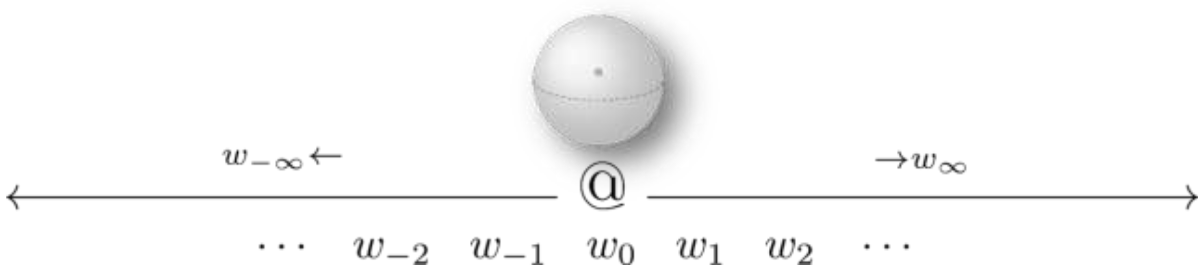
\includegraphics[width=.9\linewidth]{./images/logic-of-virtue-opposing-sequences.png}
\end{center}
\item According to the \textbf{doctrine of the mean}, there are \textbf{two extremes} (the \textbf{vices of defect} and \textbf{excess}).
\begin{center}
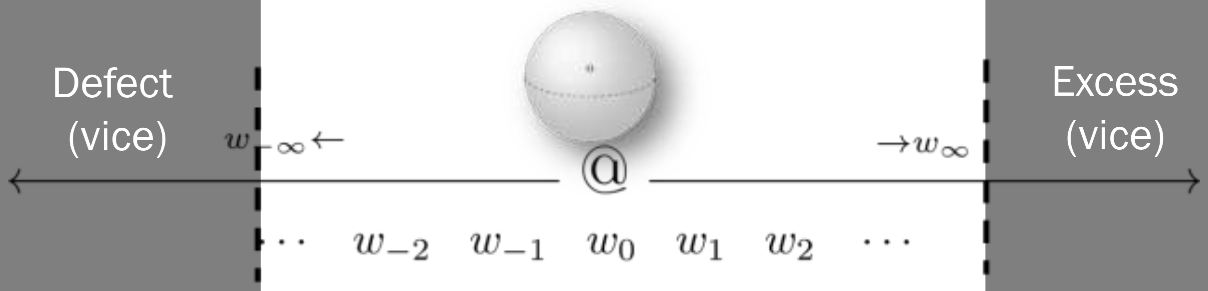
\includegraphics[width=.9\linewidth]{./images/logic-of-virtue-doctrine-of-the-mean.png}
\end{center}
\item According the \textbf{doctrine of the mean}:
\begin{center}
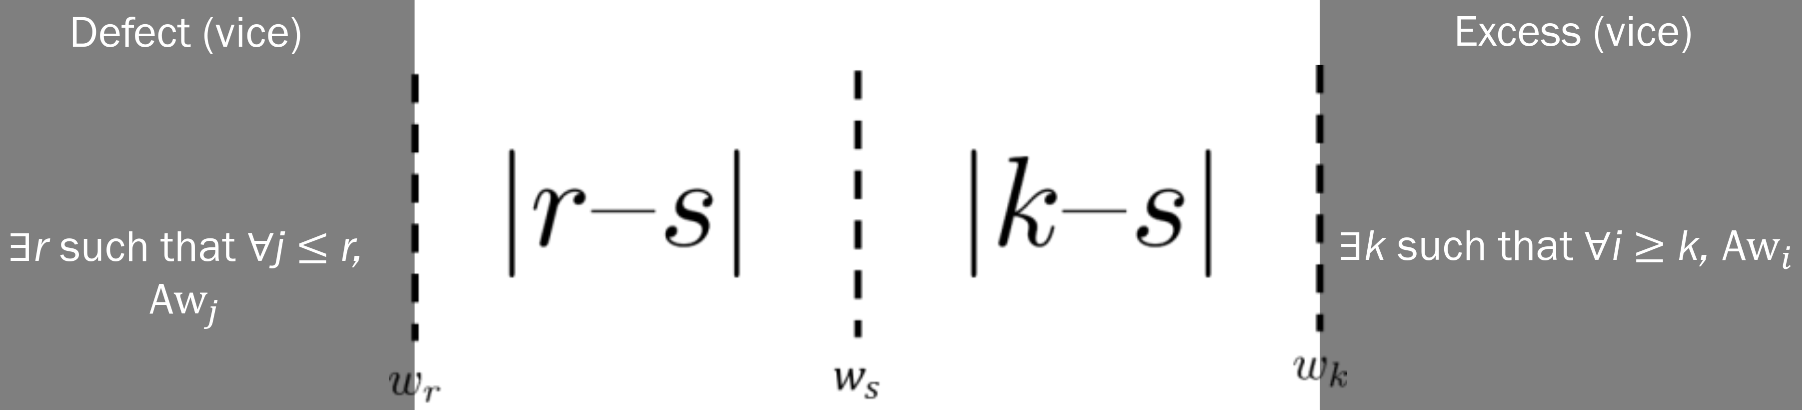
\includegraphics[width=.9\linewidth]{./images/logic-of-virtue-equation.png}
\end{center}
\begin{itemize}
\item We should choose the \textbf{life-situation} \(w_s\), where \(|r - s| = | k - s |\).
\item At \(w_s, | r - s | = | k - s |\).
\item Possible world \(w_s\) is a point that is \textbf{intermediate} between \textbf{two extremes} (the \textbf{vices of defect} and \textbf{excess}).
\end{itemize}
\end{itemize}
\subsubsection{Objections}
\label{sec:org4cd850b}
\begin{enumerate}
\item The \textbf{arithmetic mean} between 5 and 15 is \textbf{invariably} 10, whatever units we might use:
\[x = \frac{5 + 15}{2} = 10\]
By contrast, the \textbf{mean} or \textbf{intermediate point} between \textbf{two extremes} (the \textbf{vices of defect} and \textbf{excess}), as determined by an expert, will \textbf{vary from one situation to the next}.
\item While \textbf{virtuous acts} can be described in some instances in terms of an agent aiming at an act that is \textbf{intermediate between two extremes} that she rejects, certain other instances are not as susceptible to \textbf{quantitative analysis}. Aristotle agrees that it is \textbf{not an easy task} to determine the \textbf{intermediate point}.
\end{enumerate}
\subsection{Agent-based virtue ethics}
\label{sec:org2df4ec5}
According to \textbf{agent-based virtue ethics}:
\begin{itemize}
\item The \textbf{moral rightness or wrongness} of \textbf{actions} is determined in terms of the motivations and \textbf{dispositions} of the \textbf{virtuous exemplar}.
\item One problem with \textbf{eudaimonist virtue ethics} is that the \textbf{virtues} appear to be an \textbf{instrumental means} to the \textbf{end of flourishing} or \textbf{eudaimonia}.
\item However, what is good for us (the \textbf{virtues}) ought to be \textbf{foundational}.
\item In \textbf{agent-based virtue ethics}, what is good for us (the \textbf{virtues}), is \textbf{foundational}.
\item \textbf{Morality} rests on our propensity to \textbf{want to be like virtuous exemplars}.
\item However, we do not have any \textbf{criteria for goodness} in advance of identifying \textbf{virtuous exemplars}.
\end{itemize}

 \newpage
\subsubsection{Virtuous exemplars}
\label{sec:orga9c7db5}
\begin{itemize}
\item Virtuous exemplars are \textbf{foundational}.
\item \textbf{Criteria for goodness} (inferred from \textbf{virtuous exemplars}) are \textbf{derivative}.
\item It is through our identification of \textbf{virtuous exemplars} that we get our \textbf{criteria for goodness}.
\item Steps:
\begin{enumerate}
\item Identify \textbf{virtuous exemplars}.
\item Infer \textbf{criteria for goodness}.
\item Appraise \textbf{individuals actions} in terms of \textbf{virtues}.
\item Appraise \textbf{individual actions} in \textbf{deontic terms}.
\end{enumerate}
\item According to Zagzebski's version of \textbf{agent-based virtue ethics}:

\begin{center}
\begin{tabularx}{\textwidth}{|X|X|X|}
\hline
Description of action \(\phi\) in terms of virtues and vices & Description of \(\phi\) in deontic terms & Formal representation\\
\hline
\(\phi\) is a \textbf{requirement of virtue} & \(\phi\) is \textbf{obligatory} & \(O \phi\) or \(\neg P \neg \phi\)\\
\hline
\(\phi\) is neither a \textbf{requirement of virtue} nor an \textbf{expression of vice} & \(\phi\) is \textbf{permissible} & \(P \phi\)\\
\hline
\(\phi\) is \textbf{contrary to virtue} and an \textbf{expression of vice} & \(\phi\) is \textbf{impermissible} & \(\neg P \phi\) or \(O \neg \phi\)\\
\hline
\end{tabularx}
\end{center}
\end{itemize}

 \newpage
\subsection{Target-centred virtue ethics}
\label{sec:orgee4cd74}
According to \textbf{target-centred virtue ethics}:
\begin{itemize}
\item We already approve of certain \textbf{virtues}, like \textbf{confidence courage, modesty, temperance, liberality}, and so on.
\item Hence, our task is to develop a \textbf{complete account of each virtue}.
\item Since the \textbf{profiles of the virtues} are \textbf{complex}, there will be \textbf{complexity and plurality} in the requirements for virtuous action.
\item A \textbf{virtuous action} is an action that \textbf{hits the target of a virtue-profile}.
\item The \textbf{field} of each \textbf{virtue} is its \textbf{sphere of concern}:
\begin{center}
\begin{tabularx}{\textwidth}{X|X}
Field & Virtue\\
\hline
Material wealth & Liberality\\
Bodily pleasures & Temperance\\
Dangerous situations & Courage\\
\end{tabularx}
\end{center}
\item An \textbf{action} may have a \textbf{context} that involves \textbf{many different overlapping fields}.
\item \textbf{Target-centred virtue ethics} will have to move in these instances beyond the \textbf{analysis of single virtues}.
\item Hence, \textbf{target-centred virtue ethics} may have to deal with \textbf{different virtues} having \textbf{conflicting claims} on us.
\end{itemize}
\subsection{Summary}
\label{sec:org1d107a5}
\begin{enumerate}
\item Eudaimonist virtue ethics:
Virtues are traits that either \textbf{constitute} or \textbf{contribute to eudaimonia}.
\item Agent-based virtue ethics:
The \textbf{moral rightness or wrongness of actions} is determined in terms of the motivations and dispositions of the \textbf{virtuous exemplar}.
\item Target-centred virtue ethics:
Our task is to develop a \textbf{complete account of each virtue} and perform \textbf{virtuous actions}, where \textbf{virtuous actions} are actions that \textbf{hit the target} of a \textbf{virtue-profile}.
\end{enumerate}
\subsection{Objections to virtue ethics}
\label{sec:org137e54b}

\subsubsection{Egoism problem}
\label{sec:orgcbe0f26}
\begin{itemize}
\item Ethical egoism, which is defines that \(\phi\)-ing is \textbf{morally right} if and only if it \textbf{maximises the good}, where the \textbf{good} is that which \textbf{facilirates self-interest}.
\item According to \textbf{eudaimonist virtue ethics, human flourishing} is seen as an \textbf{end in itself}.
\item \textbf{Eudaimonist virtue ethics} might not sufficiently consider the extent to which our actions affect other individuals and their \textbf{life situations}.
\item Therefore, might \textbf{eudaimonist virtue ethics} not reduce to some form of \textbf{ethical egoism}?
\end{itemize}
\subsubsection{Application problem}
\label{sec:org4ce21ff}
\begin{itemize}
\item In the early days of the \textbf{neo-Aristotelian revival of virtue ethics} in response to \textbf{consequentialism} and \textbf{deontology}, virtue ethics was associated with an \textbf{anti-codifiability thesis}.
\item This \textbf{anti-codifiability thesis} entails that \textbf{virtue ethics} does not produce \textbf{codifiable action-guiding principles}.
\item However, there is a worry about \textbf{action-guidingness}.
\item \textbf{Normative theory} is nothing if not \textbf{action-guiding}.
\item However, the concern is that \textbf{virtue ethics} can only offer typically \textbf{vague advice} to act as a \textbf{virtuous person} would act in a given situation.
\end{itemize}

 \newpage
\subsubsection{Moral luck problem}
\label{sec:org357fd74}
\begin{itemize}
\item A significant aspect of what a moral agent is being assessed for \textbf{depends on factors beyond her control}.
\item The ability to cultivate the \textbf{right virtues} will be affected by a number of different \textbf{factors beyond a person's control}:
\begin{itemize}
\item Education
\item Society
\item Friends
\item Family
\item Other external goods
\end{itemize}
\item Whether or not we possess these \textbf{external goods} identified by Aristotle is a matter of \textbf{luck}.
\end{itemize}
\subsubsection{Situationist challenge}
\label{sec:org594871a}
Recent work in \textbf{situationist social psychology} shows that there are no such things as \textbf{character traits} and, thereby, no such things as \textbf{virtues} for \textbf{virtue ethics} to be about.
\subsection{Responses to objections}
\label{sec:orgb6f0c5f}

\subsubsection{Egoism problem}
\label{sec:org53f65e5}
\begin{itemize}
\item There are \textbf{self-regarding} and \textbf{other-regarding virtues}.
\item \textbf{Kindness} is an \textbf{other-regarding virtue} about how we respond to the needs of others.
\item The \textbf{good of the self} and the \textbf{good of others} are not two separate ends.
\item Both result from the exercise of \textbf{virtue}.
\item \textbf{Eudaimonist virtue ethics} unifies \textbf{what is required by morality} and \textbf{what is required by self-interest}.
\item Hence, \textbf{eudaimonist virtue ethics} does not reduce to \textbf{ethical egoism}.
\end{itemize}
\subsubsection{Application problem}
\label{sec:org1948a9c}
\begin{itemize}
\item Any \textbf{normative theory} that \textbf{fails to be action-guiding} is no good as a \textbf{normative theory}.
\item However, \textbf{agent-based virtue ethics} can be sufficiently \textbf{action-guiding}.
\item We can \textbf{observe the example of the virtuous exemplar}.
\item More generally, \textbf{virtue ethics} emphasises the role of \textbf{moral education} and \textbf{development}.
\item Knowing what to do is not a matter of \textbf{internalising a principle}.
\item Rather, knowing what to do is a lifelong process of \textbf{moral learning}.
\end{itemize}
\subsubsection{Moral luck problem}
\label{sec:orge69c7a2}
\begin{itemize}
\item The \textbf{moral luck problem} concerns the sense in which \textbf{virtue ethics} leaves us \textbf{hostage to luck}.
\item In \textbf{Aristotelian virtue ethics, friendship with other virtuous persons} is crucial.
\item However, we have no control over the \textbf{availability of the right friends}.
\item Nonetheless, \textbf{virtue ethics} embraces \textbf{moral luck}.
\item \textbf{Virtue ethics} does not try to make morality immune to matters that are beyond our control.
\item Rather, \textbf{virtue ethics} recognises the \textbf{fragility of the good life} and makes it a feature of \textbf{morality}.
\item It is only because the \textbf{good life} is \textbf{vulnerable and fragile} that it is so \textbf{precious}.
\end{itemize}

 \newpage
\subsubsection{Situationist challenge}
\label{sec:orgec285b5}
\begin{enumerate}
\item Argument from rarity
\begin{itemize}
\item \textbf{Truly virtuous people} are very \textbf{rare}.
\item Hence, \textbf{situationist literature} is entirely consistent with traditional accounts of \textbf{virtue ethics}.
\end{itemize}
\item Empirical counterchallenge
Directly \textbf{dispute the data} collected by \textbf{situationists}.
\item Immunisation thesis
\begin{itemize}
\item Armed with a better understanding of the \textbf{situationist threat}, we can use the data to \textbf{immunise or shield ourselves} from the \textbf{encroachment of morally irrelevant situationist variables} and better equip ourselves on the \textbf{virtue-ethical} front.
\end{itemize}
\item Revisionist response
\begin{itemize}
\item Accept that the \textbf{situationist data} puts serious pressure on classical accounts of \textbf{virtue ethics} and offer \textbf{revisionist or rival versions of virtue ethics} in response.
\end{itemize}
\end{enumerate}

 \newpage
\subsection{Anscombe}
\label{sec:org1078732}

\subsubsection{Theses}
\label{sec:org2078b8d}
\begin{enumerate}
\item It is not profitable for us to do \textbf{moral philosophy} until we have an adequate \textbf{philosophy of psychology}.
\item The concepts of \textbf{moral obligation and duty} ought to be \textbf{jettisoned} because they are \textbf{survivals from an earlier conception of ethics} that no longer survive.
\item The \textbf{differences between the well-known English writers on moral philosophy} from Sidgwick to the present day are of \textbf{little importance}.
\end{enumerate}
\subsubsection{Issues}
\label{sec:orga34a349}
\begin{itemize}
\item The terms "\textbf{should}" and "\textbf{ought}" have traditionally been related to \textbf{good and bad}.
\item However, the "\textbf{should}" and "\textbf{ought}" have now acquired a \textbf{special post-Aristotelian moral sense}.
\item They have been equated with the sense "\textbf{is obliged, is bound, is required to}" (by law).
\item Between Aristotle and us came \textbf{Christianity} and its \textbf{law conception of ethics}.
\end{itemize}

 \newpage
\subsubsection{Issues with consequentialism}
\label{sec:orgb783db3}
\begin{itemize}
\item Consequentialism means that it is the \textbf{consequences} that are to decide.
\item For Anscombe, \textbf{consequentialism} is a \textbf{shallow philosophy}.
\item \textbf{Consequentialism} denies any distinction between \textbf{intended and foreseen consequences}.
\item However, according to Anscombe:
\begin{itemize}
\item An agent is \textbf{responsible} for the \textbf{bad consequences} of his \textbf{bad actions}.
\item An agent gets no credit for the \textbf{good consequences} of his \textbf{bad actions}.
\item An agent is not responsible for the \textbf{bad consequences} of his \textbf{good actions}.
\end{itemize}
\item Anscombe's "Modern moral philosophy" is thought to have stimulated the development of \textbf{virtue ethics} (the \textbf{no-Aristotelian revival of virtue ethics}).
\end{itemize}
\subsubsection{Traditional interpretation of Anscombe's argument}
\label{sec:orga690823}
\begin{itemize}
\item P1: If \textbf{religiously based ethics} is \textbf{false}, then \textbf{virtue ethics} is the way \textbf{moral philosophy} ought to be developed.
\item P2: \textbf{Religiously based ethics} is false.
\item Conclusion: Hence \textbf{virtue ethics} is the way \textbf{moral philosophy} ought to be developed.
\end{itemize}

\[P1: p \rightarrow q\]
\[P2: p\]
\[C: \therefore q \ (\text{modus ponens and \textbf{valid}})\]
\subsubsection{Alternative and competing interpretation of Anscombe's argument}
\label{sec:org0400fe9}
\begin{itemize}
\item P1: If \textbf{religiously based ethics} is \textbf{false}, then \textbf{virtue ethics} is the way \textbf{moral philosophy} ought to be developed.
\item P2: It is not hte case that \textbf{virtue ethics} is the way to develop \textbf{moral philosophy}.
\item Conclusion: Therefore, it is not the case that \textbf{religiously based ethics} is false.
\end{itemize}

\[P1: p \rightarrow q\]
\[P2: \neg q\]
\[C: \therefore \neg p \ (\text{modus ponens and \textbf{valid}})\]

 \newpage
\section{Logic symbols}
\label{sec:org2a0aa89}
\begin{center}
\begin{tabular}{l|l}
Symbol & Meaning\\
\hline
\(\neg\) & Not (negation)\\
\(\vee\) & Or (disjunction)\\
\(\oplus\) & Exclusive or (exclusive disjunction)\\
\(\wedge\) & And (conjunction)\\
\(\bot\) & Always false (contradiction)\\
\(\top\) & Always true (tautology)\\
\(\forall\) & For all (universal quantification)\\
\(\exists\) & There exists (existential quantification)\\
\(\exists !\) & There exists exactly one (uniqueness quantification)\\
\(\nexists\) & There does not exist\\
\(\rightarrow\) & If \ldots{} then, implies (material conditional or implication)\\
\(\leftrightarrow\) & If and only if (material biconditional or equivalence)\\
\(\therefore\) & Therefore\\
\(\because\) & Because\\
\(\vdash\) & Proves (syntactically entails)\\
\(\nvdash\) & Does not prove (does not syntactically entail)\\
\(\vDash\) & Semantically entails\\
\(\nvDash\) & Does not semantically entail\\
\(\equiv\) & Is logically equivalent to (logical equivalence)\\
\(\Box\) & It is necessary (necessity)\\
\(\Diamond\) & It is possible (possibility)\\
\(:=\) & It is defined as (definition)\\
\(\defequal\) & It is defined as (definition)\\
\(Op\) & It is obligatory\\
\(Pp\) & It is possible\\
\(\succ\) & It is preferable\\
\(\prec\) & It is less preferable\\
\(\succeq\) & It is preferable or similar in preference\\
\(\preceq\) & It is less preferable or similar in preference\\
\(\sim\) & It is similar in preference\\
\end{tabular}
\end{center}
\end{document}
